\documentclass[twoside]{book}

% Packages required by doxygen
\usepackage{calc}
\usepackage{doxygen}
\usepackage{graphicx}
\usepackage[utf8]{inputenc}
\usepackage{makeidx}
\usepackage{multicol}
\usepackage{multirow}
\usepackage{textcomp}
\usepackage[table]{xcolor}

% Font selection
\usepackage[T1]{fontenc}
\usepackage{mathptmx}
\usepackage[scaled=.90]{helvet}
\usepackage{courier}
\usepackage{amssymb}
\usepackage{sectsty}
\renewcommand{\familydefault}{\sfdefault}
\allsectionsfont{%
  \fontseries{bc}\selectfont%
  \color{darkgray}%
}
\renewcommand{\DoxyLabelFont}{%
  \fontseries{bc}\selectfont%
  \color{darkgray}%
}

% Page & text layout
\usepackage{geometry}
\geometry{%
  a4paper,%
  top=2.5cm,%
  bottom=2.5cm,%
  left=2.5cm,%
  right=2.5cm%
}
\tolerance=750
\hfuzz=15pt
\hbadness=750
\setlength{\emergencystretch}{15pt}
\setlength{\parindent}{0cm}
\setlength{\parskip}{0.2cm}
\makeatletter
\renewcommand{\paragraph}{%
  \@startsection{paragraph}{4}{0ex}{-1.0ex}{1.0ex}{%
    \normalfont\normalsize\bfseries\SS@parafont%
  }%
}
\renewcommand{\subparagraph}{%
  \@startsection{subparagraph}{5}{0ex}{-1.0ex}{1.0ex}{%
    \normalfont\normalsize\bfseries\SS@subparafont%
  }%
}
\makeatother

% Headers & footers
\usepackage{fancyhdr}
\pagestyle{fancyplain}
\fancyhead[LE]{\fancyplain{}{\bfseries\thepage}}
\fancyhead[CE]{\fancyplain{}{}}
\fancyhead[RE]{\fancyplain{}{\bfseries\leftmark}}
\fancyhead[LO]{\fancyplain{}{\bfseries\rightmark}}
\fancyhead[CO]{\fancyplain{}{}}
\fancyhead[RO]{\fancyplain{}{\bfseries\thepage}}
\fancyfoot[LE]{\fancyplain{}{}}
\fancyfoot[CE]{\fancyplain{}{}}
\fancyfoot[RE]{\fancyplain{}{\bfseries\scriptsize Generated on Thu Jul 2 2015 04\-:02\-:29 for Open Sencillo by Doxygen }}
\fancyfoot[LO]{\fancyplain{}{\bfseries\scriptsize Generated on Thu Jul 2 2015 04\-:02\-:29 for Open Sencillo by Doxygen }}
\fancyfoot[CO]{\fancyplain{}{}}
\fancyfoot[RO]{\fancyplain{}{}}
\renewcommand{\footrulewidth}{0.4pt}
\renewcommand{\chaptermark}[1]{%
  \markboth{#1}{}%
}
\renewcommand{\sectionmark}[1]{%
  \markright{\thesection\ #1}%
}

% Indices & bibliography
\usepackage{natbib}
\usepackage[titles]{tocloft}
\setcounter{tocdepth}{3}
\setcounter{secnumdepth}{5}
\makeindex

% Hyperlinks (required, but should be loaded last)
\usepackage{ifpdf}
\ifpdf
  \usepackage[pdftex,pagebackref=true]{hyperref}
\else
  \usepackage[ps2pdf,pagebackref=true]{hyperref}
\fi
\hypersetup{%
  colorlinks=true,%
  linkcolor=blue,%
  citecolor=blue,%
  unicode%
}

% Custom commands
\newcommand{\clearemptydoublepage}{%
  \newpage{\pagestyle{empty}\cleardoublepage}%
}


%===== C O N T E N T S =====

\begin{document}

% Titlepage & ToC
\hypersetup{pageanchor=false}
\pagenumbering{roman}
\begin{titlepage}
\vspace*{7cm}
\begin{center}%
{\Large Open Sencillo \\[1ex]\large 2015.\-107 }\\
\vspace*{1cm}
{\large Generated by Doxygen 1.8.6}\\
\vspace*{0.5cm}
{\small Thu Jul 2 2015 04:02:29}\\
\end{center}
\end{titlepage}
\clearemptydoublepage
\tableofcontents
\clearemptydoublepage
\pagenumbering{arabic}
\hypersetup{pageanchor=true}

%--- Begin generated contents ---
\chapter{P\-A\-G\-E}
\label{string}
\hypertarget{string}{}
Get page by P\-A\-G\-E 
\chapter{\#Open\-Sencillo}
\label{md__home_peter_git__open_sencillo__r_e_a_d_m_e}
\hypertarget{md__home_peter_git__open_sencillo__r_e_a_d_m_e}{}
\subsection*{Open\-Sencillo P\-H\-P framework}

\begin{quotation}
Help with programming Open\-Sencillo P\-H\-P Framework. {\itshape We are looking for you!}

\end{quotation}


\subsubsection*{About Stable version}

\begin{quotation}

\begin{DoxyItemize}
\item Name\-: Open\-Sencillo;
\item Licence\-: \href{http://www.gnu.org/licenses/gpl-3.0.html}{\tt G\-N\-U/\-G\-P\-L};
\item Type\-: Framework;
\item Category\-: Open\-Source;
\item Language\-: P\-H\-P 5.\-3+, J\-Q\-U\-E\-R\-Y, H\-T\-M\-L5
\item Year\-: 2015;
\item Build\-: 107;
\item Rev\-: 2015.\-107;
\item By\-: \href{http://phorvath.com}{\tt Bc. Peter Horváth};
\item Homepage\-: \href{http://opensencillo.com}{\tt Open Sencillo};
\item Features\-: File management, File Convertors, Database management, S\-E\-O, Session \& Cookies management, Hash subsystem, Translates J\-S\-O\-N file, Unit Testing, Htaccess generator, Simple image tool ...
\end{DoxyItemize}

\end{quotation}


\section*{\#\#\-How to Install }

Check\-: \href{http://www.opensencillo.com/installation/}{\tt http\-://www.\-opensencillo.\-com/installation/}

\section*{\#\#\-Examples }

Check\-: \href{http://www.opensencillo.com/sencillo-php-examples/}{\tt http\-://www.\-opensencillo.\-com/sencillo-\/php-\/examples/}

\subsection*{Module types}

\subsubsection*{Name structure}

In version $>$= 2015.\-003 \begin{quotation}
\mbox{[}type\mbox{]}\-\_\-\mbox{[}module-\/name\mbox{]}.php

\end{quotation}


\paragraph*{Types\-:}


\begin{DoxyItemize}
\item module
\item info
\item install
\item update
\end{DoxyItemize}

\subsection*{Library files}

It is special modules contains system´s classes.

\section*{\#\#\-Changes log }

\subsubsection*{O\-N B\-U\-I\-L\-D 2015.\-108}

\subsubsection*{2015.\-107}

\subsubsection*{2015.\-106}

\subsubsection*{2015.\-105}

\subsubsection*{2015.\-005}


\begin{DoxyEnumerate}
\item New welcome page
\item Fix \#17 database foreign key problem
\item New structgen class for generating menu or galleries
\item Update manager tool \#3 -\/ no gui
\item Paylock subsystem -\/ update
\item Add O\-G tags
\item Add Snippet meta tags
\item Fix Snippet bug
\item Fix first start database login problems
\item Add menu generator
\item Fix foreigns keys in core\-\_\-sql
\item Create config class for database layout
\item Add support config class in core\-\_\-sql
\item Add \hyperlink{structure_8generator_8structgen_8php_source}{structure.\-generator.\-structgen.\-php} for generate universal structures
\item Add \hyperlink{google_8analytics_8goas_8php_source}{google.\-analytics.\-goas.\-php} library for support Google Universal Analytics
\item Add \hyperlink{classboot_up}{boot\-Up} class for in class loading sencillo
\end{DoxyEnumerate}

\subsubsection*{2015.\-004}


\begin{DoxyEnumerate}
\item Fix \#9 add io\-\_\-validator in to Sencillo C\-O\-R\-E
\item Add Mastery product key validator
\item Add Mastery system key lock
\item Add float parser
\item Add object interface for core
\item Add welcome page (in yourcode.\-php)
\item Fix installation bug
\end{DoxyEnumerate}

\subsubsection*{2015.\-003}


\begin{DoxyEnumerate}
\item New structure for module\-: \mbox{[}type\mbox{]}\-\_\-\mbox{[}module-\/name\mbox{]}.php
\item Fix \#5 lib\-\_\-identificator is used for read modules
\item Add bootstrap for C\-S\-S3
\item Add bootstrap pretty installer
\item Add relocation installer if sencillo not installed
\item Add new My\-S\-Q\-L Interface
\item Cache defaults O\-F\-F
\item Gzip cache if allow
\item Add mysql full outer join
\item Add mysql left join
\item Add mysql right join
\item Add mysql inner join
\item Add action aliases
\item Add mysqli update
\item Add mysqli insert
\item Convert to G\-P\-L3
\item Add security hash
\item Add I\-N\-S\-E\-R\-T to S\-Q\-L installer
\item Add \hyperlink{namespace_simple_image}{Simple\-Image} library
\item Close issue \#2 -\/ add new htaccess generator (library only; test need)
\end{DoxyEnumerate}

\subsubsection*{2015.\-002}


\begin{DoxyEnumerate}
\item Add mysql core function\-: unique\-Key
\item Add mysql core function\-: prepare\-Table
\item Add testing tool in to \hyperlink{test_8tool_8framework_8php_source}{test.\-tool.\-framework.\-php}
\item Add testing tool function output to browser console\-: print\-\_\-ut,print\-\_\-test
\item Removed nonobject files
\item Comment old cookie system and old session system (as depecrated)
\item Full comment main config (as depecrated)
\item Fix \#1 Installer problem\-: Problem 1,3 solved
\end{DoxyEnumerate}

\subsubsection*{2015.\-001}


\begin{DoxyEnumerate}
\item Add default login template
\item Add default registration template
\item Add default account template
\item Add installer main screen template
\item Add logman default login function
\end{DoxyEnumerate}

\subsubsection*{2014.\-012}


\begin{DoxyEnumerate}
\item Add library support system lib\-\_\-identificator
\item Add exception for load lib\-\_\-identification
\item Add information subsystem
\item Repair mod\-\_\-indentificator path
\item Add back support for old Sencillos
\item Add lib\-\_\-identificator to bootstrap
\item Add library for delete files named file.\-delete.\-fdel.\-php
\item Fix core bugs in open\-Table
\item Fix logman support version 2014.\-012
\item Root folder \char`\"{}framework\char`\"{} set as variable subfolder
\item Add check session to logman
\item Add login by logman via hash sha512
\item Fix translate tool (translate file not exist)
\item Add create translate
\item Add cache allow / disallow
\end{DoxyEnumerate}

\subsubsection*{2014.\-011}


\begin{DoxyEnumerate}
\item Repair install path
\item Add P\-D\-F2\-J\-P\-G support
\item Add prebuild path to jquery
\item Add translate library
\end{DoxyEnumerate}

\subsubsection*{2014.\-010}

\subsubsection*{2014.\-009}

\subsubsection*{2014.\-008}


\begin{DoxyEnumerate}
\item Add back compatible mode
\item Upgrade installer from version 2014.\-005 to 2014.\-008
\item Upgrade broken path in installer
\item Upgrade broken path in core
\item Add new path in core chmod
\item Delete boxid from default install mode
\item Upgrade to nodatabase module installer mod\-\_\-identificator.\-php
\item Add database select
\item Add G\-N\-U G\-P\-L terms
\end{DoxyEnumerate}

\subsubsection*{2014.\-007}


\begin{DoxyEnumerate}
\item Rename folders cms\-\_\-$\ast$ to fw\-\_\-$\ast$
\item Merged developer version to version 2014.\-007
\item Upgrade mod\-\_\-identificator.\-php from version 2014.\-002 to 2014.\-007
\item Add default libraries
\item Rename root folder \char`\"{}cms\char`\"{} to root folder \char`\"{}framework\char`\"{}
\end{DoxyEnumerate}

\section*{\#\#\-Older }

\subsubsection*{O\-B\-S\-O\-L\-E\-T\-E 2014.\-006 A\-N\-D O\-L\-D\-E\-R}


\begin{DoxyEnumerate}
\item Minimal support for modules 2014.\-007 and up
\item Not support library
\item Old layout subsystem
\item Instalation problems in 2014.\-005 and older
\item Security subsystem problem 
\end{DoxyEnumerate}
\chapter{Namespace Index}
\section{Namespace List}
Here is a list of all documented namespaces with brief descriptions\-:\begin{DoxyCompactList}
\item\contentsline{section}{\hyperlink{namespace_simple_image}{Simple\-Image} }{\pageref{namespace_simple_image}}{}
\end{DoxyCompactList}

\chapter{Hierarchical Index}
\section{Class Hierarchy}
This inheritance list is sorted roughly, but not completely, alphabetically\-:\begin{DoxyCompactList}
\item \contentsline{section}{analytics}{\pageref{classanalytics}}{}
\item \contentsline{section}{boot\-Up}{\pageref{classboot_up}}{}
\item \contentsline{section}{clist}{\pageref{classclist}}{}
\item \contentsline{section}{core\-Interface}{\pageref{interfacecore_interface}}{}
\begin{DoxyCompactList}
\item \contentsline{section}{core\-Sencillo}{\pageref{classcore_sencillo}}{}
\end{DoxyCompactList}
\item \contentsline{section}{fdel}{\pageref{classfdel}}{}
\item \contentsline{section}{files\-List}{\pageref{classfiles_list}}{}
\item \contentsline{section}{file\-System}{\pageref{classfile_system}}{}
\begin{DoxyCompactList}
\item \contentsline{section}{file}{\pageref{classfile}}{}
\item \contentsline{section}{translate}{\pageref{classtranslate}}{}
\end{DoxyCompactList}
\item \contentsline{section}{form\-Creator}{\pageref{classform_creator}}{}
\item \contentsline{section}{get\-Cookies}{\pageref{classget_cookies}}{}
\item \contentsline{section}{header\-Seo}{\pageref{classheader_seo}}{}
\item \contentsline{section}{htgen}{\pageref{classhtgen}}{}
\item \contentsline{section}{input\-Rewrite}{\pageref{classinput_rewrite}}{}
\item \contentsline{section}{library}{\pageref{classlibrary}}{}
\item \contentsline{section}{log}{\pageref{classlog}}{}
\begin{DoxyCompactList}
\item \contentsline{section}{unit\-Test}{\pageref{classunit_test}}{}
\end{DoxyCompactList}
\item \contentsline{section}{menu\-Gen}{\pageref{classmenu_gen}}{}
\item \contentsline{section}{mysql}{\pageref{classmysql}}{}
\begin{DoxyCompactList}
\item \contentsline{section}{mysql\-Edit}{\pageref{classmysql_edit}}{}
\begin{DoxyCompactList}
\item \contentsline{section}{log\-Man}{\pageref{classlog_man}}{}
\item \contentsline{section}{mysql\-Interface}{\pageref{classmysql_interface}}{}
\end{DoxyCompactList}
\end{DoxyCompactList}
\item \contentsline{section}{P\-D\-Fto\-J\-P\-G}{\pageref{class_p_d_fto_j_p_g}}{}
\item \contentsline{section}{session\-Manager}{\pageref{classsession_manager}}{}
\begin{DoxyCompactList}
\item \contentsline{section}{login\-Manager}{\pageref{classlogin_manager}}{}
\end{DoxyCompactList}
\item \contentsline{section}{Simple\-Image}{\pageref{classabeautifulsite_1_1_simple_image}}{}
\item \contentsline{section}{structgen}{\pageref{classstructgen}}{}
\begin{DoxyCompactList}
\item \contentsline{section}{default\-Structures}{\pageref{classdefault_structures}}{}
\end{DoxyCompactList}
\item \contentsline{section}{upload}{\pageref{classupload}}{}
\item \contentsline{section}{url}{\pageref{classurl}}{}
\item \contentsline{section}{User\-Agent\-Parser}{\pageref{class_user_agent_parser}}{}
\end{DoxyCompactList}

\chapter{Data Structure Index}
\section{Data Structures}
Here are the data structures with brief descriptions\-:\begin{DoxyCompactList}
\item\contentsline{section}{\hyperlink{classanalytics}{analytics} }{\pageref{classanalytics}}{}
\item\contentsline{section}{\hyperlink{classboot_up}{boot\-Up} }{\pageref{classboot_up}}{}
\item\contentsline{section}{\hyperlink{classclist}{clist} }{\pageref{classclist}}{}
\item\contentsline{section}{\hyperlink{interfacecore_interface}{core\-Interface} }{\pageref{interfacecore_interface}}{}
\item\contentsline{section}{\hyperlink{classcore_sencillo}{core\-Sencillo} }{\pageref{classcore_sencillo}}{}
\item\contentsline{section}{\hyperlink{classdefault_structures}{default\-Structures} }{\pageref{classdefault_structures}}{}
\item\contentsline{section}{\hyperlink{classfdel}{fdel} }{\pageref{classfdel}}{}
\item\contentsline{section}{\hyperlink{classfile}{file} }{\pageref{classfile}}{}
\item\contentsline{section}{\hyperlink{classfiles_list}{files\-List} }{\pageref{classfiles_list}}{}
\item\contentsline{section}{\hyperlink{classfile_system}{file\-System} }{\pageref{classfile_system}}{}
\item\contentsline{section}{\hyperlink{classform_creator}{form\-Creator} }{\pageref{classform_creator}}{}
\item\contentsline{section}{\hyperlink{classget_cookies}{get\-Cookies} }{\pageref{classget_cookies}}{}
\item\contentsline{section}{\hyperlink{classheader_seo}{header\-Seo} }{\pageref{classheader_seo}}{}
\item\contentsline{section}{\hyperlink{classhtgen}{htgen} }{\pageref{classhtgen}}{}
\item\contentsline{section}{\hyperlink{classinput_rewrite}{input\-Rewrite} }{\pageref{classinput_rewrite}}{}
\item\contentsline{section}{\hyperlink{classlibrary}{library} }{\pageref{classlibrary}}{}
\item\contentsline{section}{\hyperlink{classlog}{log} }{\pageref{classlog}}{}
\item\contentsline{section}{\hyperlink{classlogin_manager}{login\-Manager} }{\pageref{classlogin_manager}}{}
\item\contentsline{section}{\hyperlink{classlog_man}{log\-Man} }{\pageref{classlog_man}}{}
\item\contentsline{section}{\hyperlink{classmenu_gen}{menu\-Gen} }{\pageref{classmenu_gen}}{}
\item\contentsline{section}{\hyperlink{classmysql}{mysql} }{\pageref{classmysql}}{}
\item\contentsline{section}{\hyperlink{classmysql_edit}{mysql\-Edit} }{\pageref{classmysql_edit}}{}
\item\contentsline{section}{\hyperlink{classmysql_interface}{mysql\-Interface} }{\pageref{classmysql_interface}}{}
\item\contentsline{section}{\hyperlink{class_p_d_fto_j_p_g}{P\-D\-Fto\-J\-P\-G} }{\pageref{class_p_d_fto_j_p_g}}{}
\item\contentsline{section}{\hyperlink{classsession_manager}{session\-Manager} }{\pageref{classsession_manager}}{}
\item\contentsline{section}{\hyperlink{classabeautifulsite_1_1_simple_image}{Simple\-Image} }{\pageref{classabeautifulsite_1_1_simple_image}}{}
\item\contentsline{section}{\hyperlink{classstructgen}{structgen} }{\pageref{classstructgen}}{}
\item\contentsline{section}{\hyperlink{classtranslate}{translate} }{\pageref{classtranslate}}{}
\item\contentsline{section}{\hyperlink{classunit_test}{unit\-Test} }{\pageref{classunit_test}}{}
\item\contentsline{section}{\hyperlink{classupload}{upload} }{\pageref{classupload}}{}
\item\contentsline{section}{\hyperlink{classurl}{url} }{\pageref{classurl}}{}
\item\contentsline{section}{\hyperlink{class_user_agent_parser}{User\-Agent\-Parser} }{\pageref{class_user_agent_parser}}{}
\end{DoxyCompactList}

\chapter{Namespace Documentation}
\hypertarget{namespace_simple_image}{\section{Simple\-Image Namespace Reference}
\label{namespace_simple_image}\index{Simple\-Image@{Simple\-Image}}
}


\subsection{Detailed Description}
class \begin{DoxyVersion}{Version}
2.\-5.\-3 
\end{DoxyVersion}
\begin{DoxyAuthor}{Author}
Cory La\-Viska for A Beautiful Site, L\-L\-C. (\href{http://www.abeautifulsite.net/}{\tt http\-://www.\-abeautifulsite.\-net/}) 

Nazar Mokrynskyi \href{mailto:nazar@mokrynskyi.com}{\tt nazar@mokrynskyi.\-com} -\/ merging of forks, namespace support, Php\-Doc editing, adaptive\-\_\-resize() method, other fixes  This software is licensed under the M\-I\-T license\-: \href{http://opensource.org/licenses/MIT}{\tt http\-://opensource.\-org/licenses/\-M\-I\-T} 
\end{DoxyAuthor}
\begin{DoxyCopyright}{Copyright}
A Beautiful Site, L\-L\-C.
\end{DoxyCopyright}
Class \hyperlink{namespace_simple_image}{Simple\-Image} This class makes image manipulation in P\-H\-P as simple as possible. 
\chapter{Data Structure Documentation}
\hypertarget{classanalytics}{\section{analytics Class Reference}
\label{classanalytics}\index{analytics@{analytics}}
}
\subsection*{Public Member Functions}
\begin{DoxyCompactItemize}
\item 
\hyperlink{classanalytics_ae87717e51772c9cbc91f0e87afc7d00e}{set} (\$pref, \$value, \$param)
\item 
\hyperlink{classanalytics_a9be85fe710feedcbe1424b64b9dade9e}{gadefault} (\$id)
\item 
\hyperlink{classanalytics_a435e7d7525d4bcd0ed5e34a469f3adf6}{create} ()
\end{DoxyCompactItemize}
\subsection*{Protected Attributes}
\begin{DoxyCompactItemize}
\item 
\hypertarget{classanalytics_a63bb4c41bc532baacf6a4976cfaa0feb}{{\bfseries \$arr}}\label{classanalytics_a63bb4c41bc532baacf6a4976cfaa0feb}

\end{DoxyCompactItemize}


\subsection{Detailed Description}


Definition at line 11 of file google.\-analytics.\-goas.\-php.



\subsection{Member Function Documentation}
\hypertarget{classanalytics_a435e7d7525d4bcd0ed5e34a469f3adf6}{\index{analytics@{analytics}!create@{create}}
\index{create@{create}!analytics@{analytics}}
\subsubsection[{create}]{\setlength{\rightskip}{0pt plus 5cm}create (
\begin{DoxyParamCaption}
{}
\end{DoxyParamCaption}
)}}\label{classanalytics_a435e7d7525d4bcd0ed5e34a469f3adf6}
Create Google Analytics Code 

Definition at line 55 of file google.\-analytics.\-goas.\-php.

\hypertarget{classanalytics_a9be85fe710feedcbe1424b64b9dade9e}{\index{analytics@{analytics}!gadefault@{gadefault}}
\index{gadefault@{gadefault}!analytics@{analytics}}
\subsubsection[{gadefault}]{\setlength{\rightskip}{0pt plus 5cm}gadefault (
\begin{DoxyParamCaption}
\item[{}]{\$id}
\end{DoxyParamCaption}
)}}\label{classanalytics_a9be85fe710feedcbe1424b64b9dade9e}
Set G\-A to default basic options 
\begin{DoxyParams}{Parameters}
{\em \$id} & string (U\-A-\/\-X\-X\-X\-X-\/\-Y) \\
\hline
\end{DoxyParams}


Definition at line 46 of file google.\-analytics.\-goas.\-php.

\hypertarget{classanalytics_ae87717e51772c9cbc91f0e87afc7d00e}{\index{analytics@{analytics}!set@{set}}
\index{set@{set}!analytics@{analytics}}
\subsubsection[{set}]{\setlength{\rightskip}{0pt plus 5cm}set (
\begin{DoxyParamCaption}
\item[{}]{\$pref, }
\item[{}]{\$value, }
\item[{}]{\$param}
\end{DoxyParamCaption}
)}}\label{classanalytics_ae87717e51772c9cbc91f0e87afc7d00e}
Add custom universal analytics 
\begin{DoxyParams}{Parameters}
{\em \$pref} & string (create$\vert$send$\vert$require) \\
\hline
{\em \$value} & string (U\-A-\/\-X\-X\-X\-X-\/\-Y$\vert$pageview$\vert$...) \\
\hline
{\em \$param} & string (auto$\vert$...) \\
\hline
\end{DoxyParams}


Definition at line 30 of file google.\-analytics.\-goas.\-php.



The documentation for this class was generated from the following file\-:\begin{DoxyCompactItemize}
\item 
/home/peter/git/\-Open\-Sencillo/fw\-\_\-libraries/google.\-analytics.\-goas.\-php\end{DoxyCompactItemize}

\hypertarget{classboot_up}{\section{boot\-Up Class Reference}
\label{classboot_up}\index{boot\-Up@{boot\-Up}}
}
\subsection*{Public Member Functions}
\begin{DoxyCompactItemize}
\item 
\hypertarget{classboot_up_ab7f16f959f74a634ca046420bd58c74b}{{\bfseries \-\_\-\-\_\-construct} (\$sum=false)}\label{classboot_up_ab7f16f959f74a634ca046420bd58c74b}

\end{DoxyCompactItemize}
\subsection*{Data Fields}
\begin{DoxyCompactItemize}
\item 
\hypertarget{classboot_up_a4ca9ecfa22bed04c85e24326a037cfd0}{{\bfseries \$core\-Sencillo}}\label{classboot_up_a4ca9ecfa22bed04c85e24326a037cfd0}

\item 
\hypertarget{classboot_up_a7281af4d471cc5f2e00d975905db660e}{{\bfseries \$header\-Seo}}\label{classboot_up_a7281af4d471cc5f2e00d975905db660e}

\item 
\hypertarget{classboot_up_a2b06fe777e2d4bac3ef970c8a984edaa}{{\bfseries \$file\-System}}\label{classboot_up_a2b06fe777e2d4bac3ef970c8a984edaa}

\end{DoxyCompactItemize}


\subsection{Detailed Description}


Definition at line 555 of file core\-\_\-functions.\-php.



The documentation for this class was generated from the following file\-:\begin{DoxyCompactItemize}
\item 
/home/peter/git/\-Open\-Sencillo/fw\-\_\-core/core\-\_\-functions.\-php\end{DoxyCompactItemize}

\hypertarget{classclist}{\section{clist Class Reference}
\label{classclist}\index{clist@{clist}}
}
\subsection*{Public Member Functions}
\begin{DoxyCompactItemize}
\item 
\hyperlink{classclist_ae34ce6f4a6d015926997a6a1b2a84e75}{get\-Country} (\$key)
\item 
\hyperlink{classclist_aa10fd0ee87130ab7868db782f789a57d}{country\-List} ()
\end{DoxyCompactItemize}
\subsection*{Protected Attributes}
\begin{DoxyCompactItemize}
\item 
\hypertarget{classclist_a6efc15b5a2314dd4b5aaa556a375c6d6}{{\bfseries \$data}}\label{classclist_a6efc15b5a2314dd4b5aaa556a375c6d6}

\end{DoxyCompactItemize}


\subsection{Detailed Description}


Definition at line 2 of file country.\-list.\-clist.\-php.



\subsection{Member Function Documentation}
\hypertarget{classclist_aa10fd0ee87130ab7868db782f789a57d}{\index{clist@{clist}!country\-List@{country\-List}}
\index{country\-List@{country\-List}!clist@{clist}}
\subsubsection[{country\-List}]{\setlength{\rightskip}{0pt plus 5cm}country\-List (
\begin{DoxyParamCaption}
{}
\end{DoxyParamCaption}
)}}\label{classclist_aa10fd0ee87130ab7868db782f789a57d}
Return country list \begin{DoxyReturn}{Returns}
array country list 
\end{DoxyReturn}


Definition at line 297 of file country.\-list.\-clist.\-php.

\hypertarget{classclist_ae34ce6f4a6d015926997a6a1b2a84e75}{\index{clist@{clist}!get\-Country@{get\-Country}}
\index{get\-Country@{get\-Country}!clist@{clist}}
\subsubsection[{get\-Country}]{\setlength{\rightskip}{0pt plus 5cm}get\-Country (
\begin{DoxyParamCaption}
\item[{}]{\$key}
\end{DoxyParamCaption}
)}}\label{classclist_ae34ce6f4a6d015926997a6a1b2a84e75}
Get country name by I\-D 
\begin{DoxyParams}[1]{Parameters}
string & {\em \$key} & \\
\hline
\end{DoxyParams}
\begin{DoxyReturn}{Returns}
string name by \$key 
\end{DoxyReturn}


Definition at line 281 of file country.\-list.\-clist.\-php.



The documentation for this class was generated from the following file\-:\begin{DoxyCompactItemize}
\item 
/home/peter/git/\-Open\-Sencillo/fw\-\_\-libraries/country.\-list.\-clist.\-php\end{DoxyCompactItemize}

\hypertarget{interfacecore_interface}{\section{core\-Interface Interface Reference}
\label{interfacecore_interface}\index{core\-Interface@{core\-Interface}}
}
Inheritance diagram for core\-Interface\-:\begin{figure}[H]
\begin{center}
\leavevmode
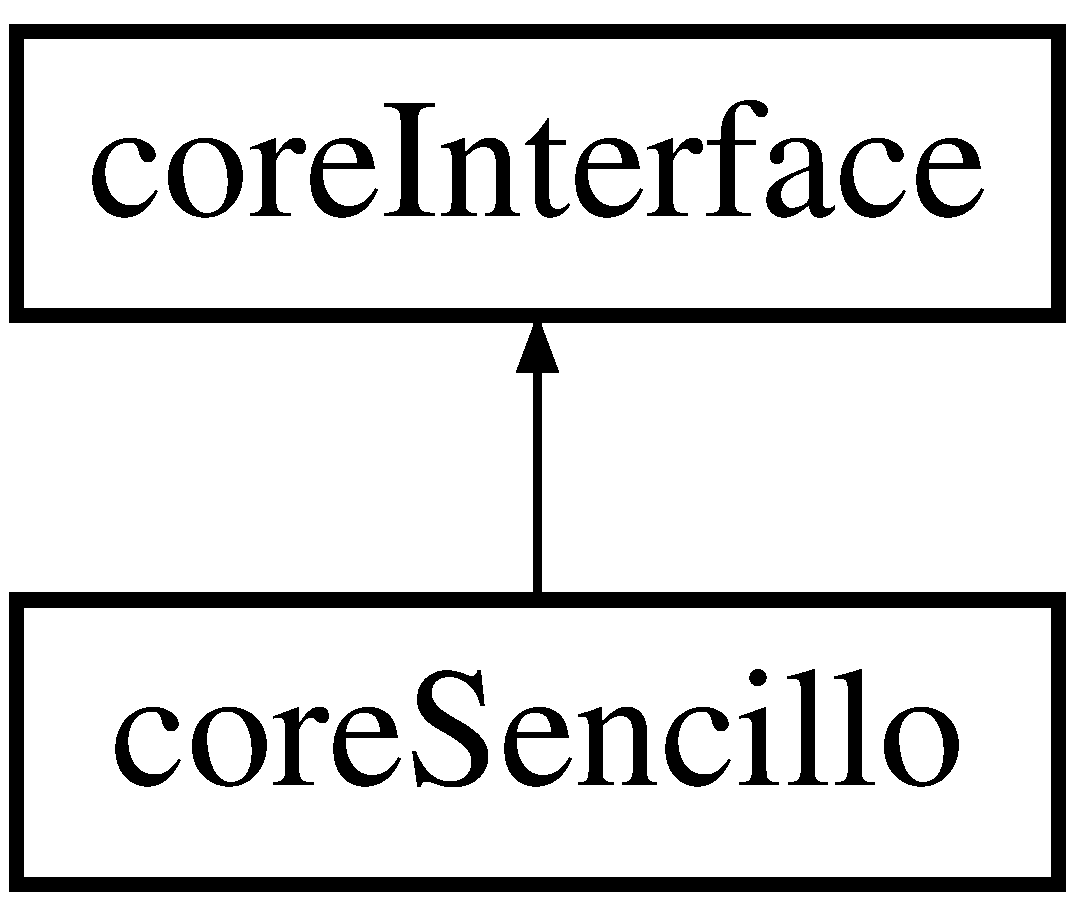
\includegraphics[height=2.000000cm]{interfacecore_interface}
\end{center}
\end{figure}
\subsection*{Public Member Functions}
\begin{DoxyCompactItemize}
\item 
\hypertarget{interfacecore_interface_a7664184e15f00825b54ecf378cd4174f}{{\bfseries version\-\_\-info} ()}\label{interfacecore_interface_a7664184e15f00825b54ecf378cd4174f}

\item 
\hypertarget{interfacecore_interface_aa88fe4a9dd8795c065f2620947d450db}{{\bfseries product} ()}\label{interfacecore_interface_aa88fe4a9dd8795c065f2620947d450db}

\item 
\hypertarget{interfacecore_interface_af4cf8181fcda31ba0ce060121795c5dc}{{\bfseries pay\-Lock} ()}\label{interfacecore_interface_af4cf8181fcda31ba0ce060121795c5dc}

\end{DoxyCompactItemize}


\subsection{Detailed Description}
Core static interface 

Definition at line 5 of file core\-\_\-interface.\-php.



The documentation for this interface was generated from the following file\-:\begin{DoxyCompactItemize}
\item 
/home/peter/git/\-Open\-Sencillo/fw\-\_\-core/core\-\_\-interface.\-php\end{DoxyCompactItemize}

\hypertarget{classcore_sencillo}{\section{core\-Sencillo Class Reference}
\label{classcore_sencillo}\index{core\-Sencillo@{core\-Sencillo}}
}
Inheritance diagram for core\-Sencillo\-:\begin{figure}[H]
\begin{center}
\leavevmode
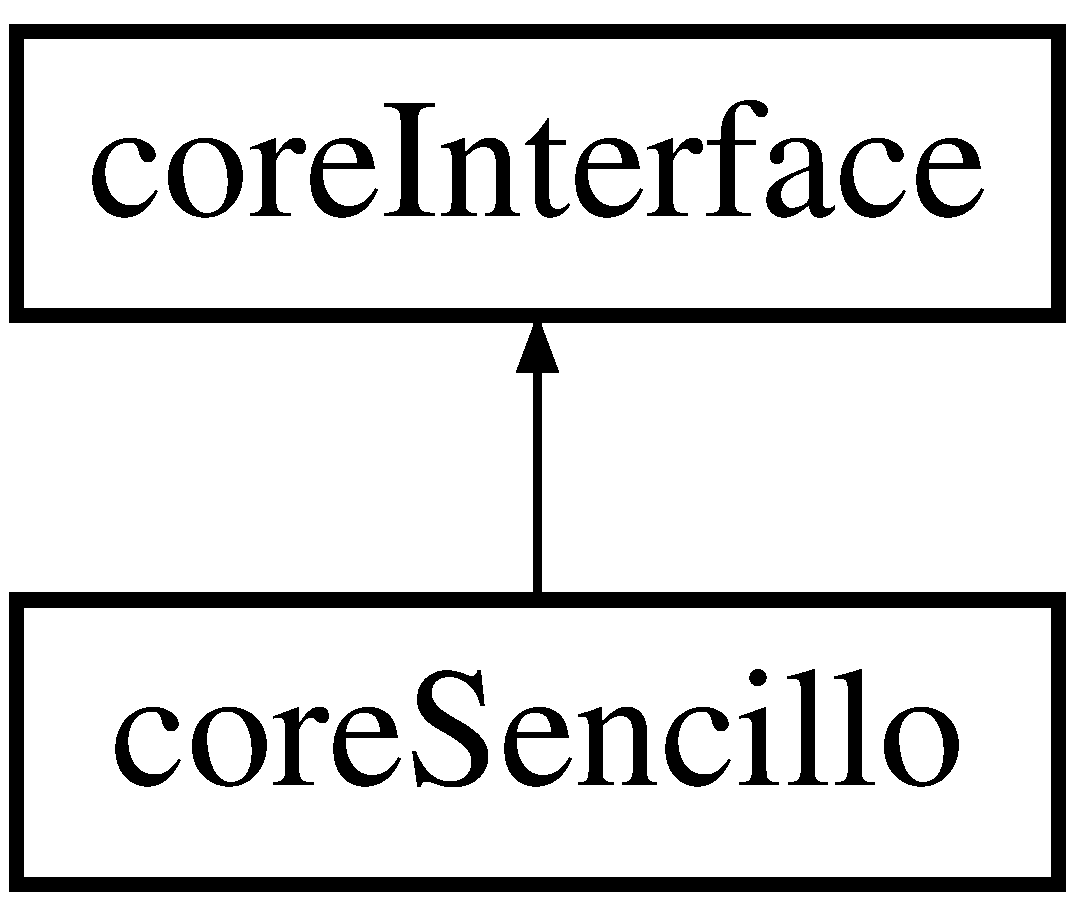
\includegraphics[height=2.000000cm]{classcore_sencillo}
\end{center}
\end{figure}
\subsection*{Public Member Functions}
\begin{DoxyCompactItemize}
\item 
\hyperlink{classcore_sencillo_a4fd5742704d00ae15f527894bcd8cfb9}{\-\_\-\-\_\-construct} (\$sum=null)
\item 
\hypertarget{classcore_sencillo_a7664184e15f00825b54ecf378cd4174f}{{\bfseries version\-\_\-info} ()}\label{classcore_sencillo_a7664184e15f00825b54ecf378cd4174f}

\item 
\hypertarget{classcore_sencillo_a2c7c8f0c4ae866f7c7f9956739d39696}{{\bfseries authorized} (\$domains)}\label{classcore_sencillo_a2c7c8f0c4ae866f7c7f9956739d39696}

\item 
\hyperlink{classcore_sencillo_a62e12d2cf1dbc3c01d867a76d26adf65}{product} (\$path=false)
\item 
\hyperlink{classcore_sencillo_af4cf8181fcda31ba0ce060121795c5dc}{pay\-Lock} ()
\item 
\hypertarget{classcore_sencillo_af357eccac1f8e7e9df4c1491a92bd0f1}{{\bfseries upgrade} (\$source=null)}\label{classcore_sencillo_af357eccac1f8e7e9df4c1491a92bd0f1}

\end{DoxyCompactItemize}
\subsection*{Data Fields}
\begin{DoxyCompactItemize}
\item 
\hypertarget{classcore_sencillo_ae19722790c6683980bbf0af8572f26ab}{{\bfseries \$info}}\label{classcore_sencillo_ae19722790c6683980bbf0af8572f26ab}

\item 
\hypertarget{classcore_sencillo_abb35c8495a232b510389fa6d7b15d38a}{{\bfseries \$request}}\label{classcore_sencillo_abb35c8495a232b510389fa6d7b15d38a}

\item 
\hypertarget{classcore_sencillo_afc86bce95fea4d2f4bd9e481e66754ff}{{\bfseries \$original\-\_\-request}}\label{classcore_sencillo_afc86bce95fea4d2f4bd9e481e66754ff}

\item 
\hypertarget{classcore_sencillo_a53d6c7669d97392c407c4f959a5263db}{{\bfseries \$post}}\label{classcore_sencillo_a53d6c7669d97392c407c4f959a5263db}

\item 
\hypertarget{classcore_sencillo_a6dba07cf5cb37f05ef89d2b9afacf046}{{\bfseries \$get}}\label{classcore_sencillo_a6dba07cf5cb37f05ef89d2b9afacf046}

\end{DoxyCompactItemize}


\subsection{Detailed Description}


Definition at line 330 of file core\-\_\-functions.\-php.



\subsection{Constructor \& Destructor Documentation}
\hypertarget{classcore_sencillo_a4fd5742704d00ae15f527894bcd8cfb9}{\index{core\-Sencillo@{core\-Sencillo}!\-\_\-\-\_\-construct@{\-\_\-\-\_\-construct}}
\index{\-\_\-\-\_\-construct@{\-\_\-\-\_\-construct}!coreSencillo@{core\-Sencillo}}
\subsubsection[{\-\_\-\-\_\-construct}]{\setlength{\rightskip}{0pt plus 5cm}\-\_\-\-\_\-construct (
\begin{DoxyParamCaption}
\item[{}]{\$sum = {\ttfamily null}}
\end{DoxyParamCaption}
)}}\label{classcore_sencillo_a4fd5742704d00ae15f527894bcd8cfb9}
Add default information about Sencillo 

Definition at line 344 of file core\-\_\-functions.\-php.



\subsection{Member Function Documentation}
\hypertarget{classcore_sencillo_af4cf8181fcda31ba0ce060121795c5dc}{\index{core\-Sencillo@{core\-Sencillo}!pay\-Lock@{pay\-Lock}}
\index{pay\-Lock@{pay\-Lock}!coreSencillo@{core\-Sencillo}}
\subsubsection[{pay\-Lock}]{\setlength{\rightskip}{0pt plus 5cm}pay\-Lock (
\begin{DoxyParamCaption}
{}
\end{DoxyParamCaption}
)}}\label{classcore_sencillo_af4cf8181fcda31ba0ce060121795c5dc}
Check product key 

Implements \hyperlink{interfacecore_interface}{core\-Interface}.



Definition at line 421 of file core\-\_\-functions.\-php.

\hypertarget{classcore_sencillo_a62e12d2cf1dbc3c01d867a76d26adf65}{\index{core\-Sencillo@{core\-Sencillo}!product@{product}}
\index{product@{product}!coreSencillo@{core\-Sencillo}}
\subsubsection[{product}]{\setlength{\rightskip}{0pt plus 5cm}product (
\begin{DoxyParamCaption}
\item[{}]{\$path = {\ttfamily false}}
\end{DoxyParamCaption}
)}}\label{classcore_sencillo_a62e12d2cf1dbc3c01d867a76d26adf65}
Check product key 

Definition at line 397 of file core\-\_\-functions.\-php.



The documentation for this class was generated from the following file\-:\begin{DoxyCompactItemize}
\item 
/home/peter/git/\-Open\-Sencillo/fw\-\_\-core/core\-\_\-functions.\-php\end{DoxyCompactItemize}

\hypertarget{classdefault_structures}{\section{default\-Structures Class Reference}
\label{classdefault_structures}\index{default\-Structures@{default\-Structures}}
}
Inheritance diagram for default\-Structures\-:\begin{figure}[H]
\begin{center}
\leavevmode
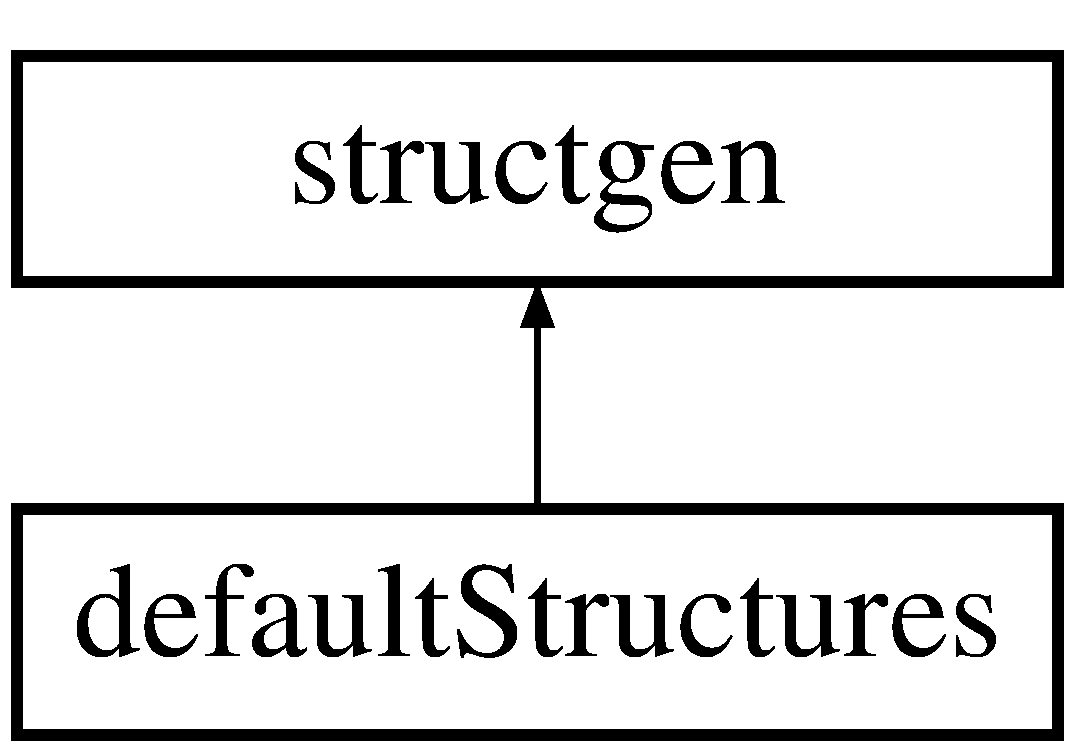
\includegraphics[height=2.000000cm]{classdefault_structures}
\end{center}
\end{figure}
\subsection*{Additional Inherited Members}


\subsection{Detailed Description}


Definition at line 220 of file structure.\-generator.\-structgen.\-php.



The documentation for this class was generated from the following file\-:\begin{DoxyCompactItemize}
\item 
/home/peter/git/\-Open\-Sencillo/fw\-\_\-libraries/structure.\-generator.\-structgen.\-php\end{DoxyCompactItemize}

\hypertarget{classfdel}{\section{fdel Class Reference}
\label{classfdel}\index{fdel@{fdel}}
}
\subsection*{Public Member Functions}
\begin{DoxyCompactItemize}
\item 
\hyperlink{classfdel_af104a08d89a5bbf1f513b65fdc8bba1f}{\-\_\-\-\_\-construct} (\$storage)
\item 
\hyperlink{classfdel_aaed74f7942d3fc56582e99324500e87b}{debug} ()
\item 
\hyperlink{classfdel_a91e316c945c62d9fca01935263815b03}{delete\-File} (\$name)
\item 
\hyperlink{classfdel_acad5a617688373b7d8032baefa0dad1b}{delete\-Folder} (\$name)
\item 
\hyperlink{classfdel_a45176edc5172bdb59f6a1fe0cd2235f4}{delete\-Old\-File} (\$older\-Than=7)
\end{DoxyCompactItemize}
\subsection*{Protected Attributes}
\begin{DoxyCompactItemize}
\item 
\hypertarget{classfdel_a6efc15b5a2314dd4b5aaa556a375c6d6}{{\bfseries \$data}}\label{classfdel_a6efc15b5a2314dd4b5aaa556a375c6d6}

\end{DoxyCompactItemize}


\subsection{Detailed Description}


Definition at line 11 of file files.\-delete.\-fdel.\-php.



\subsection{Constructor \& Destructor Documentation}
\hypertarget{classfdel_af104a08d89a5bbf1f513b65fdc8bba1f}{\index{fdel@{fdel}!\-\_\-\-\_\-construct@{\-\_\-\-\_\-construct}}
\index{\-\_\-\-\_\-construct@{\-\_\-\-\_\-construct}!fdel@{fdel}}
\subsubsection[{\-\_\-\-\_\-construct}]{\setlength{\rightskip}{0pt plus 5cm}\-\_\-\-\_\-construct (
\begin{DoxyParamCaption}
\item[{}]{\$storage}
\end{DoxyParamCaption}
)}}\label{classfdel_af104a08d89a5bbf1f513b65fdc8bba1f}
Construct 
\begin{DoxyParams}[1]{Parameters}
string & {\em \$storage} & \\
\hline
\end{DoxyParams}


Definition at line 19 of file files.\-delete.\-fdel.\-php.



\subsection{Member Function Documentation}
\hypertarget{classfdel_aaed74f7942d3fc56582e99324500e87b}{\index{fdel@{fdel}!debug@{debug}}
\index{debug@{debug}!fdel@{fdel}}
\subsubsection[{debug}]{\setlength{\rightskip}{0pt plus 5cm}debug (
\begin{DoxyParamCaption}
{}
\end{DoxyParamCaption}
)}}\label{classfdel_aaed74f7942d3fc56582e99324500e87b}
Return debug information \begin{DoxyReturn}{Returns}
array 
\end{DoxyReturn}


Definition at line 29 of file files.\-delete.\-fdel.\-php.

\hypertarget{classfdel_a91e316c945c62d9fca01935263815b03}{\index{fdel@{fdel}!delete\-File@{delete\-File}}
\index{delete\-File@{delete\-File}!fdel@{fdel}}
\subsubsection[{delete\-File}]{\setlength{\rightskip}{0pt plus 5cm}delete\-File (
\begin{DoxyParamCaption}
\item[{}]{\$name}
\end{DoxyParamCaption}
)}}\label{classfdel_a91e316c945c62d9fca01935263815b03}
Delete one file 
\begin{DoxyParams}[1]{Parameters}
string & {\em \$name} & \\
\hline
\end{DoxyParams}
\begin{DoxyReturn}{Returns}
boolean 
\end{DoxyReturn}


Definition at line 39 of file files.\-delete.\-fdel.\-php.

\hypertarget{classfdel_acad5a617688373b7d8032baefa0dad1b}{\index{fdel@{fdel}!delete\-Folder@{delete\-Folder}}
\index{delete\-Folder@{delete\-Folder}!fdel@{fdel}}
\subsubsection[{delete\-Folder}]{\setlength{\rightskip}{0pt plus 5cm}delete\-Folder (
\begin{DoxyParamCaption}
\item[{}]{\$name}
\end{DoxyParamCaption}
)}}\label{classfdel_acad5a617688373b7d8032baefa0dad1b}
Delete folder by name 
\begin{DoxyParams}[1]{Parameters}
string & {\em \$name} & \\
\hline
\end{DoxyParams}
\begin{DoxyReturn}{Returns}
boolean 
\end{DoxyReturn}


Definition at line 66 of file files.\-delete.\-fdel.\-php.

\hypertarget{classfdel_a45176edc5172bdb59f6a1fe0cd2235f4}{\index{fdel@{fdel}!delete\-Old\-File@{delete\-Old\-File}}
\index{delete\-Old\-File@{delete\-Old\-File}!fdel@{fdel}}
\subsubsection[{delete\-Old\-File}]{\setlength{\rightskip}{0pt plus 5cm}delete\-Old\-File (
\begin{DoxyParamCaption}
\item[{}]{\$older\-Than = {\ttfamily 7}}
\end{DoxyParamCaption}
)}}\label{classfdel_a45176edc5172bdb59f6a1fe0cd2235f4}
Delete old file by expire day 
\begin{DoxyParams}[1]{Parameters}
number & {\em \$older\-Than} & \\
\hline
\end{DoxyParams}
\begin{DoxyReturn}{Returns}
number 
\end{DoxyReturn}


Definition at line 87 of file files.\-delete.\-fdel.\-php.



The documentation for this class was generated from the following file\-:\begin{DoxyCompactItemize}
\item 
/home/peter/git/\-Open\-Sencillo/fw\-\_\-libraries/files.\-delete.\-fdel.\-php\end{DoxyCompactItemize}

\hypertarget{classfile}{\section{file Class Reference}
\label{classfile}\index{file@{file}}
}
Inheritance diagram for file\-:\begin{figure}[H]
\begin{center}
\leavevmode
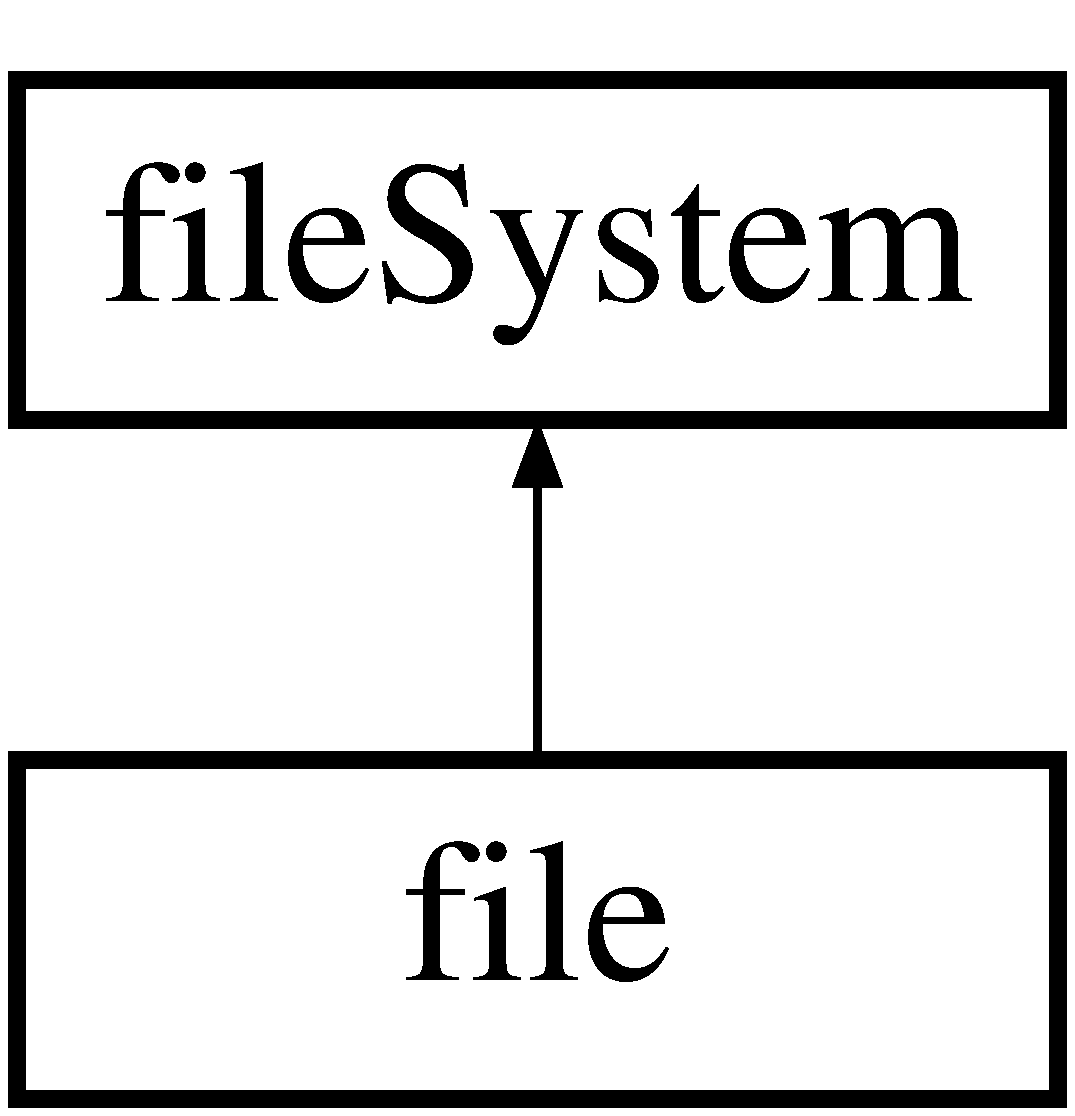
\includegraphics[height=2.000000cm]{classfile}
\end{center}
\end{figure}
\subsection*{Public Member Functions}
\begin{DoxyCompactItemize}
\item 
\hyperlink{classfile_a4717bbfc70a40a57ee741ed70766c309}{\-\_\-\-\_\-construct} (\$name)
\item 
\hyperlink{classfile_a421831a265621325e1fdd19aace0c758}{\-\_\-\-\_\-destruct} ()
\end{DoxyCompactItemize}
\subsection*{Additional Inherited Members}


\subsection{Detailed Description}


Definition at line 62 of file core\-\_\-functions.\-php.



\subsection{Constructor \& Destructor Documentation}
\hypertarget{classfile_a4717bbfc70a40a57ee741ed70766c309}{\index{file@{file}!\-\_\-\-\_\-construct@{\-\_\-\-\_\-construct}}
\index{\-\_\-\-\_\-construct@{\-\_\-\-\_\-construct}!file@{file}}
\subsubsection[{\-\_\-\-\_\-construct}]{\setlength{\rightskip}{0pt plus 5cm}\-\_\-\-\_\-construct (
\begin{DoxyParamCaption}
\item[{}]{\$name}
\end{DoxyParamCaption}
)}}\label{classfile_a4717bbfc70a40a57ee741ed70766c309}
Switch folders chmod to 0777 
\begin{DoxyParams}[1]{Parameters}
string & {\em \$name} & \\
\hline
\end{DoxyParams}


Definition at line 68 of file core\-\_\-functions.\-php.

\hypertarget{classfile_a421831a265621325e1fdd19aace0c758}{\index{file@{file}!\-\_\-\-\_\-destruct@{\-\_\-\-\_\-destruct}}
\index{\-\_\-\-\_\-destruct@{\-\_\-\-\_\-destruct}!file@{file}}
\subsubsection[{\-\_\-\-\_\-destruct}]{\setlength{\rightskip}{0pt plus 5cm}\-\_\-\-\_\-destruct (
\begin{DoxyParamCaption}
{}
\end{DoxyParamCaption}
)}}\label{classfile_a421831a265621325e1fdd19aace0c758}
Switch folders chmod to 0700 
\begin{DoxyParams}[1]{Parameters}
string & {\em \$name} & \\
\hline
\end{DoxyParams}


Definition at line 82 of file core\-\_\-functions.\-php.



The documentation for this class was generated from the following file\-:\begin{DoxyCompactItemize}
\item 
/home/peter/git/\-Open\-Sencillo/fw\-\_\-core/core\-\_\-functions.\-php\end{DoxyCompactItemize}

\hypertarget{classfiles_list}{\section{files\-List Class Reference}
\label{classfiles_list}\index{files\-List@{files\-List}}
}
\subsection*{Public Member Functions}
\begin{DoxyCompactItemize}
\item 
\hypertarget{classfiles_list_a03853ceaa393e487835b287de58aba5a}{{\bfseries \-\_\-\-\_\-construct} (\$path)}\label{classfiles_list_a03853ceaa393e487835b287de58aba5a}

\item 
\hyperlink{classfiles_list_a3593ec13e3e24737585badced66b43e1}{scan\-Dir} (\$dir='./')
\item 
\hyperlink{classfiles_list_a7ccfe88b459f36381d83b8fd039999c8}{find\-Files} (\$dir, \&\$dir\-\_\-array)
\item 
\hyperlink{classfiles_list_ac08cf4a0b3b018e45d7d9eee5f6e1028}{find\-Files\-Structure} (\$dir)
\item 
\hyperlink{classfiles_list_ab39d896ae81da27aff1c1611d2ec221e}{array\-To\-Html} (\$style, \$folder\-Style=null, \$ftypes=null, \$dot=null)
\end{DoxyCompactItemize}
\subsection*{Protected Attributes}
\begin{DoxyCompactItemize}
\item 
\hypertarget{classfiles_list_a0a4baf0b22973c07685c3981f0d17fc4}{{\bfseries \$path}}\label{classfiles_list_a0a4baf0b22973c07685c3981f0d17fc4}

\item 
\hypertarget{classfiles_list_ae6c874521ea9958e89e89f1d4d6e01d5}{{\bfseries \$folderlist}}\label{classfiles_list_ae6c874521ea9958e89e89f1d4d6e01d5}

\end{DoxyCompactItemize}


\subsection{Detailed Description}


Definition at line 11 of file files.\-management.\-fman.\-php.



\subsection{Member Function Documentation}
\hypertarget{classfiles_list_ab39d896ae81da27aff1c1611d2ec221e}{\index{files\-List@{files\-List}!array\-To\-Html@{array\-To\-Html}}
\index{array\-To\-Html@{array\-To\-Html}!filesList@{files\-List}}
\subsubsection[{array\-To\-Html}]{\setlength{\rightskip}{0pt plus 5cm}array\-To\-Html (
\begin{DoxyParamCaption}
\item[{}]{\$style, }
\item[{}]{\$folder\-Style = {\ttfamily null}, }
\item[{}]{\$ftypes = {\ttfamily null}, }
\item[{}]{\$dot = {\ttfamily null}}
\end{DoxyParamCaption}
)}}\label{classfiles_list_ab39d896ae81da27aff1c1611d2ec221e}
Convert array to html list 
\begin{DoxyParams}[1]{Parameters}
array & {\em \$style} & \\
\hline
array & {\em \$folder\-Style} & \\
\hline
bool & {\em \$dot} & \\
\hline
\end{DoxyParams}
\begin{DoxyReturn}{Returns}
string 
\end{DoxyReturn}


Definition at line 115 of file files.\-management.\-fman.\-php.

\hypertarget{classfiles_list_a7ccfe88b459f36381d83b8fd039999c8}{\index{files\-List@{files\-List}!find\-Files@{find\-Files}}
\index{find\-Files@{find\-Files}!filesList@{files\-List}}
\subsubsection[{find\-Files}]{\setlength{\rightskip}{0pt plus 5cm}find\-Files (
\begin{DoxyParamCaption}
\item[{}]{\$dir, }
\item[{\&}]{\$dir\-\_\-array}
\end{DoxyParamCaption}
)}}\label{classfiles_list_a7ccfe88b459f36381d83b8fd039999c8}
Get all files, folders, subfiles and subfolders from directory


\begin{DoxyParams}[1]{Parameters}
string & {\em \$dir} & (path to start directory) \\
\hline
array & {\em \&\$dir\-\_\-array} & (array for update) \\
\hline
\end{DoxyParams}


Definition at line 48 of file files.\-management.\-fman.\-php.

\hypertarget{classfiles_list_ac08cf4a0b3b018e45d7d9eee5f6e1028}{\index{files\-List@{files\-List}!find\-Files\-Structure@{find\-Files\-Structure}}
\index{find\-Files\-Structure@{find\-Files\-Structure}!filesList@{files\-List}}
\subsubsection[{find\-Files\-Structure}]{\setlength{\rightskip}{0pt plus 5cm}find\-Files\-Structure (
\begin{DoxyParamCaption}
\item[{}]{\$dir}
\end{DoxyParamCaption}
)}}\label{classfiles_list_ac08cf4a0b3b018e45d7d9eee5f6e1028}
Scan directory structure and recursive scannig subdirectory structure


\begin{DoxyParams}[1]{Parameters}
string & {\em \$dir} & \\
\hline
\end{DoxyParams}
\begin{DoxyReturn}{Returns}
array 
\end{DoxyReturn}


Definition at line 85 of file files.\-management.\-fman.\-php.

\hypertarget{classfiles_list_a3593ec13e3e24737585badced66b43e1}{\index{files\-List@{files\-List}!scan\-Dir@{scan\-Dir}}
\index{scan\-Dir@{scan\-Dir}!filesList@{files\-List}}
\subsubsection[{scan\-Dir}]{\setlength{\rightskip}{0pt plus 5cm}scan\-Dir (
\begin{DoxyParamCaption}
\item[{}]{\$dir = {\ttfamily './'}}
\end{DoxyParamCaption}
)}}\label{classfiles_list_a3593ec13e3e24737585badced66b43e1}
Create complet file list


\begin{DoxyParams}[1]{Parameters}
string & {\em \$dir} & (path)\\
\hline
\end{DoxyParams}
\begin{DoxyReturn}{Returns}
array 
\end{DoxyReturn}


Definition at line 36 of file files.\-management.\-fman.\-php.



The documentation for this class was generated from the following file\-:\begin{DoxyCompactItemize}
\item 
/home/peter/git/\-Open\-Sencillo/fw\-\_\-libraries/files.\-management.\-fman.\-php\end{DoxyCompactItemize}

\hypertarget{classfile_system}{\section{file\-System Class Reference}
\label{classfile_system}\index{file\-System@{file\-System}}
}
Inheritance diagram for file\-System\-:\begin{figure}[H]
\begin{center}
\leavevmode
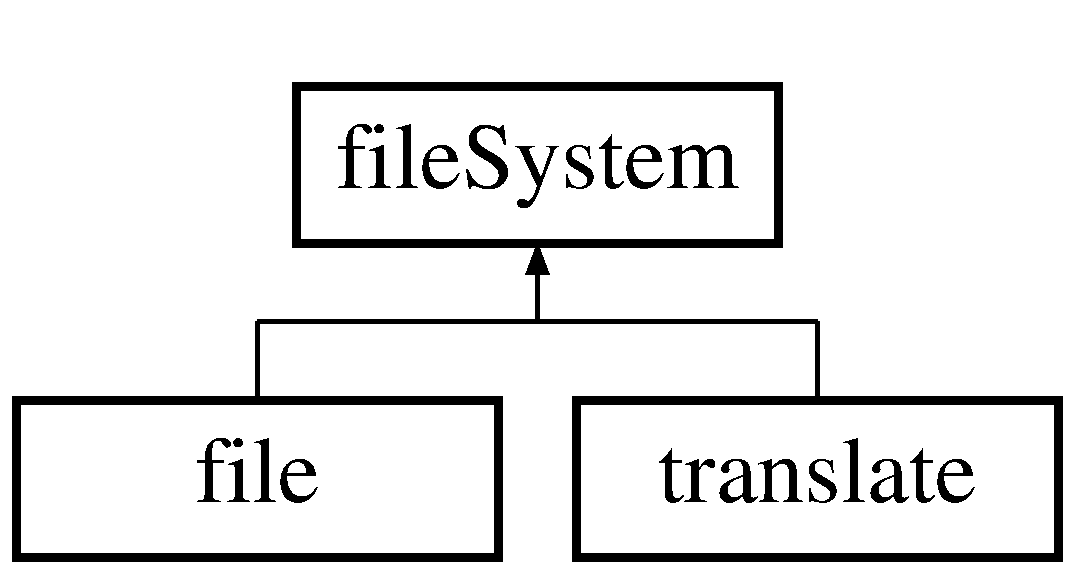
\includegraphics[height=2.000000cm]{classfile_system}
\end{center}
\end{figure}
\subsection*{Public Member Functions}
\begin{DoxyCompactItemize}
\item 
\hyperlink{classfile_system_a4717bbfc70a40a57ee741ed70766c309}{\-\_\-\-\_\-construct} (\$name)
\item 
\hyperlink{classfile_system_a85013b0dcf138f6997e2a05332ed0dd5}{write} (\$data)
\item 
\hyperlink{classfile_system_a64571309bfb3238c65fd3c2898f92440}{read} ()
\end{DoxyCompactItemize}
\subsection*{Data Fields}
\begin{DoxyCompactItemize}
\item 
\hypertarget{classfile_system_ab2fc40d43824ea3e1ce5d86dee0d763b}{{\bfseries \$name}}\label{classfile_system_ab2fc40d43824ea3e1ce5d86dee0d763b}

\end{DoxyCompactItemize}


\subsection{Detailed Description}


Definition at line 11 of file core\-\_\-functions.\-php.



\subsection{Constructor \& Destructor Documentation}
\hypertarget{classfile_system_a4717bbfc70a40a57ee741ed70766c309}{\index{file\-System@{file\-System}!\-\_\-\-\_\-construct@{\-\_\-\-\_\-construct}}
\index{\-\_\-\-\_\-construct@{\-\_\-\-\_\-construct}!fileSystem@{file\-System}}
\subsubsection[{\-\_\-\-\_\-construct}]{\setlength{\rightskip}{0pt plus 5cm}\-\_\-\-\_\-construct (
\begin{DoxyParamCaption}
\item[{}]{\$name}
\end{DoxyParamCaption}
)}}\label{classfile_system_a4717bbfc70a40a57ee741ed70766c309}
\hyperlink{classfile_system}{file\-System} constructor -\/ create object for file manipulation 
\begin{DoxyParams}[1]{Parameters}
string & {\em \$name} & \\
\hline
\end{DoxyParams}


Definition at line 23 of file core\-\_\-functions.\-php.



\subsection{Member Function Documentation}
\hypertarget{classfile_system_a64571309bfb3238c65fd3c2898f92440}{\index{file\-System@{file\-System}!read@{read}}
\index{read@{read}!fileSystem@{file\-System}}
\subsubsection[{read}]{\setlength{\rightskip}{0pt plus 5cm}read (
\begin{DoxyParamCaption}
{}
\end{DoxyParamCaption}
)\hspace{0.3cm}{\ttfamily [final]}}}\label{classfile_system_a64571309bfb3238c65fd3c2898f92440}
Read file from file \begin{DoxyReturn}{Returns}
string 
\end{DoxyReturn}


Definition at line 41 of file core\-\_\-functions.\-php.

\hypertarget{classfile_system_a85013b0dcf138f6997e2a05332ed0dd5}{\index{file\-System@{file\-System}!write@{write}}
\index{write@{write}!fileSystem@{file\-System}}
\subsubsection[{write}]{\setlength{\rightskip}{0pt plus 5cm}write (
\begin{DoxyParamCaption}
\item[{}]{\$data}
\end{DoxyParamCaption}
)\hspace{0.3cm}{\ttfamily [final]}}}\label{classfile_system_a85013b0dcf138f6997e2a05332ed0dd5}
Write data to file 
\begin{DoxyParams}[1]{Parameters}
string & {\em \$data} & to write \\
\hline
\end{DoxyParams}


Definition at line 31 of file core\-\_\-functions.\-php.



The documentation for this class was generated from the following file\-:\begin{DoxyCompactItemize}
\item 
/home/peter/git/\-Open\-Sencillo/fw\-\_\-core/core\-\_\-functions.\-php\end{DoxyCompactItemize}

\hypertarget{classform_creator}{\section{form\-Creator Class Reference}
\label{classform_creator}\index{form\-Creator@{form\-Creator}}
}
\subsection*{Public Member Functions}
\begin{DoxyCompactItemize}
\item 
\hypertarget{classform_creator_af18d37619b90c3eabf6a5d2c59763745}{{\bfseries create} (\$type, \$params)}\label{classform_creator_af18d37619b90c3eabf6a5d2c59763745}

\item 
\hyperlink{classform_creator_ab09542cd5fe8c41321535f2586520e43}{get\-By\-Id} (\$id, \$action=\char`\"{}/\char`\"{}, \$method=\char`\"{}post\char`\"{})
\item 
\hyperlink{classform_creator_aec79743fc2831bef599b86ad0226e7a7}{group\-To\-Lines} (\$id, \$tag=null, \$params=null)
\end{DoxyCompactItemize}
\subsection*{Protected Attributes}
\begin{DoxyCompactItemize}
\item 
\hypertarget{classform_creator_a1a4fda4c28a9ee5f91102c023b9501f4}{{\bfseries \$form} =array()}\label{classform_creator_a1a4fda4c28a9ee5f91102c023b9501f4}

\end{DoxyCompactItemize}


\subsection{Detailed Description}


Definition at line 12 of file form.\-tool.\-framework.\-php.



\subsection{Member Function Documentation}
\hypertarget{classform_creator_ab09542cd5fe8c41321535f2586520e43}{\index{form\-Creator@{form\-Creator}!get\-By\-Id@{get\-By\-Id}}
\index{get\-By\-Id@{get\-By\-Id}!formCreator@{form\-Creator}}
\subsubsection[{get\-By\-Id}]{\setlength{\rightskip}{0pt plus 5cm}get\-By\-Id (
\begin{DoxyParamCaption}
\item[{}]{\$id, }
\item[{}]{\$action = {\ttfamily \char`\"{}/\char`\"{}}, }
\item[{}]{\$method = {\ttfamily \char`\"{}post\char`\"{}}}
\end{DoxyParamCaption}
)}}\label{classform_creator_ab09542cd5fe8c41321535f2586520e43}
Create form


\begin{DoxyParams}[1]{Parameters}
array & {\em \$id} & (identification in the system)\\
\hline
\end{DoxyParams}
\begin{DoxyReturn}{Returns}
string (if exist \$id retruning html input tag) 
\end{DoxyReturn}


Definition at line 79 of file form.\-tool.\-framework.\-php.

\hypertarget{classform_creator_aec79743fc2831bef599b86ad0226e7a7}{\index{form\-Creator@{form\-Creator}!group\-To\-Lines@{group\-To\-Lines}}
\index{group\-To\-Lines@{group\-To\-Lines}!formCreator@{form\-Creator}}
\subsubsection[{group\-To\-Lines}]{\setlength{\rightskip}{0pt plus 5cm}group\-To\-Lines (
\begin{DoxyParamCaption}
\item[{}]{\$id, }
\item[{}]{\$tag = {\ttfamily null}, }
\item[{}]{\$params = {\ttfamily null}}
\end{DoxyParamCaption}
)}}\label{classform_creator_aec79743fc2831bef599b86ad0226e7a7}
Create a new form line (no save)


\begin{DoxyParams}[1]{Parameters}
string & {\em \$id} & \\
\hline
string & {\em \$tag,=null} & \\
\hline
\end{DoxyParams}
\begin{DoxyReturn}{Returns}
string 
\end{DoxyReturn}


Definition at line 98 of file form.\-tool.\-framework.\-php.



The documentation for this class was generated from the following file\-:\begin{DoxyCompactItemize}
\item 
/home/peter/git/\-Open\-Sencillo/fw\-\_\-libraries/form.\-tool.\-framework.\-php\end{DoxyCompactItemize}

\hypertarget{classget_cookies}{\section{get\-Cookies Class Reference}
\label{classget_cookies}\index{get\-Cookies@{get\-Cookies}}
}
\subsection*{Public Member Functions}
\begin{DoxyCompactItemize}
\item 
\hyperlink{classget_cookies_a095c5d389db211932136b53f25f39685}{\-\_\-\-\_\-construct} ()
\item 
\hyperlink{classget_cookies_abc5ed2696aca517e302e8108fd40e5a6}{set\-Expiration} (\$time)
\item 
\hyperlink{classget_cookies_a5eb869c0c92e14a8e642183097d3667d}{add\-Cookie} (\$name, \$data)
\item 
\hyperlink{classget_cookies_a37ad70677fa7dfb0a03eb58bc0eead6d}{remove\-Cookie} (\$name)
\end{DoxyCompactItemize}
\begin{Indent}{\bf string \$name}\par
{\em Get saved cookie by name

\begin{DoxyReturn}{Returns}
mixed 
\end{DoxyReturn}
}\begin{DoxyCompactItemize}
\item 
\hypertarget{classget_cookies_a1c999cd2e8d238603ef9a39a6d5dddb4}{{\bfseries get\-Cookie} (\$name)}\label{classget_cookies_a1c999cd2e8d238603ef9a39a6d5dddb4}

\end{DoxyCompactItemize}
\end{Indent}


\subsection{Detailed Description}


Definition at line 27 of file cookies.\-php.



\subsection{Constructor \& Destructor Documentation}
\hypertarget{classget_cookies_a095c5d389db211932136b53f25f39685}{\index{get\-Cookies@{get\-Cookies}!\-\_\-\-\_\-construct@{\-\_\-\-\_\-construct}}
\index{\-\_\-\-\_\-construct@{\-\_\-\-\_\-construct}!getCookies@{get\-Cookies}}
\subsubsection[{\-\_\-\-\_\-construct}]{\setlength{\rightskip}{0pt plus 5cm}\-\_\-\-\_\-construct (
\begin{DoxyParamCaption}
{}
\end{DoxyParamCaption}
)}}\label{classget_cookies_a095c5d389db211932136b53f25f39685}
Create expiration time 

Definition at line 36 of file cookies.\-php.



\subsection{Member Function Documentation}
\hypertarget{classget_cookies_a5eb869c0c92e14a8e642183097d3667d}{\index{get\-Cookies@{get\-Cookies}!add\-Cookie@{add\-Cookie}}
\index{add\-Cookie@{add\-Cookie}!getCookies@{get\-Cookies}}
\subsubsection[{add\-Cookie}]{\setlength{\rightskip}{0pt plus 5cm}add\-Cookie (
\begin{DoxyParamCaption}
\item[{}]{\$name, }
\item[{}]{\$data}
\end{DoxyParamCaption}
)}}\label{classget_cookies_a5eb869c0c92e14a8e642183097d3667d}
Add cookie 
\begin{DoxyParams}[1]{Parameters}
string & {\em \$name} & \\
\hline
mixed & {\em \$data} & \\
\hline
\end{DoxyParams}


Definition at line 55 of file cookies.\-php.

\hypertarget{classget_cookies_a37ad70677fa7dfb0a03eb58bc0eead6d}{\index{get\-Cookies@{get\-Cookies}!remove\-Cookie@{remove\-Cookie}}
\index{remove\-Cookie@{remove\-Cookie}!getCookies@{get\-Cookies}}
\subsubsection[{remove\-Cookie}]{\setlength{\rightskip}{0pt plus 5cm}remove\-Cookie (
\begin{DoxyParamCaption}
\item[{}]{\$name}
\end{DoxyParamCaption}
)}}\label{classget_cookies_a37ad70677fa7dfb0a03eb58bc0eead6d}
Remove cookie 
\begin{DoxyParams}[1]{Parameters}
string & {\em \$name} & \\
\hline
\end{DoxyParams}


Definition at line 67 of file cookies.\-php.

\hypertarget{classget_cookies_abc5ed2696aca517e302e8108fd40e5a6}{\index{get\-Cookies@{get\-Cookies}!set\-Expiration@{set\-Expiration}}
\index{set\-Expiration@{set\-Expiration}!getCookies@{get\-Cookies}}
\subsubsection[{set\-Expiration}]{\setlength{\rightskip}{0pt plus 5cm}set\-Expiration (
\begin{DoxyParamCaption}
\item[{}]{\$time}
\end{DoxyParamCaption}
)}}\label{classget_cookies_abc5ed2696aca517e302e8108fd40e5a6}
Set expiration time 
\begin{DoxyParams}[1]{Parameters}
integer & {\em \$time} & \\
\hline
\end{DoxyParams}


Definition at line 45 of file cookies.\-php.



The documentation for this class was generated from the following file\-:\begin{DoxyCompactItemize}
\item 
/home/peter/git/\-Open\-Sencillo/fw\-\_\-headers/cookies.\-php\end{DoxyCompactItemize}

\hypertarget{classheader_seo}{\section{header\-Seo Class Reference}
\label{classheader_seo}\index{header\-Seo@{header\-Seo}}
}
\subsection*{Public Member Functions}
\begin{DoxyCompactItemize}
\item 
\hyperlink{classheader_seo_a095c5d389db211932136b53f25f39685}{\-\_\-\-\_\-construct} ()
\item 
\hyperlink{classheader_seo_a6731160af6291e4d9f49bdf99e12eea8}{keywords} (\$kw)
\item 
\hyperlink{classheader_seo_adf0fd8dd948e7622a113218888789b4c}{encode} (\$ec='U\-T\-F-\/8')
\item 
\hyperlink{classheader_seo_abfdce57af88e3f1213816e5e6a6676e9}{responsive} ()
\item 
\hyperlink{classheader_seo_a8a181ec2d8a26ba25144cad400ca3a87}{title} (\$t)
\item 
\hyperlink{classheader_seo_a9ac92a195c29bc1edc1475eef4923c72}{description} (\$data)
\item 
\hyperlink{classheader_seo_a63237197ed5c8199150856dc71ec9e97}{robots} ()
\item 
\hyperlink{classheader_seo_a2dcb21be96d78f504583452f906e8ad1}{owner} (\$author)
\item 
\hyperlink{classheader_seo_a3d46f2f84b0bf0de1921a0cb899bedff}{generator} ()
\item 
\hyperlink{classheader_seo_a61e85615da2625b55b5580d7ec5e9258}{custom} (\$code)
\item 
\hypertarget{classheader_seo_a21fdbf37b0f5c645d980ba7a96fabf6e}{{\bfseries script} (\$code)}\label{classheader_seo_a21fdbf37b0f5c645d980ba7a96fabf6e}

\item 
\hyperlink{classheader_seo_afc8a3c62679cf00ade9f15fb2a6d6132}{save} ()
\item 
\hypertarget{classheader_seo_aa47df0e5b5191e604c711ede952a91fd}{{\bfseries lang} (\$lang)}\label{classheader_seo_aa47df0e5b5191e604c711ede952a91fd}

\item 
\hyperlink{classheader_seo_a7d18829341f798ff00342e4e7d96030a}{google\-Load} ()
\item 
\hyperlink{classheader_seo_a1b6489fdb8d3547f32072eb5a3abd514}{jquery} ()
\item 
\hyperlink{classheader_seo_ac49e736b6e84fc47561fcf0dfe4df35b}{social\-Tags} (\$arr, \$snippet=false)
\item 
\hyperlink{classheader_seo_a861ffee5950974206ca24646eab7d39f}{bootstrap\-Defs} ()
\end{DoxyCompactItemize}
\subsection*{Data Fields}
\begin{DoxyCompactItemize}
\item 
\hypertarget{classheader_seo_a8ec97217cd00453cdb17e5d6a18829ee}{{\bfseries \$seo}}\label{classheader_seo_a8ec97217cd00453cdb17e5d6a18829ee}

\item 
\hypertarget{classheader_seo_ae19722790c6683980bbf0af8572f26ab}{{\bfseries \$info}}\label{classheader_seo_ae19722790c6683980bbf0af8572f26ab}

\end{DoxyCompactItemize}


\subsection{Detailed Description}


Definition at line 102 of file core\-\_\-functions.\-php.



\subsection{Constructor \& Destructor Documentation}
\hypertarget{classheader_seo_a095c5d389db211932136b53f25f39685}{\index{header\-Seo@{header\-Seo}!\-\_\-\-\_\-construct@{\-\_\-\-\_\-construct}}
\index{\-\_\-\-\_\-construct@{\-\_\-\-\_\-construct}!headerSeo@{header\-Seo}}
\subsubsection[{\-\_\-\-\_\-construct}]{\setlength{\rightskip}{0pt plus 5cm}\-\_\-\-\_\-construct (
\begin{DoxyParamCaption}
{}
\end{DoxyParamCaption}
)}}\label{classheader_seo_a095c5d389db211932136b53f25f39685}
Create default status for page 

Definition at line 115 of file core\-\_\-functions.\-php.



\subsection{Member Function Documentation}
\hypertarget{classheader_seo_a861ffee5950974206ca24646eab7d39f}{\index{header\-Seo@{header\-Seo}!bootstrap\-Defs@{bootstrap\-Defs}}
\index{bootstrap\-Defs@{bootstrap\-Defs}!headerSeo@{header\-Seo}}
\subsubsection[{bootstrap\-Defs}]{\setlength{\rightskip}{0pt plus 5cm}bootstrap\-Defs (
\begin{DoxyParamCaption}
{}
\end{DoxyParamCaption}
)}}\label{classheader_seo_a861ffee5950974206ca24646eab7d39f}
Add bootstrap call 

Definition at line 313 of file core\-\_\-functions.\-php.

\hypertarget{classheader_seo_a61e85615da2625b55b5580d7ec5e9258}{\index{header\-Seo@{header\-Seo}!custom@{custom}}
\index{custom@{custom}!headerSeo@{header\-Seo}}
\subsubsection[{custom}]{\setlength{\rightskip}{0pt plus 5cm}custom (
\begin{DoxyParamCaption}
\item[{}]{\$code}
\end{DoxyParamCaption}
)}}\label{classheader_seo_a61e85615da2625b55b5580d7ec5e9258}
Add custom code to header 
\begin{DoxyParams}[1]{Parameters}
string & {\em \$code} & \\
\hline
\end{DoxyParams}


Definition at line 205 of file core\-\_\-functions.\-php.

\hypertarget{classheader_seo_a9ac92a195c29bc1edc1475eef4923c72}{\index{header\-Seo@{header\-Seo}!description@{description}}
\index{description@{description}!headerSeo@{header\-Seo}}
\subsubsection[{description}]{\setlength{\rightskip}{0pt plus 5cm}description (
\begin{DoxyParamCaption}
\item[{}]{\$data}
\end{DoxyParamCaption}
)}}\label{classheader_seo_a9ac92a195c29bc1edc1475eef4923c72}
Page description with max size 159 characters 
\begin{DoxyParams}[1]{Parameters}
string & {\em \$data} & \\
\hline
\end{DoxyParams}


Definition at line 166 of file core\-\_\-functions.\-php.

\hypertarget{classheader_seo_adf0fd8dd948e7622a113218888789b4c}{\index{header\-Seo@{header\-Seo}!encode@{encode}}
\index{encode@{encode}!headerSeo@{header\-Seo}}
\subsubsection[{encode}]{\setlength{\rightskip}{0pt plus 5cm}encode (
\begin{DoxyParamCaption}
\item[{}]{\$ec = {\ttfamily 'UTF-\/8'}}
\end{DoxyParamCaption}
)}}\label{classheader_seo_adf0fd8dd948e7622a113218888789b4c}
Encoding webpage 
\begin{DoxyParams}[1]{Parameters}
string & {\em \$ec} & webpage encoding \\
\hline
\end{DoxyParams}


Definition at line 135 of file core\-\_\-functions.\-php.

\hypertarget{classheader_seo_a3d46f2f84b0bf0de1921a0cb899bedff}{\index{header\-Seo@{header\-Seo}!generator@{generator}}
\index{generator@{generator}!headerSeo@{header\-Seo}}
\subsubsection[{generator}]{\setlength{\rightskip}{0pt plus 5cm}generator (
\begin{DoxyParamCaption}
{}
\end{DoxyParamCaption}
)}}\label{classheader_seo_a3d46f2f84b0bf0de1921a0cb899bedff}
Add page generator meta tag 

Definition at line 196 of file core\-\_\-functions.\-php.

\hypertarget{classheader_seo_a7d18829341f798ff00342e4e7d96030a}{\index{header\-Seo@{header\-Seo}!google\-Load@{google\-Load}}
\index{google\-Load@{google\-Load}!headerSeo@{header\-Seo}}
\subsubsection[{google\-Load}]{\setlength{\rightskip}{0pt plus 5cm}google\-Load (
\begin{DoxyParamCaption}
{}
\end{DoxyParamCaption}
)}}\label{classheader_seo_a7d18829341f798ff00342e4e7d96030a}
Add google load call 

Definition at line 274 of file core\-\_\-functions.\-php.

\hypertarget{classheader_seo_a1b6489fdb8d3547f32072eb5a3abd514}{\index{header\-Seo@{header\-Seo}!jquery@{jquery}}
\index{jquery@{jquery}!headerSeo@{header\-Seo}}
\subsubsection[{jquery}]{\setlength{\rightskip}{0pt plus 5cm}jquery (
\begin{DoxyParamCaption}
{}
\end{DoxyParamCaption}
)}}\label{classheader_seo_a1b6489fdb8d3547f32072eb5a3abd514}
Add jquery 

Definition at line 283 of file core\-\_\-functions.\-php.

\hypertarget{classheader_seo_a6731160af6291e4d9f49bdf99e12eea8}{\index{header\-Seo@{header\-Seo}!keywords@{keywords}}
\index{keywords@{keywords}!headerSeo@{header\-Seo}}
\subsubsection[{keywords}]{\setlength{\rightskip}{0pt plus 5cm}keywords (
\begin{DoxyParamCaption}
\item[{}]{\$kw}
\end{DoxyParamCaption}
)}}\label{classheader_seo_a6731160af6291e4d9f49bdf99e12eea8}
Basic function for generate keywords tag 
\begin{DoxyParams}[1]{Parameters}
string & {\em \$kw} & add keywords \\
\hline
\end{DoxyParams}


Definition at line 126 of file core\-\_\-functions.\-php.

\hypertarget{classheader_seo_a2dcb21be96d78f504583452f906e8ad1}{\index{header\-Seo@{header\-Seo}!owner@{owner}}
\index{owner@{owner}!headerSeo@{header\-Seo}}
\subsubsection[{owner}]{\setlength{\rightskip}{0pt plus 5cm}owner (
\begin{DoxyParamCaption}
\item[{}]{\$author}
\end{DoxyParamCaption}
)}}\label{classheader_seo_a2dcb21be96d78f504583452f906e8ad1}
Add page owner meta tag 
\begin{DoxyParams}[1]{Parameters}
string & {\em \$author} & \\
\hline
\end{DoxyParams}


Definition at line 188 of file core\-\_\-functions.\-php.

\hypertarget{classheader_seo_abfdce57af88e3f1213816e5e6a6676e9}{\index{header\-Seo@{header\-Seo}!responsive@{responsive}}
\index{responsive@{responsive}!headerSeo@{header\-Seo}}
\subsubsection[{responsive}]{\setlength{\rightskip}{0pt plus 5cm}responsive (
\begin{DoxyParamCaption}
{}
\end{DoxyParamCaption}
)}}\label{classheader_seo_abfdce57af88e3f1213816e5e6a6676e9}
Enabled responsive page 

Definition at line 143 of file core\-\_\-functions.\-php.

\hypertarget{classheader_seo_a63237197ed5c8199150856dc71ec9e97}{\index{header\-Seo@{header\-Seo}!robots@{robots}}
\index{robots@{robots}!headerSeo@{header\-Seo}}
\subsubsection[{robots}]{\setlength{\rightskip}{0pt plus 5cm}robots (
\begin{DoxyParamCaption}
{}
\end{DoxyParamCaption}
)}}\label{classheader_seo_a63237197ed5c8199150856dc71ec9e97}
Add settings for Google Bot and Bing Bot 

Definition at line 179 of file core\-\_\-functions.\-php.

\hypertarget{classheader_seo_afc8a3c62679cf00ade9f15fb2a6d6132}{\index{header\-Seo@{header\-Seo}!save@{save}}
\index{save@{save}!headerSeo@{header\-Seo}}
\subsubsection[{save}]{\setlength{\rightskip}{0pt plus 5cm}save (
\begin{DoxyParamCaption}
{}
\end{DoxyParamCaption}
)}}\label{classheader_seo_afc8a3c62679cf00ade9f15fb2a6d6132}
Save S\-E\-O and generate header content \begin{DoxyReturn}{Returns}
string 
\end{DoxyReturn}


Definition at line 224 of file core\-\_\-functions.\-php.

\hypertarget{classheader_seo_ac49e736b6e84fc47561fcf0dfe4df35b}{\index{header\-Seo@{header\-Seo}!social\-Tags@{social\-Tags}}
\index{social\-Tags@{social\-Tags}!headerSeo@{header\-Seo}}
\subsubsection[{social\-Tags}]{\setlength{\rightskip}{0pt plus 5cm}social\-Tags (
\begin{DoxyParamCaption}
\item[{}]{\$arr, }
\item[{}]{\$snippet = {\ttfamily false}}
\end{DoxyParamCaption}
)}}\label{classheader_seo_ac49e736b6e84fc47561fcf0dfe4df35b}
Add og-\/tags and social tags 
\begin{DoxyParams}{Parameters}
{\em array} & \\
\hline
\end{DoxyParams}


Definition at line 292 of file core\-\_\-functions.\-php.

\hypertarget{classheader_seo_a8a181ec2d8a26ba25144cad400ca3a87}{\index{header\-Seo@{header\-Seo}!title@{title}}
\index{title@{title}!headerSeo@{header\-Seo}}
\subsubsection[{title}]{\setlength{\rightskip}{0pt plus 5cm}title (
\begin{DoxyParamCaption}
\item[{}]{\$t}
\end{DoxyParamCaption}
)}}\label{classheader_seo_a8a181ec2d8a26ba25144cad400ca3a87}
Page title 
\begin{DoxyParams}[1]{Parameters}
string & {\em \$t} & title size max 69 characters \\
\hline
\end{DoxyParams}


Definition at line 152 of file core\-\_\-functions.\-php.



The documentation for this class was generated from the following file\-:\begin{DoxyCompactItemize}
\item 
/home/peter/git/\-Open\-Sencillo/fw\-\_\-core/core\-\_\-functions.\-php\end{DoxyCompactItemize}

\hypertarget{classhtgen}{\section{htgen Class Reference}
\label{classhtgen}\index{htgen@{htgen}}
}
\subsection*{Public Member Functions}
\begin{DoxyCompactItemize}
\item 
\hyperlink{classhtgen_a1d6ceb16d5b8ea6fd0e63ed03fde08d6}{cache} (\$type, \$days)
\item 
\hyperlink{classhtgen_a65662d62f9a7f5cd8bb3231aab42d948}{rewrite} (\$status='on', \$base='/', \$port=443)
\item 
\hyperlink{classhtgen_a76ebf2197f307abdb469a204fb24f21d}{pretty\-Url} (\$\hyperlink{classfile}{file}='index.\-php', \$get='p')
\item 
\hyperlink{classhtgen_a0b653c241eea3d479e7db0464956cc6f}{to\-Www} ()
\item 
\hyperlink{classhtgen_a7652afa243aed18054692e9e88a7347b}{prevent\-View} ()
\item 
\hyperlink{classhtgen_aa332281d246627964c36fd68997f98dc}{prevent\-Dir} ()
\item 
\hyperlink{classhtgen_a8acc8015c9cebee7ff40ff3b53f6360b}{directory} (\$dir='index.\-php')
\item 
\hyperlink{classhtgen_a450764950725de9284c7f909799e2c53}{error\-Pages} (\$errpages)
\item 
\hyperlink{classhtgen_a8df2efbc6aa3369c95d10d2347dcc98f}{perm} (\$banlist, \$allowlist=null)
\item 
\hyperlink{classhtgen_a9596f1635d3c078fa06ab0166bcbb11b}{prepare} ()
\item 
\hyperlink{classhtgen_a2a87f7fcb6240f637cceb37d72abc457}{installer\-Scheme} ()
\end{DoxyCompactItemize}
\subsection*{Protected Attributes}
\begin{DoxyCompactItemize}
\item 
\hypertarget{classhtgen_a3fbefca2da7b7d4434ad26f7436c8ff2}{{\bfseries \$gen}}\label{classhtgen_a3fbefca2da7b7d4434ad26f7436c8ff2}

\end{DoxyCompactItemize}


\subsection{Detailed Description}


Definition at line 12 of file htaccess.\-generator.\-htgen.\-php.



\subsection{Member Function Documentation}
\hypertarget{classhtgen_a1d6ceb16d5b8ea6fd0e63ed03fde08d6}{\index{htgen@{htgen}!cache@{cache}}
\index{cache@{cache}!htgen@{htgen}}
\subsubsection[{cache}]{\setlength{\rightskip}{0pt plus 5cm}cache (
\begin{DoxyParamCaption}
\item[{}]{\$type, }
\item[{}]{\$days}
\end{DoxyParamCaption}
)}}\label{classhtgen_a1d6ceb16d5b8ea6fd0e63ed03fde08d6}
H\-T\-A\-C\-C\-E\-S\-S Cache 
\begin{DoxyParams}{Parameters}
{\em string} & mimetype \\
\hline
{\em int} & days \\
\hline
\end{DoxyParams}
\begin{DoxyReturn}{Returns}
array 
\end{DoxyReturn}


Definition at line 21 of file htaccess.\-generator.\-htgen.\-php.

\hypertarget{classhtgen_a8acc8015c9cebee7ff40ff3b53f6360b}{\index{htgen@{htgen}!directory@{directory}}
\index{directory@{directory}!htgen@{htgen}}
\subsubsection[{directory}]{\setlength{\rightskip}{0pt plus 5cm}directory (
\begin{DoxyParamCaption}
\item[{}]{\$dir = {\ttfamily 'index.php'}}
\end{DoxyParamCaption}
)}}\label{classhtgen_a8acc8015c9cebee7ff40ff3b53f6360b}
Change default directory page 
\begin{DoxyParams}{Parameters}
{\em string} & \\
\hline
\end{DoxyParams}
\begin{DoxyReturn}{Returns}
array 
\end{DoxyReturn}


Definition at line 133 of file htaccess.\-generator.\-htgen.\-php.

\hypertarget{classhtgen_a450764950725de9284c7f909799e2c53}{\index{htgen@{htgen}!error\-Pages@{error\-Pages}}
\index{error\-Pages@{error\-Pages}!htgen@{htgen}}
\subsubsection[{error\-Pages}]{\setlength{\rightskip}{0pt plus 5cm}error\-Pages (
\begin{DoxyParamCaption}
\item[{}]{\$errpages}
\end{DoxyParamCaption}
)}}\label{classhtgen_a450764950725de9284c7f909799e2c53}
Error pages path 
\begin{DoxyParams}{Parameters}
{\em array} & error pages paths \\
\hline
\end{DoxyParams}
\begin{DoxyReturn}{Returns}
array 
\end{DoxyReturn}


Definition at line 148 of file htaccess.\-generator.\-htgen.\-php.

\hypertarget{classhtgen_a2a87f7fcb6240f637cceb37d72abc457}{\index{htgen@{htgen}!installer\-Scheme@{installer\-Scheme}}
\index{installer\-Scheme@{installer\-Scheme}!htgen@{htgen}}
\subsubsection[{installer\-Scheme}]{\setlength{\rightskip}{0pt plus 5cm}installer\-Scheme (
\begin{DoxyParamCaption}
{}
\end{DoxyParamCaption}
)}}\label{classhtgen_a2a87f7fcb6240f637cceb37d72abc457}
Default htaccess configuration 

Definition at line 206 of file htaccess.\-generator.\-htgen.\-php.

\hypertarget{classhtgen_a8df2efbc6aa3369c95d10d2347dcc98f}{\index{htgen@{htgen}!perm@{perm}}
\index{perm@{perm}!htgen@{htgen}}
\subsubsection[{perm}]{\setlength{\rightskip}{0pt plus 5cm}perm (
\begin{DoxyParamCaption}
\item[{}]{\$banlist, }
\item[{}]{\$allowlist = {\ttfamily null}}
\end{DoxyParamCaption}
)}}\label{classhtgen_a8df2efbc6aa3369c95d10d2347dcc98f}
Block/\-Allow users by I\-P 
\begin{DoxyParams}{Parameters}
{\em array} & banned ip \\
\hline
{\em array} & allowed ip \\
\hline
\end{DoxyParams}
\begin{DoxyReturn}{Returns}
array 
\end{DoxyReturn}


Definition at line 167 of file htaccess.\-generator.\-htgen.\-php.

\hypertarget{classhtgen_a9596f1635d3c078fa06ab0166bcbb11b}{\index{htgen@{htgen}!prepare@{prepare}}
\index{prepare@{prepare}!htgen@{htgen}}
\subsubsection[{prepare}]{\setlength{\rightskip}{0pt plus 5cm}prepare (
\begin{DoxyParamCaption}
{}
\end{DoxyParamCaption}
)}}\label{classhtgen_a9596f1635d3c078fa06ab0166bcbb11b}
Switch generator to write noarray output mode \begin{DoxyReturn}{Returns}
string 
\end{DoxyReturn}


Definition at line 193 of file htaccess.\-generator.\-htgen.\-php.

\hypertarget{classhtgen_a76ebf2197f307abdb469a204fb24f21d}{\index{htgen@{htgen}!pretty\-Url@{pretty\-Url}}
\index{pretty\-Url@{pretty\-Url}!htgen@{htgen}}
\subsubsection[{pretty\-Url}]{\setlength{\rightskip}{0pt plus 5cm}pretty\-Url (
\begin{DoxyParamCaption}
\item[{}]{\$file = {\ttfamily 'index.php'}, }
\item[{}]{\$get = {\ttfamily 'p'}}
\end{DoxyParamCaption}
)}}\label{classhtgen_a76ebf2197f307abdb469a204fb24f21d}
Create pretty urls format 
\begin{DoxyParams}{Parameters}
{\em string} & requested file name \\
\hline
{\em string} & url get variable \\
\hline
\end{DoxyParams}
\begin{DoxyReturn}{Returns}
array 
\end{DoxyReturn}


Definition at line 69 of file htaccess.\-generator.\-htgen.\-php.

\hypertarget{classhtgen_aa332281d246627964c36fd68997f98dc}{\index{htgen@{htgen}!prevent\-Dir@{prevent\-Dir}}
\index{prevent\-Dir@{prevent\-Dir}!htgen@{htgen}}
\subsubsection[{prevent\-Dir}]{\setlength{\rightskip}{0pt plus 5cm}prevent\-Dir (
\begin{DoxyParamCaption}
{}
\end{DoxyParamCaption}
)}}\label{classhtgen_aa332281d246627964c36fd68997f98dc}
Prevent directory listings \begin{DoxyReturn}{Returns}
array 
\end{DoxyReturn}


Definition at line 118 of file htaccess.\-generator.\-htgen.\-php.

\hypertarget{classhtgen_a7652afa243aed18054692e9e88a7347b}{\index{htgen@{htgen}!prevent\-View@{prevent\-View}}
\index{prevent\-View@{prevent\-View}!htgen@{htgen}}
\subsubsection[{prevent\-View}]{\setlength{\rightskip}{0pt plus 5cm}prevent\-View (
\begin{DoxyParamCaption}
{}
\end{DoxyParamCaption}
)}}\label{classhtgen_a7652afa243aed18054692e9e88a7347b}
Hide htaccess \begin{DoxyReturn}{Returns}
array 
\end{DoxyReturn}


Definition at line 101 of file htaccess.\-generator.\-htgen.\-php.

\hypertarget{classhtgen_a65662d62f9a7f5cd8bb3231aab42d948}{\index{htgen@{htgen}!rewrite@{rewrite}}
\index{rewrite@{rewrite}!htgen@{htgen}}
\subsubsection[{rewrite}]{\setlength{\rightskip}{0pt plus 5cm}rewrite (
\begin{DoxyParamCaption}
\item[{}]{\$status = {\ttfamily 'on'}, }
\item[{}]{\$base = {\ttfamily '/'}, }
\item[{}]{\$port = {\ttfamily 443}}
\end{DoxyParamCaption}
)}}\label{classhtgen_a65662d62f9a7f5cd8bb3231aab42d948}
Create mod\-\_\-rewrite configuration 
\begin{DoxyParams}{Parameters}
{\em string} & on$\vert$off \\
\hline
{\em string} & path example\-: / \\
\hline
{\em int} & page port \\
\hline
\end{DoxyParams}
\begin{DoxyReturn}{Returns}
array 
\end{DoxyReturn}


Definition at line 48 of file htaccess.\-generator.\-htgen.\-php.

\hypertarget{classhtgen_a0b653c241eea3d479e7db0464956cc6f}{\index{htgen@{htgen}!to\-Www@{to\-Www}}
\index{to\-Www@{to\-Www}!htgen@{htgen}}
\subsubsection[{to\-Www}]{\setlength{\rightskip}{0pt plus 5cm}to\-Www (
\begin{DoxyParamCaption}
{}
\end{DoxyParamCaption}
)}}\label{classhtgen_a0b653c241eea3d479e7db0464956cc6f}
Create relocation page opensencillo.\-com -\/$>$ www.\-opensencillo.\-com \begin{DoxyReturn}{Returns}
array 
\end{DoxyReturn}


Definition at line 86 of file htaccess.\-generator.\-htgen.\-php.



The documentation for this class was generated from the following file\-:\begin{DoxyCompactItemize}
\item 
/home/peter/git/\-Open\-Sencillo/fw\-\_\-libraries/htaccess.\-generator.\-htgen.\-php\end{DoxyCompactItemize}

\hypertarget{classinput_rewrite}{\section{input\-Rewrite Class Reference}
\label{classinput_rewrite}\index{input\-Rewrite@{input\-Rewrite}}
}
\subsection*{Public Member Functions}
\begin{DoxyCompactItemize}
\item 
\hyperlink{classinput_rewrite_a1196e18ff5eb24e576a1f9043c5bdcf7}{dot\-Var} (\$source)
\end{DoxyCompactItemize}
\subsection*{Protected Member Functions}
\begin{DoxyCompactItemize}
\item 
\hyperlink{classinput_rewrite_a04e2dd5b1aa7de4db0d0e79ab0264162}{rewrite\-Data} (\$source, \$illegal, \$change)
\item 
\hyperlink{classinput_rewrite_a2baa55b586a3cb2382a89588b5bff5f4}{parse\-Float} (\$pt\-String)
\end{DoxyCompactItemize}


\subsection{Detailed Description}


Definition at line 9 of file input.\-rewrite.\-inrew.\-php.



\subsection{Member Function Documentation}
\hypertarget{classinput_rewrite_a1196e18ff5eb24e576a1f9043c5bdcf7}{\index{input\-Rewrite@{input\-Rewrite}!dot\-Var@{dot\-Var}}
\index{dot\-Var@{dot\-Var}!inputRewrite@{input\-Rewrite}}
\subsubsection[{dot\-Var}]{\setlength{\rightskip}{0pt plus 5cm}dot\-Var (
\begin{DoxyParamCaption}
\item[{}]{\$source}
\end{DoxyParamCaption}
)}}\label{classinput_rewrite_a1196e18ff5eb24e576a1f9043c5bdcf7}
Parse value to float 
\begin{DoxyParams}{Parameters}
{\em \$source} & float $\vert$ string $\vert$ integer \\
\hline
\end{DoxyParams}
\begin{DoxyReturn}{Returns}
float 
\end{DoxyReturn}


Definition at line 30 of file input.\-rewrite.\-inrew.\-php.

\hypertarget{classinput_rewrite_a2baa55b586a3cb2382a89588b5bff5f4}{\index{input\-Rewrite@{input\-Rewrite}!parse\-Float@{parse\-Float}}
\index{parse\-Float@{parse\-Float}!inputRewrite@{input\-Rewrite}}
\subsubsection[{parse\-Float}]{\setlength{\rightskip}{0pt plus 5cm}parse\-Float (
\begin{DoxyParamCaption}
\item[{}]{\$pt\-String}
\end{DoxyParamCaption}
)\hspace{0.3cm}{\ttfamily [protected]}}}\label{classinput_rewrite_a2baa55b586a3cb2382a89588b5bff5f4}
Parse to float 
\begin{DoxyParams}{Parameters}
{\em \$pt\-String} & string \\
\hline
\end{DoxyParams}
\begin{DoxyReturn}{Returns}
float 
\end{DoxyReturn}


Definition at line 40 of file input.\-rewrite.\-inrew.\-php.

\hypertarget{classinput_rewrite_a04e2dd5b1aa7de4db0d0e79ab0264162}{\index{input\-Rewrite@{input\-Rewrite}!rewrite\-Data@{rewrite\-Data}}
\index{rewrite\-Data@{rewrite\-Data}!inputRewrite@{input\-Rewrite}}
\subsubsection[{rewrite\-Data}]{\setlength{\rightskip}{0pt plus 5cm}rewrite\-Data (
\begin{DoxyParamCaption}
\item[{}]{\$source, }
\item[{}]{\$illegal, }
\item[{}]{\$change}
\end{DoxyParamCaption}
)\hspace{0.3cm}{\ttfamily [protected]}}}\label{classinput_rewrite_a04e2dd5b1aa7de4db0d0e79ab0264162}
Basic replace function 
\begin{DoxyParams}{Parameters}
{\em \$source} & array \\
\hline
{\em \$illegal} & array $\vert$ string \\
\hline
{\em \$change} & array $\vert$ string \\
\hline
\end{DoxyParams}
\begin{DoxyReturn}{Returns}
array 
\end{DoxyReturn}


Definition at line 18 of file input.\-rewrite.\-inrew.\-php.



The documentation for this class was generated from the following file\-:\begin{DoxyCompactItemize}
\item 
/home/peter/git/\-Open\-Sencillo/fw\-\_\-libraries/input.\-rewrite.\-inrew.\-php\end{DoxyCompactItemize}

\hypertarget{classlibrary}{\section{library Class Reference}
\label{classlibrary}\index{library@{library}}
}
\subsection*{Public Member Functions}
\begin{DoxyCompactItemize}
\item 
\hyperlink{classlibrary_af8fa59992209e36dccb3eefb0f75531f}{start} ()
\item 
\hyperlink{classlibrary_a06412eb3b5af8cd7d978ac6eab667fbf}{export} ()
\item 
\hyperlink{classlibrary_a19e49aea71e41a8bd6076bc45169e4a3}{status} ()
\item 
\hyperlink{classlibrary_a2e30710ad967fb842b8cc42452bb4e5e}{export\-Path} ()
\end{DoxyCompactItemize}
\subsection*{Data Fields}
\begin{DoxyCompactItemize}
\item 
\hypertarget{classlibrary_a430f5ed50a4c2f3d6ddee6b54bc97eaa}{{\bfseries \$lib}}\label{classlibrary_a430f5ed50a4c2f3d6ddee6b54bc97eaa}

\end{DoxyCompactItemize}
\subsection*{Protected Attributes}
\begin{DoxyCompactItemize}
\item 
\hypertarget{classlibrary_ad2203e5674ffbd18d3fdbcf2cac19a38}{{\bfseries \$all\-\_\-data\-\_\-sencillo}}\label{classlibrary_ad2203e5674ffbd18d3fdbcf2cac19a38}

\item 
\hypertarget{classlibrary_aa1dfa8c07233f1a9171882cc98fd0e2f}{{\bfseries \$readsql}}\label{classlibrary_aa1dfa8c07233f1a9171882cc98fd0e2f}

\item 
\hypertarget{classlibrary_a9590b15215a21e9b42eb546aeef79704}{{\bfseries \$files}}\label{classlibrary_a9590b15215a21e9b42eb546aeef79704}

\item 
\hypertarget{classlibrary_a19e625c76c6796e995f33d323ee3aa84}{{\bfseries \$modules}}\label{classlibrary_a19e625c76c6796e995f33d323ee3aa84}

\end{DoxyCompactItemize}


\subsection{Detailed Description}


Definition at line 11 of file lib\-\_\-identificator.\-php.



\subsection{Member Function Documentation}
\hypertarget{classlibrary_a06412eb3b5af8cd7d978ac6eab667fbf}{\index{library@{library}!export@{export}}
\index{export@{export}!library@{library}}
\subsubsection[{export}]{\setlength{\rightskip}{0pt plus 5cm}export (
\begin{DoxyParamCaption}
{}
\end{DoxyParamCaption}
)}}\label{classlibrary_a06412eb3b5af8cd7d978ac6eab667fbf}
Export data obtained after main proces \begin{DoxyReturn}{Returns}
mixed \mbox{[}(left/right/center/foot/admin)\mbox{]} $\vert$$\vert$ \mbox{[}(numeric value)\mbox{]} 
\end{DoxyReturn}


Definition at line 126 of file lib\-\_\-identificator.\-php.

\hypertarget{classlibrary_a2e30710ad967fb842b8cc42452bb4e5e}{\index{library@{library}!export\-Path@{export\-Path}}
\index{export\-Path@{export\-Path}!library@{library}}
\subsubsection[{export\-Path}]{\setlength{\rightskip}{0pt plus 5cm}export\-Path (
\begin{DoxyParamCaption}
{}
\end{DoxyParamCaption}
)}}\label{classlibrary_a2e30710ad967fb842b8cc42452bb4e5e}
Return array with unique path for class loader \begin{DoxyReturn}{Returns}
arrray 
\end{DoxyReturn}


Definition at line 144 of file lib\-\_\-identificator.\-php.

\hypertarget{classlibrary_af8fa59992209e36dccb3eefb0f75531f}{\index{library@{library}!start@{start}}
\index{start@{start}!library@{library}}
\subsubsection[{start}]{\setlength{\rightskip}{0pt plus 5cm}start (
\begin{DoxyParamCaption}
{}
\end{DoxyParamCaption}
)}}\label{classlibrary_af8fa59992209e36dccb3eefb0f75531f}
Start main mod\-\_\-id proces 

Definition at line 115 of file lib\-\_\-identificator.\-php.

\hypertarget{classlibrary_a19e49aea71e41a8bd6076bc45169e4a3}{\index{library@{library}!status@{status}}
\index{status@{status}!library@{library}}
\subsubsection[{status}]{\setlength{\rightskip}{0pt plus 5cm}status (
\begin{DoxyParamCaption}
{}
\end{DoxyParamCaption}
)}}\label{classlibrary_a19e49aea71e41a8bd6076bc45169e4a3}
Export informations about libraries \begin{DoxyReturn}{Returns}
array 
\end{DoxyReturn}


Definition at line 135 of file lib\-\_\-identificator.\-php.



The documentation for this class was generated from the following file\-:\begin{DoxyCompactItemize}
\item 
/home/peter/git/\-Open\-Sencillo/fw\-\_\-libraries/lib\-\_\-identificator.\-php\end{DoxyCompactItemize}

\hypertarget{classlog}{\section{log Class Reference}
\label{classlog}\index{log@{log}}
}
Inheritance diagram for log\-:\begin{figure}[H]
\begin{center}
\leavevmode
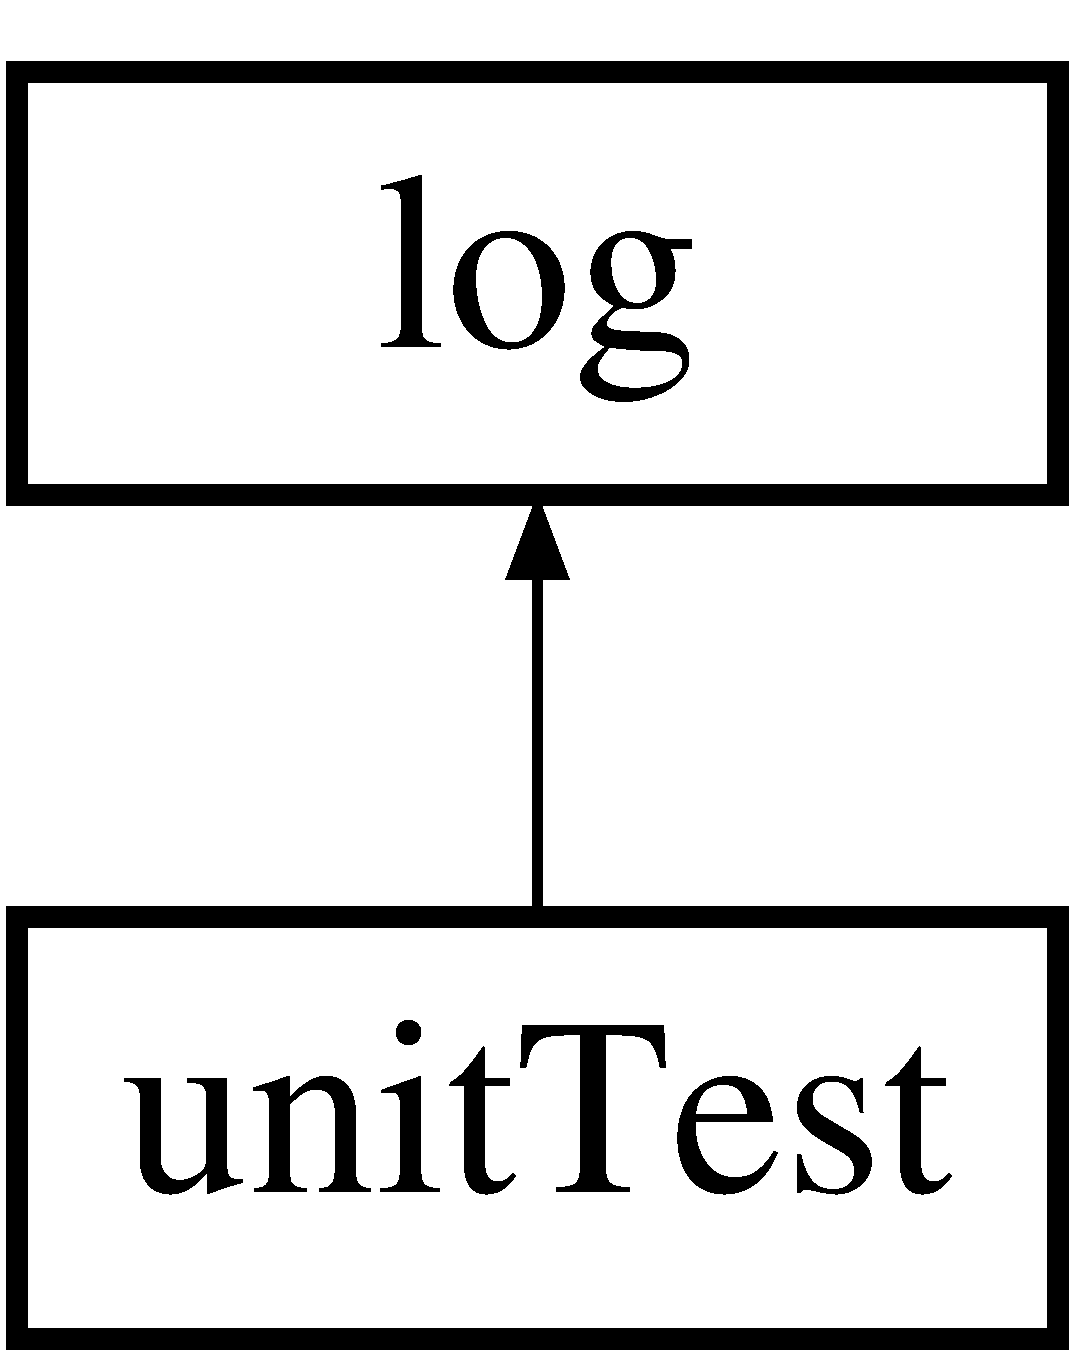
\includegraphics[height=2.000000cm]{classlog}
\end{center}
\end{figure}
\subsection*{Public Member Functions}
\begin{DoxyCompactItemize}
\item 
\hyperlink{classlog_a8e1fbdd4def82189306a52735bd0c70a}{\-\_\-\-\_\-construct} (\$path='', \$\hyperlink{classfile}{file}='log.\-txt', \$max\-Line=100, \$use\-File=true, \$\hyperlink{classmysql}{mysql}=null)
\item 
\hyperlink{classlog_ac4cd1cd9ecb5bdcbf0abfe30f276c430}{save\-To\-Log} (\$data)
\item 
\hyperlink{classlog_af8283af3e7c972d9c276dc634eec0bdc}{get\-Log} ()
\item 
\hyperlink{classlog_ae34a906558f554ea9f61bb2f8f355191}{vd} (\$var)
\end{DoxyCompactItemize}
\subsection*{Protected Attributes}
\begin{DoxyCompactItemize}
\item 
\hypertarget{classlog_ab2fc40d43824ea3e1ce5d86dee0d763b}{{\bfseries \$name}}\label{classlog_ab2fc40d43824ea3e1ce5d86dee0d763b}

\item 
\hypertarget{classlog_aa1bfbd27060176201b271918dff57e8f}{{\bfseries \$file}}\label{classlog_aa1bfbd27060176201b271918dff57e8f}

\item 
\hypertarget{classlog_a0a4baf0b22973c07685c3981f0d17fc4}{{\bfseries \$path}}\label{classlog_a0a4baf0b22973c07685c3981f0d17fc4}

\item 
\hypertarget{classlog_a2c4c58e377f6c66ca38c8ea97666fc5e}{{\bfseries \$current}}\label{classlog_a2c4c58e377f6c66ca38c8ea97666fc5e}

\item 
\hypertarget{classlog_a827b42f70d98e1bf51ff54dbbe771421}{{\bfseries \$store} =array()}\label{classlog_a827b42f70d98e1bf51ff54dbbe771421}

\item 
\hypertarget{classlog_afae5850468ea69a528a75f3b18baae68}{{\bfseries \$max\-Line} =0}\label{classlog_afae5850468ea69a528a75f3b18baae68}

\item 
\hypertarget{classlog_a9900990865c5a574470a0d9886825c56}{{\bfseries \$use\-File}}\label{classlog_a9900990865c5a574470a0d9886825c56}

\end{DoxyCompactItemize}


\subsection{Detailed Description}


Definition at line 11 of file test.\-tool.\-framework.\-php.



\subsection{Constructor \& Destructor Documentation}
\hypertarget{classlog_a8e1fbdd4def82189306a52735bd0c70a}{\index{log@{log}!\-\_\-\-\_\-construct@{\-\_\-\-\_\-construct}}
\index{\-\_\-\-\_\-construct@{\-\_\-\-\_\-construct}!log@{log}}
\subsubsection[{\-\_\-\-\_\-construct}]{\setlength{\rightskip}{0pt plus 5cm}\-\_\-\-\_\-construct (
\begin{DoxyParamCaption}
\item[{}]{\$path = {\ttfamily ''}, }
\item[{}]{\$file = {\ttfamily 'log.txt'}, }
\item[{}]{\$max\-Line = {\ttfamily 100}, }
\item[{}]{\$use\-File = {\ttfamily true}, }
\item[{}]{\$mysql = {\ttfamily null}}
\end{DoxyParamCaption}
)\hspace{0.3cm}{\ttfamily [final]}}}\label{classlog_a8e1fbdd4def82189306a52735bd0c70a}

\begin{DoxyParams}[1]{Parameters}
string & {\em \$path} & \\
\hline
string & {\em \$file} & \\
\hline
number & {\em \$max\-Line} & \\
\hline
bool & {\em \$use\-File} & \\
\hline
\end{DoxyParams}


Definition at line 27 of file test.\-tool.\-framework.\-php.



\subsection{Member Function Documentation}
\hypertarget{classlog_af8283af3e7c972d9c276dc634eec0bdc}{\index{log@{log}!get\-Log@{get\-Log}}
\index{get\-Log@{get\-Log}!log@{log}}
\subsubsection[{get\-Log}]{\setlength{\rightskip}{0pt plus 5cm}get\-Log (
\begin{DoxyParamCaption}
{}
\end{DoxyParamCaption}
)}}\label{classlog_af8283af3e7c972d9c276dc634eec0bdc}
Load from log \begin{DoxyReturn}{Returns}
array 
\end{DoxyReturn}


Definition at line 100 of file test.\-tool.\-framework.\-php.

\hypertarget{classlog_ac4cd1cd9ecb5bdcbf0abfe30f276c430}{\index{log@{log}!save\-To\-Log@{save\-To\-Log}}
\index{save\-To\-Log@{save\-To\-Log}!log@{log}}
\subsubsection[{save\-To\-Log}]{\setlength{\rightskip}{0pt plus 5cm}save\-To\-Log (
\begin{DoxyParamCaption}
\item[{}]{\$data}
\end{DoxyParamCaption}
)\hspace{0.3cm}{\ttfamily [final]}}}\label{classlog_ac4cd1cd9ecb5bdcbf0abfe30f276c430}
Save to log 
\begin{DoxyParams}[1]{Parameters}
string & {\em \$data} & \\
\hline
\end{DoxyParams}


Definition at line 41 of file test.\-tool.\-framework.\-php.

\hypertarget{classlog_ae34a906558f554ea9f61bb2f8f355191}{\index{log@{log}!vd@{vd}}
\index{vd@{vd}!log@{log}}
\subsubsection[{vd}]{\setlength{\rightskip}{0pt plus 5cm}vd (
\begin{DoxyParamCaption}
\item[{}]{\$var}
\end{DoxyParamCaption}
)}}\label{classlog_ae34a906558f554ea9f61bb2f8f355191}
Get formated var\-\_\-dump to string 

Definition at line 109 of file test.\-tool.\-framework.\-php.



The documentation for this class was generated from the following file\-:\begin{DoxyCompactItemize}
\item 
/home/peter/git/\-Open\-Sencillo/fw\-\_\-libraries/test.\-tool.\-framework.\-php\end{DoxyCompactItemize}

\hypertarget{classlogin_manager}{\section{login\-Manager Class Reference}
\label{classlogin_manager}\index{login\-Manager@{login\-Manager}}
}
Inheritance diagram for login\-Manager\-:\begin{figure}[H]
\begin{center}
\leavevmode
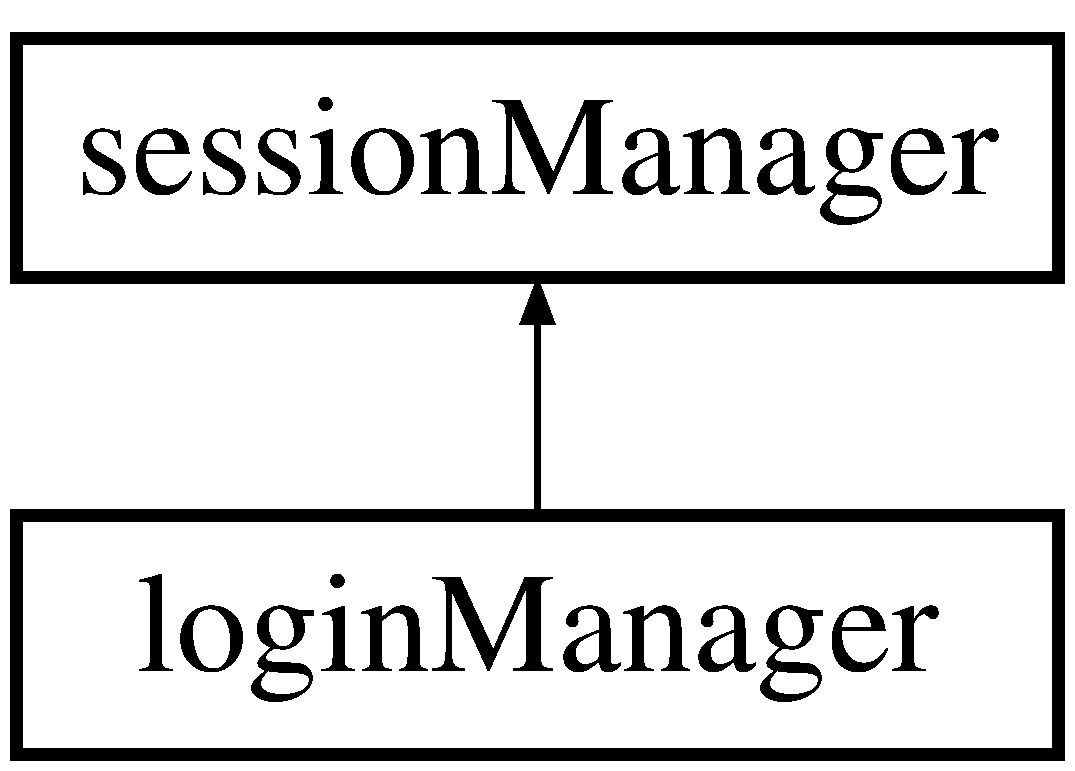
\includegraphics[height=2.000000cm]{classlogin_manager}
\end{center}
\end{figure}
\subsection*{Public Member Functions}
\begin{DoxyCompactItemize}
\item 
\hyperlink{classlogin_manager_a095c5d389db211932136b53f25f39685}{\-\_\-\-\_\-construct} ()
\item 
\hyperlink{classlogin_manager_ad9c5d445e3844daf6a3547c192b14196}{lm\-\_\-install} ()
\item 
\hyperlink{classlogin_manager_a5c8c1321d130f39bede4104c968557e7}{lm\-\_\-add\-User} (\$name, \$pass, \$perm=1000)
\end{DoxyCompactItemize}


\subsection{Detailed Description}


Definition at line 82 of file session.\-php.



\subsection{Constructor \& Destructor Documentation}
\hypertarget{classlogin_manager_a095c5d389db211932136b53f25f39685}{\index{login\-Manager@{login\-Manager}!\-\_\-\-\_\-construct@{\-\_\-\-\_\-construct}}
\index{\-\_\-\-\_\-construct@{\-\_\-\-\_\-construct}!loginManager@{login\-Manager}}
\subsubsection[{\-\_\-\-\_\-construct}]{\setlength{\rightskip}{0pt plus 5cm}\-\_\-\-\_\-construct (
\begin{DoxyParamCaption}
{}
\end{DoxyParamCaption}
)}}\label{classlogin_manager_a095c5d389db211932136b53f25f39685}
Create time settings for \hyperlink{classlogin_manager}{login\-Manager} 

Definition at line 90 of file session.\-php.



\subsection{Member Function Documentation}
\hypertarget{classlogin_manager_a5c8c1321d130f39bede4104c968557e7}{\index{login\-Manager@{login\-Manager}!lm\-\_\-add\-User@{lm\-\_\-add\-User}}
\index{lm\-\_\-add\-User@{lm\-\_\-add\-User}!loginManager@{login\-Manager}}
\subsubsection[{lm\-\_\-add\-User}]{\setlength{\rightskip}{0pt plus 5cm}lm\-\_\-add\-User (
\begin{DoxyParamCaption}
\item[{}]{\$name, }
\item[{}]{\$pass, }
\item[{}]{\$perm = {\ttfamily 1000}}
\end{DoxyParamCaption}
)}}\label{classlogin_manager_a5c8c1321d130f39bede4104c968557e7}
Add user 
\begin{DoxyParams}[1]{Parameters}
string & {\em \$name} & \\
\hline
string & {\em \$pass} & \\
\hline
integer & {\em \$perm} & \\
\hline
\end{DoxyParams}


Definition at line 137 of file session.\-php.

\hypertarget{classlogin_manager_ad9c5d445e3844daf6a3547c192b14196}{\index{login\-Manager@{login\-Manager}!lm\-\_\-install@{lm\-\_\-install}}
\index{lm\-\_\-install@{lm\-\_\-install}!loginManager@{login\-Manager}}
\subsubsection[{lm\-\_\-install}]{\setlength{\rightskip}{0pt plus 5cm}lm\-\_\-install (
\begin{DoxyParamCaption}
{}
\end{DoxyParamCaption}
)}}\label{classlogin_manager_ad9c5d445e3844daf6a3547c192b14196}
Install \hyperlink{classlogin_manager}{login\-Manager} class 

Definition at line 104 of file session.\-php.



The documentation for this class was generated from the following file\-:\begin{DoxyCompactItemize}
\item 
/home/peter/git/\-Open\-Sencillo/fw\-\_\-headers/session.\-php\end{DoxyCompactItemize}

\hypertarget{classlog_man}{\section{log\-Man Class Reference}
\label{classlog_man}\index{log\-Man@{log\-Man}}
}
Inheritance diagram for log\-Man\-:\begin{figure}[H]
\begin{center}
\leavevmode
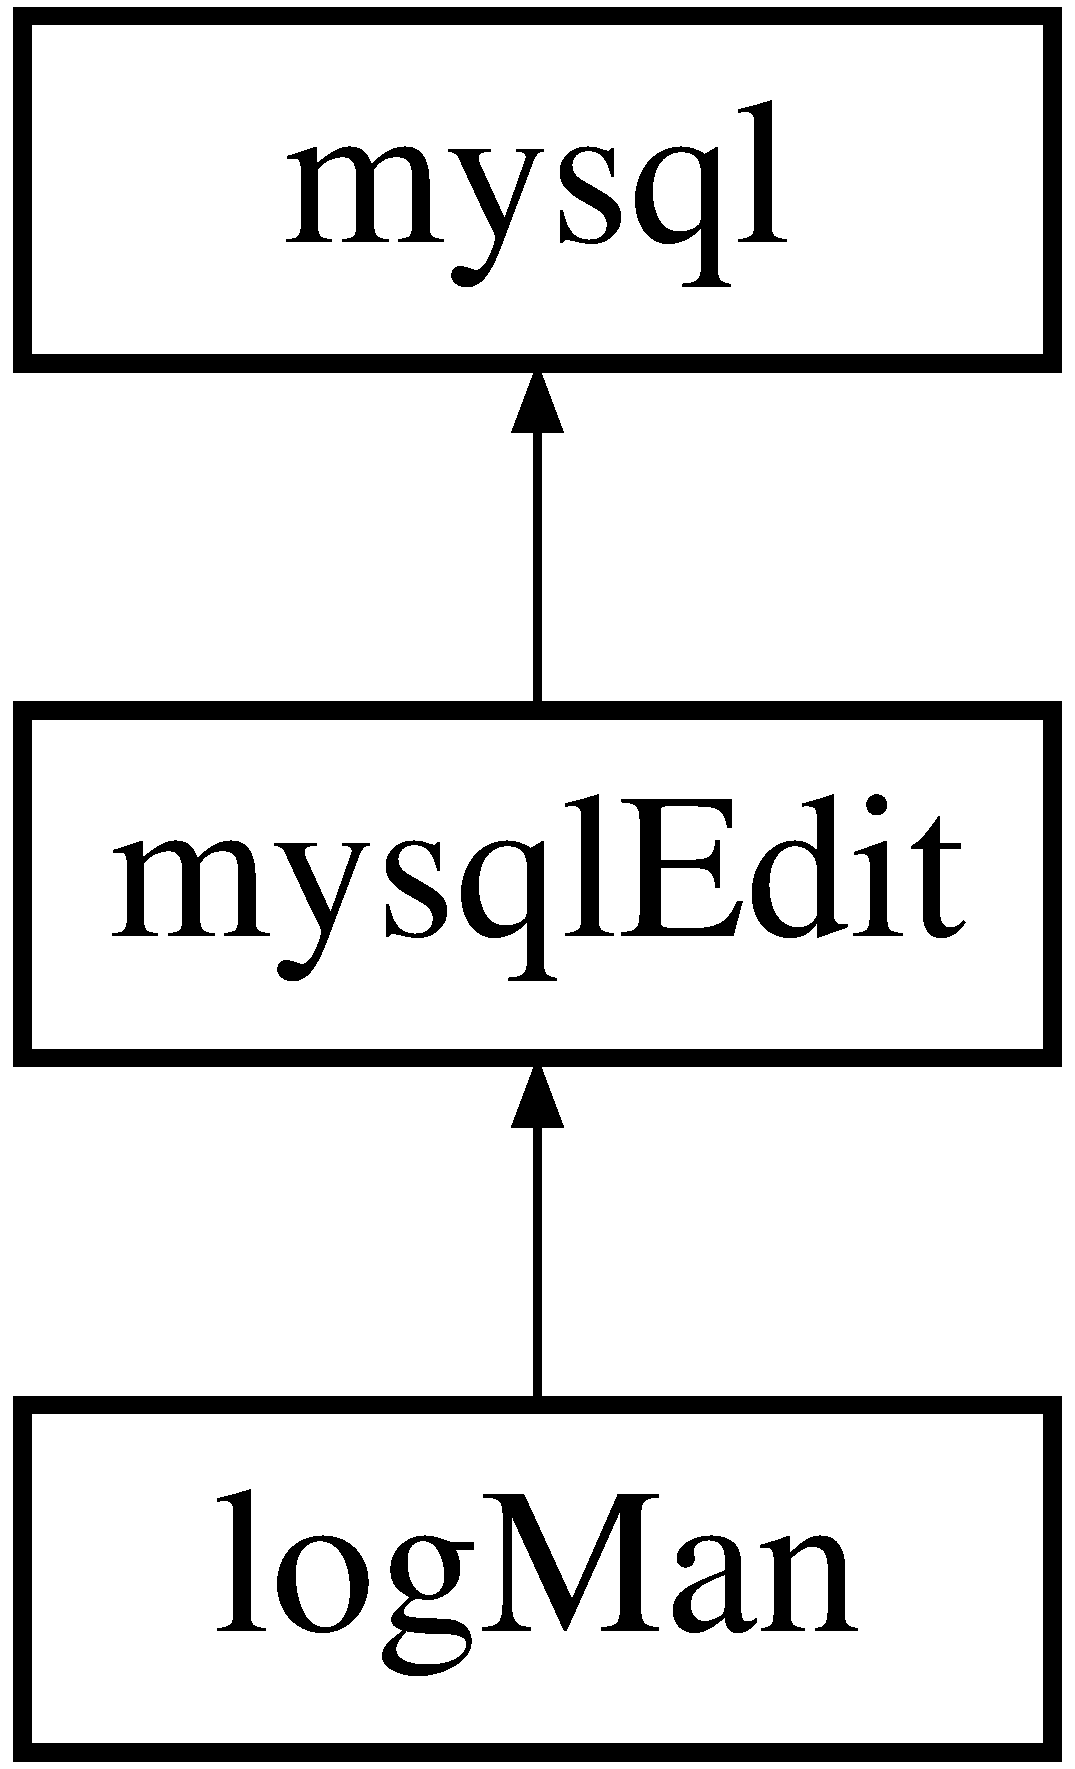
\includegraphics[height=3.000000cm]{classlog_man}
\end{center}
\end{figure}
\subsection*{Public Member Functions}
\begin{DoxyCompactItemize}
\item 
\hyperlink{classlog_man_aa966adc12c56a4cc70da92207fa50929}{install} ()
\item 
\hyperlink{classlog_man_a52a57cda7a4b849ed18d5c7133f75256}{edit\-Perm} (\$\hyperlink{classlog_man_a3b510811361c14194c4c54177f000f2d}{login}=null, \$perm=null)
\item 
\hyperlink{classlog_man_a3884708300d256bc4e2aed3d425ec00a}{get\-Perm} ()
\item 
\hyperlink{classlog_man_ae8162eecf899a411b0f91d013d16cda3}{create\-Super\-User} (\$email, \$name, \$pass)
\item 
\hyperlink{classlog_man_af787db5c087b93924fc5ac54e14775d5}{ereg} ()
\item 
\hyperlink{classlog_man_a3b510811361c14194c4c54177f000f2d}{login} (\$ajax)
\item 
\hyperlink{classlog_man_aa8dfc7c51361d8f550975be90ed2cf67}{check\-Session} (\$signal=false)
\item 
\hyperlink{classlog_man_a9a30d68c9f462839242a462ca43f5753}{basic\-Login} (\$\hyperlink{classtranslate}{translate}, \$seo)
\item 
\hyperlink{classlog_man_ab0912c8df7035bb6e9571a4333c0238a}{admin\-Login} (\$\hyperlink{classtranslate}{translate}, \$seo)
\item 
\hyperlink{classlog_man_a64ac0e06faad327b014754e951dfe170}{add\-To\-Main\-Array} (\$name, \$data)
\item 
\hyperlink{classlog_man_a89196d2fcfb896306fe7e387f634a080}{ajax\-Send\-Json} ()
\item 
\hypertarget{classlog_man_a7f3e615305910cf5ea9f24692e9613f6}{{\bfseries add\-New\-User} (\$pass, \$perm)}\label{classlog_man_a7f3e615305910cf5ea9f24692e9613f6}

\item 
\hyperlink{classlog_man_ad0c5594c7e33c9821afd4305edaee0b9}{create\-Session} ()
\item 
\hyperlink{classlog_man_a9aea96aaeaf1efd5531eb1867ee67ca6}{destroy\-Session} ()
\item 
\hyperlink{classlog_man_a63e86500ba57ad327c3cfdc4777b2edc}{add\-Session\-Data} (\$name, \$data=null)
\item 
\hyperlink{classlog_man_a0055230648d2a2484c489013a475c3d7}{get\-Session\-Data} (\$name)
\item 
\hypertarget{classlog_man_a0bb131a01e8d92cdecdc9013ca808013}{{\bfseries sign\-In} (\$pass)}\label{classlog_man_a0bb131a01e8d92cdecdc9013ca808013}

\item 
\hyperlink{classlog_man_ae99d103123f211eb28e19c09f7fd134e}{get\-Signed\-User} ()
\item 
\hypertarget{classlog_man_af6b7cbde6eae6ee4d7825b1a9f202bf6}{{\bfseries sign\-Out} ()}\label{classlog_man_af6b7cbde6eae6ee4d7825b1a9f202bf6}

\item 
\hyperlink{classlog_man_aff5b25c460fba7b1bce3e2a36fe702cf}{clean} (\$string)
\end{DoxyCompactItemize}
\subsection*{Protected Attributes}
\begin{DoxyCompactItemize}
\item 
\hypertarget{classlog_man_a9a2cf15a653aee8be437f7ae474cd494}{{\bfseries \$log} =array()}\label{classlog_man_a9a2cf15a653aee8be437f7ae474cd494}

\item 
\hypertarget{classlog_man_a58391ea75f2d29d5d708d7050b641c33}{{\bfseries \$status} =array()}\label{classlog_man_a58391ea75f2d29d5d708d7050b641c33}

\end{DoxyCompactItemize}
\subsection*{Additional Inherited Members}


\subsection{Detailed Description}


Definition at line 11 of file login.\-management.\-logman.\-php.



\subsection{Member Function Documentation}
\hypertarget{classlog_man_a63e86500ba57ad327c3cfdc4777b2edc}{\index{log\-Man@{log\-Man}!add\-Session\-Data@{add\-Session\-Data}}
\index{add\-Session\-Data@{add\-Session\-Data}!logMan@{log\-Man}}
\subsubsection[{add\-Session\-Data}]{\setlength{\rightskip}{0pt plus 5cm}add\-Session\-Data (
\begin{DoxyParamCaption}
\item[{}]{\$name, }
\item[{}]{\$data = {\ttfamily null}}
\end{DoxyParamCaption}
)\hspace{0.3cm}{\ttfamily [final]}}}\label{classlog_man_a63e86500ba57ad327c3cfdc4777b2edc}
Store data in new session 
\begin{DoxyParams}[1]{Parameters}
string & {\em \$name} & \\
\hline
string & {\em \$data} & \\
\hline
\end{DoxyParams}
\begin{DoxyReturn}{Returns}
string 
\end{DoxyReturn}


Definition at line 426 of file login.\-management.\-logman.\-php.

\hypertarget{classlog_man_a64ac0e06faad327b014754e951dfe170}{\index{log\-Man@{log\-Man}!add\-To\-Main\-Array@{add\-To\-Main\-Array}}
\index{add\-To\-Main\-Array@{add\-To\-Main\-Array}!logMan@{log\-Man}}
\subsubsection[{add\-To\-Main\-Array}]{\setlength{\rightskip}{0pt plus 5cm}add\-To\-Main\-Array (
\begin{DoxyParamCaption}
\item[{}]{\$name, }
\item[{}]{\$data}
\end{DoxyParamCaption}
)\hspace{0.3cm}{\ttfamily [final]}}}\label{classlog_man_a64ac0e06faad327b014754e951dfe170}
Add data to main login array 
\begin{DoxyParams}[1]{Parameters}
string & {\em \$name} & \\
\hline
multitype & {\em \$data} & \\
\hline
\end{DoxyParams}


Definition at line 379 of file login.\-management.\-logman.\-php.

\hypertarget{classlog_man_ab0912c8df7035bb6e9571a4333c0238a}{\index{log\-Man@{log\-Man}!admin\-Login@{admin\-Login}}
\index{admin\-Login@{admin\-Login}!logMan@{log\-Man}}
\subsubsection[{admin\-Login}]{\setlength{\rightskip}{0pt plus 5cm}admin\-Login (
\begin{DoxyParamCaption}
\item[{}]{\$translate, }
\item[{}]{\$seo}
\end{DoxyParamCaption}
)}}\label{classlog_man_ab0912c8df7035bb6e9571a4333c0238a}
Create default admin login system 
\begin{DoxyParams}[1]{Parameters}
object & {\em \$translate} & \\
\hline
object & {\em \$seo} & \\
\hline
\end{DoxyParams}
\begin{DoxyReturn}{Returns}
number 
\end{DoxyReturn}


Definition at line 335 of file login.\-management.\-logman.\-php.

\hypertarget{classlog_man_a89196d2fcfb896306fe7e387f634a080}{\index{log\-Man@{log\-Man}!ajax\-Send\-Json@{ajax\-Send\-Json}}
\index{ajax\-Send\-Json@{ajax\-Send\-Json}!logMan@{log\-Man}}
\subsubsection[{ajax\-Send\-Json}]{\setlength{\rightskip}{0pt plus 5cm}ajax\-Send\-Json (
\begin{DoxyParamCaption}
{}
\end{DoxyParamCaption}
)\hspace{0.3cm}{\ttfamily [final]}}}\label{classlog_man_a89196d2fcfb896306fe7e387f634a080}
Convert main array to J\-S\-O\-N export and print as A\-J\-A\-X response 

Definition at line 387 of file login.\-management.\-logman.\-php.

\hypertarget{classlog_man_a9a30d68c9f462839242a462ca43f5753}{\index{log\-Man@{log\-Man}!basic\-Login@{basic\-Login}}
\index{basic\-Login@{basic\-Login}!logMan@{log\-Man}}
\subsubsection[{basic\-Login}]{\setlength{\rightskip}{0pt plus 5cm}basic\-Login (
\begin{DoxyParamCaption}
\item[{}]{\$translate, }
\item[{}]{\$seo}
\end{DoxyParamCaption}
)}}\label{classlog_man_a9a30d68c9f462839242a462ca43f5753}
Create default login system 
\begin{DoxyParams}[1]{Parameters}
object & {\em \$translate} & \\
\hline
object & {\em \$seo} & \\
\hline
\end{DoxyParams}
\begin{DoxyReturn}{Returns}
number 
\end{DoxyReturn}


Definition at line 274 of file login.\-management.\-logman.\-php.

\hypertarget{classlog_man_aa8dfc7c51361d8f550975be90ed2cf67}{\index{log\-Man@{log\-Man}!check\-Session@{check\-Session}}
\index{check\-Session@{check\-Session}!logMan@{log\-Man}}
\subsubsection[{check\-Session}]{\setlength{\rightskip}{0pt plus 5cm}check\-Session (
\begin{DoxyParamCaption}
\item[{}]{\$signal = {\ttfamily false}}
\end{DoxyParamCaption}
)\hspace{0.3cm}{\ttfamily [final]}}}\label{classlog_man_aa8dfc7c51361d8f550975be90ed2cf67}
Check whether session


\begin{DoxyParams}[1]{Parameters}
bool & {\em \$signal} & \\
\hline
\end{DoxyParams}
\begin{DoxyReturn}{Returns}
boolean$\vert$\-Ambigous $<$multitype\-:number , multitype\-:$>$ 
\end{DoxyReturn}


Definition at line 252 of file login.\-management.\-logman.\-php.

\hypertarget{classlog_man_aff5b25c460fba7b1bce3e2a36fe702cf}{\index{log\-Man@{log\-Man}!clean@{clean}}
\index{clean@{clean}!logMan@{log\-Man}}
\subsubsection[{clean}]{\setlength{\rightskip}{0pt plus 5cm}clean (
\begin{DoxyParamCaption}
\item[{}]{\$string}
\end{DoxyParamCaption}
)\hspace{0.3cm}{\ttfamily [final]}}}\label{classlog_man_aff5b25c460fba7b1bce3e2a36fe702cf}
Remove all special characters 
\begin{DoxyParams}[1]{Parameters}
string & {\em \$string} & \\
\hline
\end{DoxyParams}
\begin{DoxyReturn}{Returns}
string 
\end{DoxyReturn}


Definition at line 467 of file login.\-management.\-logman.\-php.

\hypertarget{classlog_man_ad0c5594c7e33c9821afd4305edaee0b9}{\index{log\-Man@{log\-Man}!create\-Session@{create\-Session}}
\index{create\-Session@{create\-Session}!logMan@{log\-Man}}
\subsubsection[{create\-Session}]{\setlength{\rightskip}{0pt plus 5cm}create\-Session (
\begin{DoxyParamCaption}
{}
\end{DoxyParamCaption}
)\hspace{0.3cm}{\ttfamily [final]}}}\label{classlog_man_ad0c5594c7e33c9821afd4305edaee0b9}
Create session data \begin{DoxyReturn}{Returns}
multitype array 
\end{DoxyReturn}


Definition at line 401 of file login.\-management.\-logman.\-php.

\hypertarget{classlog_man_ae8162eecf899a411b0f91d013d16cda3}{\index{log\-Man@{log\-Man}!create\-Super\-User@{create\-Super\-User}}
\index{create\-Super\-User@{create\-Super\-User}!logMan@{log\-Man}}
\subsubsection[{create\-Super\-User}]{\setlength{\rightskip}{0pt plus 5cm}create\-Super\-User (
\begin{DoxyParamCaption}
\item[{}]{\$email, }
\item[{}]{\$name, }
\item[{}]{\$pass}
\end{DoxyParamCaption}
)\hspace{0.3cm}{\ttfamily [final]}}}\label{classlog_man_ae8162eecf899a411b0f91d013d16cda3}
Create admin user in database


\begin{DoxyParams}[1]{Parameters}
array & {\em \$\-\_\-\-P\-O\-S\-T} & \\
\hline
\end{DoxyParams}
\begin{DoxyReturn}{Returns}
array \$this-\/$>$status 
\end{DoxyReturn}


Definition at line 121 of file login.\-management.\-logman.\-php.

\hypertarget{classlog_man_a9aea96aaeaf1efd5531eb1867ee67ca6}{\index{log\-Man@{log\-Man}!destroy\-Session@{destroy\-Session}}
\index{destroy\-Session@{destroy\-Session}!logMan@{log\-Man}}
\subsubsection[{destroy\-Session}]{\setlength{\rightskip}{0pt plus 5cm}destroy\-Session (
\begin{DoxyParamCaption}
{}
\end{DoxyParamCaption}
)\hspace{0.3cm}{\ttfamily [final]}}}\label{classlog_man_a9aea96aaeaf1efd5531eb1867ee67ca6}
Destroy exist session 

Definition at line 413 of file login.\-management.\-logman.\-php.

\hypertarget{classlog_man_a52a57cda7a4b849ed18d5c7133f75256}{\index{log\-Man@{log\-Man}!edit\-Perm@{edit\-Perm}}
\index{edit\-Perm@{edit\-Perm}!logMan@{log\-Man}}
\subsubsection[{edit\-Perm}]{\setlength{\rightskip}{0pt plus 5cm}edit\-Perm (
\begin{DoxyParamCaption}
\item[{}]{\$login = {\ttfamily null}, }
\item[{}]{\$perm = {\ttfamily null}}
\end{DoxyParamCaption}
)\hspace{0.3cm}{\ttfamily [final]}}}\label{classlog_man_a52a57cda7a4b849ed18d5c7133f75256}
Update perm in \hyperlink{classlog_man}{log\-Man}


\begin{DoxyParams}{Parameters}
{\em string} & \\
\hline
{\em int} & (1000$\sim$1111)\\
\hline
\end{DoxyParams}
\begin{DoxyReturn}{Returns}
int O\-R false 
\end{DoxyReturn}


Definition at line 80 of file login.\-management.\-logman.\-php.

\hypertarget{classlog_man_af787db5c087b93924fc5ac54e14775d5}{\index{log\-Man@{log\-Man}!ereg@{ereg}}
\index{ereg@{ereg}!logMan@{log\-Man}}
\subsubsection[{ereg}]{\setlength{\rightskip}{0pt plus 5cm}ereg (
\begin{DoxyParamCaption}
{}
\end{DoxyParamCaption}
)\hspace{0.3cm}{\ttfamily [final]}}}\label{classlog_man_af787db5c087b93924fc5ac54e14775d5}
Create new user in database


\begin{DoxyParams}[1]{Parameters}
array & {\em \$\-\_\-\-P\-O\-S\-T} & \\
\hline
\end{DoxyParams}
\begin{DoxyReturn}{Returns}
array \$this-\/$>$status 
\end{DoxyReturn}


Definition at line 162 of file login.\-management.\-logman.\-php.

\hypertarget{classlog_man_a3884708300d256bc4e2aed3d425ec00a}{\index{log\-Man@{log\-Man}!get\-Perm@{get\-Perm}}
\index{get\-Perm@{get\-Perm}!logMan@{log\-Man}}
\subsubsection[{get\-Perm}]{\setlength{\rightskip}{0pt plus 5cm}get\-Perm (
\begin{DoxyParamCaption}
{}
\end{DoxyParamCaption}
)\hspace{0.3cm}{\ttfamily [final]}}}\label{classlog_man_a3884708300d256bc4e2aed3d425ec00a}
Returned actual user permission

\begin{DoxyReturn}{Returns}
int(4) 
\end{DoxyReturn}


Definition at line 109 of file login.\-management.\-logman.\-php.

\hypertarget{classlog_man_a0055230648d2a2484c489013a475c3d7}{\index{log\-Man@{log\-Man}!get\-Session\-Data@{get\-Session\-Data}}
\index{get\-Session\-Data@{get\-Session\-Data}!logMan@{log\-Man}}
\subsubsection[{get\-Session\-Data}]{\setlength{\rightskip}{0pt plus 5cm}get\-Session\-Data (
\begin{DoxyParamCaption}
\item[{}]{\$name}
\end{DoxyParamCaption}
)\hspace{0.3cm}{\ttfamily [final]}}}\label{classlog_man_a0055230648d2a2484c489013a475c3d7}
Get data from session storage 
\begin{DoxyParams}[1]{Parameters}
string & {\em \$name} & \\
\hline
\end{DoxyParams}
\begin{DoxyReturn}{Returns}
multitype 
\end{DoxyReturn}


Definition at line 437 of file login.\-management.\-logman.\-php.

\hypertarget{classlog_man_ae99d103123f211eb28e19c09f7fd134e}{\index{log\-Man@{log\-Man}!get\-Signed\-User@{get\-Signed\-User}}
\index{get\-Signed\-User@{get\-Signed\-User}!logMan@{log\-Man}}
\subsubsection[{get\-Signed\-User}]{\setlength{\rightskip}{0pt plus 5cm}get\-Signed\-User (
\begin{DoxyParamCaption}
{}
\end{DoxyParamCaption}
)\hspace{0.3cm}{\ttfamily [final]}}}\label{classlog_man_ae99d103123f211eb28e19c09f7fd134e}
Get all information about signed user

\begin{DoxyReturn}{Returns}
array 
\end{DoxyReturn}


Definition at line 452 of file login.\-management.\-logman.\-php.

\hypertarget{classlog_man_aa966adc12c56a4cc70da92207fa50929}{\index{log\-Man@{log\-Man}!install@{install}}
\index{install@{install}!logMan@{log\-Man}}
\subsubsection[{install}]{\setlength{\rightskip}{0pt plus 5cm}install (
\begin{DoxyParamCaption}
{}
\end{DoxyParamCaption}
)\hspace{0.3cm}{\ttfamily [final]}}}\label{classlog_man_aa966adc12c56a4cc70da92207fa50929}
Install \hyperlink{classlog_man}{log\-Man} if table not exist

\begin{DoxyReturn}{Returns}
bool 
\end{DoxyReturn}


Definition at line 43 of file login.\-management.\-logman.\-php.

\hypertarget{classlog_man_a3b510811361c14194c4c54177f000f2d}{\index{log\-Man@{log\-Man}!login@{login}}
\index{login@{login}!logMan@{log\-Man}}
\subsubsection[{login}]{\setlength{\rightskip}{0pt plus 5cm}login (
\begin{DoxyParamCaption}
\item[{}]{\$ajax}
\end{DoxyParamCaption}
)\hspace{0.3cm}{\ttfamily [final]}}}\label{classlog_man_a3b510811361c14194c4c54177f000f2d}
Login with ajax


\begin{DoxyParams}[1]{Parameters}
array & {\em \$ajax} & \\
\hline
\end{DoxyParams}
\begin{DoxyReturn}{Returns}
array \$this-\/$>$status 
\end{DoxyReturn}


Definition at line 203 of file login.\-management.\-logman.\-php.



The documentation for this class was generated from the following file\-:\begin{DoxyCompactItemize}
\item 
/home/peter/git/\-Open\-Sencillo/fw\-\_\-libraries/login.\-management.\-logman.\-php\end{DoxyCompactItemize}

\hypertarget{classmenu_gen}{\section{menu\-Gen Class Reference}
\label{classmenu_gen}\index{menu\-Gen@{menu\-Gen}}
}
\subsection*{Public Member Functions}
\begin{DoxyCompactItemize}
\item 
\hypertarget{classmenu_gen_ab2aa38e2757698073a9287059cf6cdba}{{\bfseries \-\_\-\-\_\-construct} (\$mysql\-Object, \$protocol, \$page, \$language, \$perm)}\label{classmenu_gen_ab2aa38e2757698073a9287059cf6cdba}

\item 
\hyperlink{classmenu_gen_ac188b81651695587a07ab3942871b244}{add\-Item\-To\-Menu} (\$c\-Base, \$c\-Sub\-Base, \$priority, \$perm, \$lang, \$c\-Name, \$c\-Href, \$c\-Title, \$c\-Image, \$c\-Image\-Alt)
\item 
\hyperlink{classmenu_gen_ad93ad5cfde55e9828416fe8e2fdb7b74}{create\-Menu} (\$name)
\item 
\hyperlink{classmenu_gen_a4009d0ea1a4ab80c3f19cb41bd457023}{switch\-Menu} (\$name)
\item 
\hypertarget{classmenu_gen_abebfe757962c5f97af6050764d680708}{{\bfseries generate\-Menu} (\$subcategory, \$level)}\label{classmenu_gen_abebfe757962c5f97af6050764d680708}

\item 
\hypertarget{classmenu_gen_a3c6b377051cfce54d0bc885ea61c7b7e}{{\bfseries generate\-Menu\-Level} (\$level, \$limit, \$page)}\label{classmenu_gen_a3c6b377051cfce54d0bc885ea61c7b7e}

\item 
\hyperlink{classmenu_gen_ae1715ef46ba484bce82b56ccd723c230}{generate\-Menu\-All\-Levels} (\$page)
\end{DoxyCompactItemize}
\subsection*{Data Fields}
\begin{DoxyCompactItemize}
\item 
\hypertarget{classmenu_gen_a3b6785d06028312e5e87edeb9363cdb1}{{\bfseries \$max\-Level} = array()}\label{classmenu_gen_a3b6785d06028312e5e87edeb9363cdb1}

\end{DoxyCompactItemize}
\subsection*{Protected Attributes}
\begin{DoxyCompactItemize}
\item 
\hypertarget{classmenu_gen_aec66dec69450671d861a4f23e8348b09}{{\bfseries \$mysql\-Object}}\label{classmenu_gen_aec66dec69450671d861a4f23e8348b09}

\item 
\hypertarget{classmenu_gen_ae858fe52917aca7da3e5f64ac5bf665a}{{\bfseries \$href}}\label{classmenu_gen_ae858fe52917aca7da3e5f64ac5bf665a}

\item 
\hypertarget{classmenu_gen_ab2fc40d43824ea3e1ce5d86dee0d763b}{{\bfseries \$name}}\label{classmenu_gen_ab2fc40d43824ea3e1ce5d86dee0d763b}

\item 
\hypertarget{classmenu_gen_ac01bf1cf041487498864d054b991f570}{{\bfseries \$protocol}}\label{classmenu_gen_ac01bf1cf041487498864d054b991f570}

\item 
\hypertarget{classmenu_gen_a0a44e6760141442bb439b1ab1395d8ff}{{\bfseries \$page}}\label{classmenu_gen_a0a44e6760141442bb439b1ab1395d8ff}

\item 
\hypertarget{classmenu_gen_a83170d318260a5a2e2a79dccdd371b10}{{\bfseries \$language}}\label{classmenu_gen_a83170d318260a5a2e2a79dccdd371b10}

\item 
\hypertarget{classmenu_gen_a680d99dc393b3de7d233c61670bef29c}{{\bfseries \$perm}}\label{classmenu_gen_a680d99dc393b3de7d233c61670bef29c}

\item 
\hypertarget{classmenu_gen_ac98296e470680a8cf4239e4acb58c545}{{\bfseries \$max\-Level\-Query}}\label{classmenu_gen_ac98296e470680a8cf4239e4acb58c545}

\end{DoxyCompactItemize}


\subsection{Detailed Description}


Definition at line 12 of file menu.\-generator.\-menugen.\-php.



\subsection{Member Function Documentation}
\hypertarget{classmenu_gen_ac188b81651695587a07ab3942871b244}{\index{menu\-Gen@{menu\-Gen}!add\-Item\-To\-Menu@{add\-Item\-To\-Menu}}
\index{add\-Item\-To\-Menu@{add\-Item\-To\-Menu}!menuGen@{menu\-Gen}}
\subsubsection[{add\-Item\-To\-Menu}]{\setlength{\rightskip}{0pt plus 5cm}add\-Item\-To\-Menu (
\begin{DoxyParamCaption}
\item[{}]{\$c\-Base, }
\item[{}]{\$c\-Sub\-Base, }
\item[{}]{\$priority, }
\item[{}]{\$perm, }
\item[{}]{\$lang, }
\item[{}]{\$c\-Name, }
\item[{}]{\$c\-Href, }
\item[{}]{\$c\-Title, }
\item[{}]{\$c\-Image, }
\item[{}]{\$c\-Image\-Alt}
\end{DoxyParamCaption}
)}}\label{classmenu_gen_ac188b81651695587a07ab3942871b244}
Add item to menu 
\begin{DoxyParams}{Parameters}
{\em int} & base \\
\hline
{\em int} & subbase \\
\hline
{\em int} & priority level \\
\hline
{\em int} & perm level \\
\hline
{\em int} & language id \\
\hline
{\em string} & name \\
\hline
{\em string} & href relative path as my/own/url \\
\hline
{\em string} & title text \\
\hline
{\em string} & image full path \\
\hline
{\em string} & image text alternative \\
\hline
\end{DoxyParams}


Definition at line 53 of file menu.\-generator.\-menugen.\-php.

\hypertarget{classmenu_gen_ad93ad5cfde55e9828416fe8e2fdb7b74}{\index{menu\-Gen@{menu\-Gen}!create\-Menu@{create\-Menu}}
\index{create\-Menu@{create\-Menu}!menuGen@{menu\-Gen}}
\subsubsection[{create\-Menu}]{\setlength{\rightskip}{0pt plus 5cm}create\-Menu (
\begin{DoxyParamCaption}
\item[{}]{\$name}
\end{DoxyParamCaption}
)}}\label{classmenu_gen_ad93ad5cfde55e9828416fe8e2fdb7b74}
Create menu structure and add new table to database 
\begin{DoxyParams}{Parameters}
{\em string} & table name \\
\hline
\end{DoxyParams}


Definition at line 78 of file menu.\-generator.\-menugen.\-php.

\hypertarget{classmenu_gen_ae1715ef46ba484bce82b56ccd723c230}{\index{menu\-Gen@{menu\-Gen}!generate\-Menu\-All\-Levels@{generate\-Menu\-All\-Levels}}
\index{generate\-Menu\-All\-Levels@{generate\-Menu\-All\-Levels}!menuGen@{menu\-Gen}}
\subsubsection[{generate\-Menu\-All\-Levels}]{\setlength{\rightskip}{0pt plus 5cm}generate\-Menu\-All\-Levels (
\begin{DoxyParamCaption}
\item[{}]{\$page}
\end{DoxyParamCaption}
)}}\label{classmenu_gen_ae1715ef46ba484bce82b56ccd723c230}
Generates show/hide menu levels 1-\/5  \$menu\-Gen-\/$>$generate\-Menu\-All\-Levels(\-P\-A\-G\-E);


\begin{DoxyParams}{Parameters}
{\em string} & \\
\hline
\end{DoxyParams}


Definition at line 631 of file menu.\-generator.\-menugen.\-php.

\hypertarget{classmenu_gen_a4009d0ea1a4ab80c3f19cb41bd457023}{\index{menu\-Gen@{menu\-Gen}!switch\-Menu@{switch\-Menu}}
\index{switch\-Menu@{switch\-Menu}!menuGen@{menu\-Gen}}
\subsubsection[{switch\-Menu}]{\setlength{\rightskip}{0pt plus 5cm}switch\-Menu (
\begin{DoxyParamCaption}
\item[{}]{\$name}
\end{DoxyParamCaption}
)}}\label{classmenu_gen_a4009d0ea1a4ab80c3f19cb41bd457023}
Switch menu by table name 
\begin{DoxyParams}{Parameters}
{\em string} & table name \\
\hline
\end{DoxyParams}


Definition at line 103 of file menu.\-generator.\-menugen.\-php.



The documentation for this class was generated from the following file\-:\begin{DoxyCompactItemize}
\item 
/home/peter/git/\-Open\-Sencillo/fw\-\_\-libraries/menu.\-generator.\-menugen.\-php\end{DoxyCompactItemize}

\hypertarget{classmysql}{\section{mysql Class Reference}
\label{classmysql}\index{mysql@{mysql}}
}
Inheritance diagram for mysql\-:\begin{figure}[H]
\begin{center}
\leavevmode
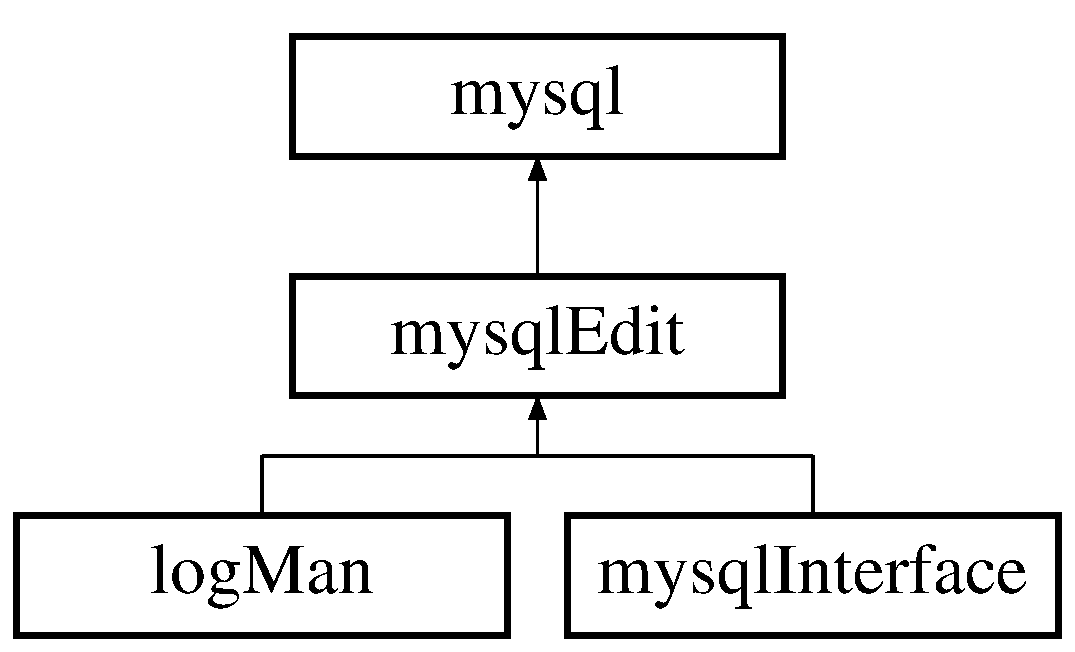
\includegraphics[height=3.000000cm]{classmysql}
\end{center}
\end{figure}
\subsection*{Public Member Functions}
\begin{DoxyCompactItemize}
\item 
\hyperlink{classmysql_a7af15455307c9b6a6c4d51d620014e7d}{\-\_\-\-\_\-construct} (\$D\-B\-Host=null, \$D\-B\-Name=null, \$D\-B\-User=null, \$D\-B\-Pass=null)
\item 
\hyperlink{classmysql_a6b251c8058230359b2922377699c4f29}{query} (\$sql)
\item 
\hyperlink{classmysql_a5c41f7192b0b3b866e15f56c431ddc36}{write} (\$sql)
\item 
\hyperlink{classmysql_aa69c8bf1f1dcf4e72552efff1fe3e87e}{close} ()
\item 
\hyperlink{classmysql_ad69dd4607977cae05ebe19d1ae604fb1}{test} ()
\item 
\hyperlink{classmysql_a2ddd43b5dd962bf0e23e9ce19e549ff3}{integrity} (\$type)
\end{DoxyCompactItemize}
\subsection*{Data Fields}
\begin{DoxyCompactItemize}
\item 
\hypertarget{classmysql_a1a881c28f710232dbf702d93c6a6e865}{{\bfseries \$\-D\-B\-Host}}\label{classmysql_a1a881c28f710232dbf702d93c6a6e865}

\item 
\hypertarget{classmysql_a3748d4d771a26c5411f1666a3a7a3cd8}{{\bfseries \$\-D\-B\-Name}}\label{classmysql_a3748d4d771a26c5411f1666a3a7a3cd8}

\item 
\hypertarget{classmysql_af107a7d38167b4ff8f65b395d856f7ab}{{\bfseries \$\-D\-B\-User}}\label{classmysql_af107a7d38167b4ff8f65b395d856f7ab}

\item 
\hypertarget{classmysql_a8cf3718595a762c1974c4adfa331bc58}{{\bfseries \$\-D\-B\-Pass}}\label{classmysql_a8cf3718595a762c1974c4adfa331bc58}

\item 
\hypertarget{classmysql_a0debe10448ec56a57b5509648408a549}{{\bfseries \$con}}\label{classmysql_a0debe10448ec56a57b5509648408a549}

\end{DoxyCompactItemize}


\subsection{Detailed Description}


Definition at line 11 of file core\-\_\-sql.\-php.



\subsection{Constructor \& Destructor Documentation}
\hypertarget{classmysql_a7af15455307c9b6a6c4d51d620014e7d}{\index{mysql@{mysql}!\-\_\-\-\_\-construct@{\-\_\-\-\_\-construct}}
\index{\-\_\-\-\_\-construct@{\-\_\-\-\_\-construct}!mysql@{mysql}}
\subsubsection[{\-\_\-\-\_\-construct}]{\setlength{\rightskip}{0pt plus 5cm}\-\_\-\-\_\-construct (
\begin{DoxyParamCaption}
\item[{}]{\$\-D\-B\-Host = {\ttfamily null}, }
\item[{}]{\$\-D\-B\-Name = {\ttfamily null}, }
\item[{}]{\$\-D\-B\-User = {\ttfamily null}, }
\item[{}]{\$\-D\-B\-Pass = {\ttfamily null}}
\end{DoxyParamCaption}
)}}\label{classmysql_a7af15455307c9b6a6c4d51d620014e7d}
Create connection 
\begin{DoxyParams}[1]{Parameters}
string & {\em \$\-D\-B\-Host} & \\
\hline
string & {\em \$\-D\-B\-Name} & \\
\hline
string & {\em \$\-D\-B\-User} & \\
\hline
string & {\em \$\-D\-B\-Pass} & \\
\hline
\end{DoxyParams}


Definition at line 27 of file core\-\_\-sql.\-php.



\subsection{Member Function Documentation}
\hypertarget{classmysql_aa69c8bf1f1dcf4e72552efff1fe3e87e}{\index{mysql@{mysql}!close@{close}}
\index{close@{close}!mysql@{mysql}}
\subsubsection[{close}]{\setlength{\rightskip}{0pt plus 5cm}close (
\begin{DoxyParamCaption}
{}
\end{DoxyParamCaption}
)\hspace{0.3cm}{\ttfamily [final]}}}\label{classmysql_aa69c8bf1f1dcf4e72552efff1fe3e87e}
Close database connection \begin{DoxyReturn}{Returns}
mixed 
\end{DoxyReturn}


Definition at line 73 of file core\-\_\-sql.\-php.

\hypertarget{classmysql_a2ddd43b5dd962bf0e23e9ce19e549ff3}{\index{mysql@{mysql}!integrity@{integrity}}
\index{integrity@{integrity}!mysql@{mysql}}
\subsubsection[{integrity}]{\setlength{\rightskip}{0pt plus 5cm}integrity (
\begin{DoxyParamCaption}
\item[{}]{\$type}
\end{DoxyParamCaption}
)\hspace{0.3cm}{\ttfamily [final]}}}\label{classmysql_a2ddd43b5dd962bf0e23e9ce19e549ff3}
Integrity check 
\begin{DoxyParams}{Parameters}
{\em string} & database type \\
\hline
\end{DoxyParams}


Definition at line 101 of file core\-\_\-sql.\-php.

\hypertarget{classmysql_a6b251c8058230359b2922377699c4f29}{\index{mysql@{mysql}!query@{query}}
\index{query@{query}!mysql@{mysql}}
\subsubsection[{query}]{\setlength{\rightskip}{0pt plus 5cm}query (
\begin{DoxyParamCaption}
\item[{}]{\$sql}
\end{DoxyParamCaption}
)\hspace{0.3cm}{\ttfamily [final]}}}\label{classmysql_a6b251c8058230359b2922377699c4f29}
Add query to database 
\begin{DoxyParams}[1]{Parameters}
string & {\em \$sql} & \\
\hline
\end{DoxyParams}
\begin{DoxyReturn}{Returns}
mixed resources 
\end{DoxyReturn}


Definition at line 54 of file core\-\_\-sql.\-php.

\hypertarget{classmysql_ad69dd4607977cae05ebe19d1ae604fb1}{\index{mysql@{mysql}!test@{test}}
\index{test@{test}!mysql@{mysql}}
\subsubsection[{test}]{\setlength{\rightskip}{0pt plus 5cm}test (
\begin{DoxyParamCaption}
{}
\end{DoxyParamCaption}
)\hspace{0.3cm}{\ttfamily [final]}}}\label{classmysql_ad69dd4607977cae05ebe19d1ae604fb1}
Test connection \begin{DoxyReturn}{Returns}
mixed 
\end{DoxyReturn}


Definition at line 82 of file core\-\_\-sql.\-php.

\hypertarget{classmysql_a5c41f7192b0b3b866e15f56c431ddc36}{\index{mysql@{mysql}!write@{write}}
\index{write@{write}!mysql@{mysql}}
\subsubsection[{write}]{\setlength{\rightskip}{0pt plus 5cm}write (
\begin{DoxyParamCaption}
\item[{}]{\$sql}
\end{DoxyParamCaption}
)\hspace{0.3cm}{\ttfamily [final]}}}\label{classmysql_a5c41f7192b0b3b866e15f56c431ddc36}
Add query to database 
\begin{DoxyParams}[1]{Parameters}
string & {\em \$sql} & \\
\hline
\end{DoxyParams}
\begin{DoxyReturn}{Returns}
mixed resources 
\end{DoxyReturn}


Definition at line 64 of file core\-\_\-sql.\-php.



The documentation for this class was generated from the following file\-:\begin{DoxyCompactItemize}
\item 
/home/peter/git/\-Open\-Sencillo/fw\-\_\-core/core\-\_\-sql.\-php\end{DoxyCompactItemize}

\hypertarget{classmysql_edit}{\section{mysql\-Edit Class Reference}
\label{classmysql_edit}\index{mysql\-Edit@{mysql\-Edit}}
}
Inheritance diagram for mysql\-Edit\-:\begin{figure}[H]
\begin{center}
\leavevmode
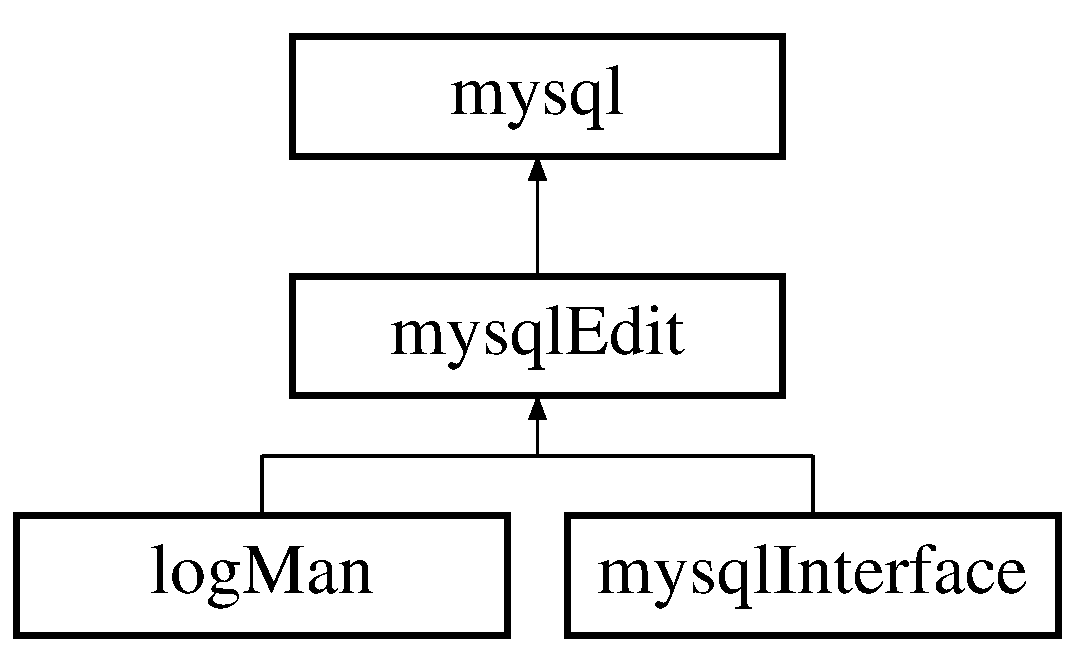
\includegraphics[height=3.000000cm]{classmysql_edit}
\end{center}
\end{figure}
\subsection*{Public Member Functions}
\begin{DoxyCompactItemize}
\item 
\hyperlink{classmysql_edit_afb4a6a8508ccd874c0ebd19ea9c6d7a3}{new\-Column} (\$name, \$type=\char`\"{}I\-N\-T\char`\"{})
\item 
\hyperlink{classmysql_edit_a20393378a29011bde0843665319c2ec7}{prepare\-Table} (\$name)
\item 
\hyperlink{classmysql_edit_af26ffcc175f4c1824af435ab0181fc47}{unique\-Key} (\$key\-Name)
\end{DoxyCompactItemize}
\begin{Indent}{\bf string \$name}\par
{\em Create table (use after new\-Column function) }\begin{DoxyCompactItemize}
\item 
\hypertarget{classmysql_edit_a1fb0787af4bf5891a0ac1ee919bcda1f}{{\bfseries create\-Table} (\$name)}\label{classmysql_edit_a1fb0787af4bf5891a0ac1ee919bcda1f}

\item 
\hyperlink{classmysql_edit_a46db6a2a866e7edcd9655e57343bda8a}{open\-Table} (\$name)
\item 
\hypertarget{classmysql_edit_ab76a899fa24ade276873e3bd1c34020c}{{\bfseries insert} (\$values)}\label{classmysql_edit_ab76a899fa24ade276873e3bd1c34020c}

\item 
\hyperlink{classmysql_edit_a9c81290e60bed5bcac4f233f8315a02d}{set} (\$column, \$value)
\item 
\hypertarget{classmysql_edit_ab2da7078237b1fc56a1621426df94391}{{\bfseries update} (\$if, \$sets=null)}\label{classmysql_edit_ab2da7078237b1fc56a1621426df94391}

\item 
\hypertarget{classmysql_edit_a54cfa86a296a1717ecdc7c667d8d238e}{{\bfseries delete} (\$if)}\label{classmysql_edit_a54cfa86a296a1717ecdc7c667d8d238e}

\item 
\hypertarget{classmysql_edit_a273362ae49e939816659e808d6b8aadc}{{\bfseries output} (\$if=\char`\"{}`id`$>$0\char`\"{}, \$order=\char`\"{}`id` A\-S\-C\char`\"{}, \$limit=1000)}\label{classmysql_edit_a273362ae49e939816659e808d6b8aadc}

\end{DoxyCompactItemize}
\end{Indent}
\subsection*{Additional Inherited Members}


\subsection{Detailed Description}


Definition at line 124 of file core\-\_\-sql.\-php.



\subsection{Member Function Documentation}
\hypertarget{classmysql_edit_afb4a6a8508ccd874c0ebd19ea9c6d7a3}{\index{mysql\-Edit@{mysql\-Edit}!new\-Column@{new\-Column}}
\index{new\-Column@{new\-Column}!mysqlEdit@{mysql\-Edit}}
\subsubsection[{new\-Column}]{\setlength{\rightskip}{0pt plus 5cm}new\-Column (
\begin{DoxyParamCaption}
\item[{}]{\$name, }
\item[{}]{\$type = {\ttfamily \char`\"{}INT\char`\"{}}}
\end{DoxyParamCaption}
)}}\label{classmysql_edit_afb4a6a8508ccd874c0ebd19ea9c6d7a3}
Create new column with type 
\begin{DoxyParams}[1]{Parameters}
string & {\em \$name} & column \\
\hline
string & {\em \$type} & column \\
\hline
\end{DoxyParams}


Definition at line 144 of file core\-\_\-sql.\-php.

\hypertarget{classmysql_edit_a46db6a2a866e7edcd9655e57343bda8a}{\index{mysql\-Edit@{mysql\-Edit}!open\-Table@{open\-Table}}
\index{open\-Table@{open\-Table}!mysqlEdit@{mysql\-Edit}}
\subsubsection[{open\-Table}]{\setlength{\rightskip}{0pt plus 5cm}open\-Table (
\begin{DoxyParamCaption}
\item[{}]{\$name}
\end{DoxyParamCaption}
)}}\label{classmysql_edit_a46db6a2a866e7edcd9655e57343bda8a}
Open table and read all column names 
\begin{DoxyParams}[1]{Parameters}
string & {\em \$name} & \\
\hline
\end{DoxyParams}


Definition at line 182 of file core\-\_\-sql.\-php.

\hypertarget{classmysql_edit_a20393378a29011bde0843665319c2ec7}{\index{mysql\-Edit@{mysql\-Edit}!prepare\-Table@{prepare\-Table}}
\index{prepare\-Table@{prepare\-Table}!mysqlEdit@{mysql\-Edit}}
\subsubsection[{prepare\-Table}]{\setlength{\rightskip}{0pt plus 5cm}prepare\-Table (
\begin{DoxyParamCaption}
\item[{}]{\$name}
\end{DoxyParamCaption}
)}}\label{classmysql_edit_a20393378a29011bde0843665319c2ec7}
Light alternative to open\-Table 
\begin{DoxyParams}[1]{Parameters}
string & {\em \$name} & \\
\hline
\end{DoxyParams}


Definition at line 153 of file core\-\_\-sql.\-php.

\hypertarget{classmysql_edit_a9c81290e60bed5bcac4f233f8315a02d}{\index{mysql\-Edit@{mysql\-Edit}!set@{set}}
\index{set@{set}!mysqlEdit@{mysql\-Edit}}
\subsubsection[{set}]{\setlength{\rightskip}{0pt plus 5cm}set (
\begin{DoxyParamCaption}
\item[{}]{\$column, }
\item[{}]{\$value}
\end{DoxyParamCaption}
)}}\label{classmysql_edit_a9c81290e60bed5bcac4f233f8315a02d}
Use befor update -\/ edit value in the column 
\begin{DoxyParams}[1]{Parameters}
string & {\em \$column} & \\
\hline
string & {\em \$value} & \\
\hline
\end{DoxyParams}


Definition at line 211 of file core\-\_\-sql.\-php.

\hypertarget{classmysql_edit_af26ffcc175f4c1824af435ab0181fc47}{\index{mysql\-Edit@{mysql\-Edit}!unique\-Key@{unique\-Key}}
\index{unique\-Key@{unique\-Key}!mysqlEdit@{mysql\-Edit}}
\subsubsection[{unique\-Key}]{\setlength{\rightskip}{0pt plus 5cm}unique\-Key (
\begin{DoxyParamCaption}
\item[{}]{\$key\-Name}
\end{DoxyParamCaption}
)}}\label{classmysql_edit_af26ffcc175f4c1824af435ab0181fc47}
Create unique key. Use after prepare\-Table. 
\begin{DoxyParams}[1]{Parameters}
string & {\em \$key\-Name} & \\
\hline
\end{DoxyParams}


Definition at line 162 of file core\-\_\-sql.\-php.



The documentation for this class was generated from the following file\-:\begin{DoxyCompactItemize}
\item 
/home/peter/git/\-Open\-Sencillo/fw\-\_\-core/core\-\_\-sql.\-php\end{DoxyCompactItemize}

\hypertarget{classmysql_interface}{\section{mysql\-Interface Class Reference}
\label{classmysql_interface}\index{mysql\-Interface@{mysql\-Interface}}
}
Inheritance diagram for mysql\-Interface\-:\begin{figure}[H]
\begin{center}
\leavevmode
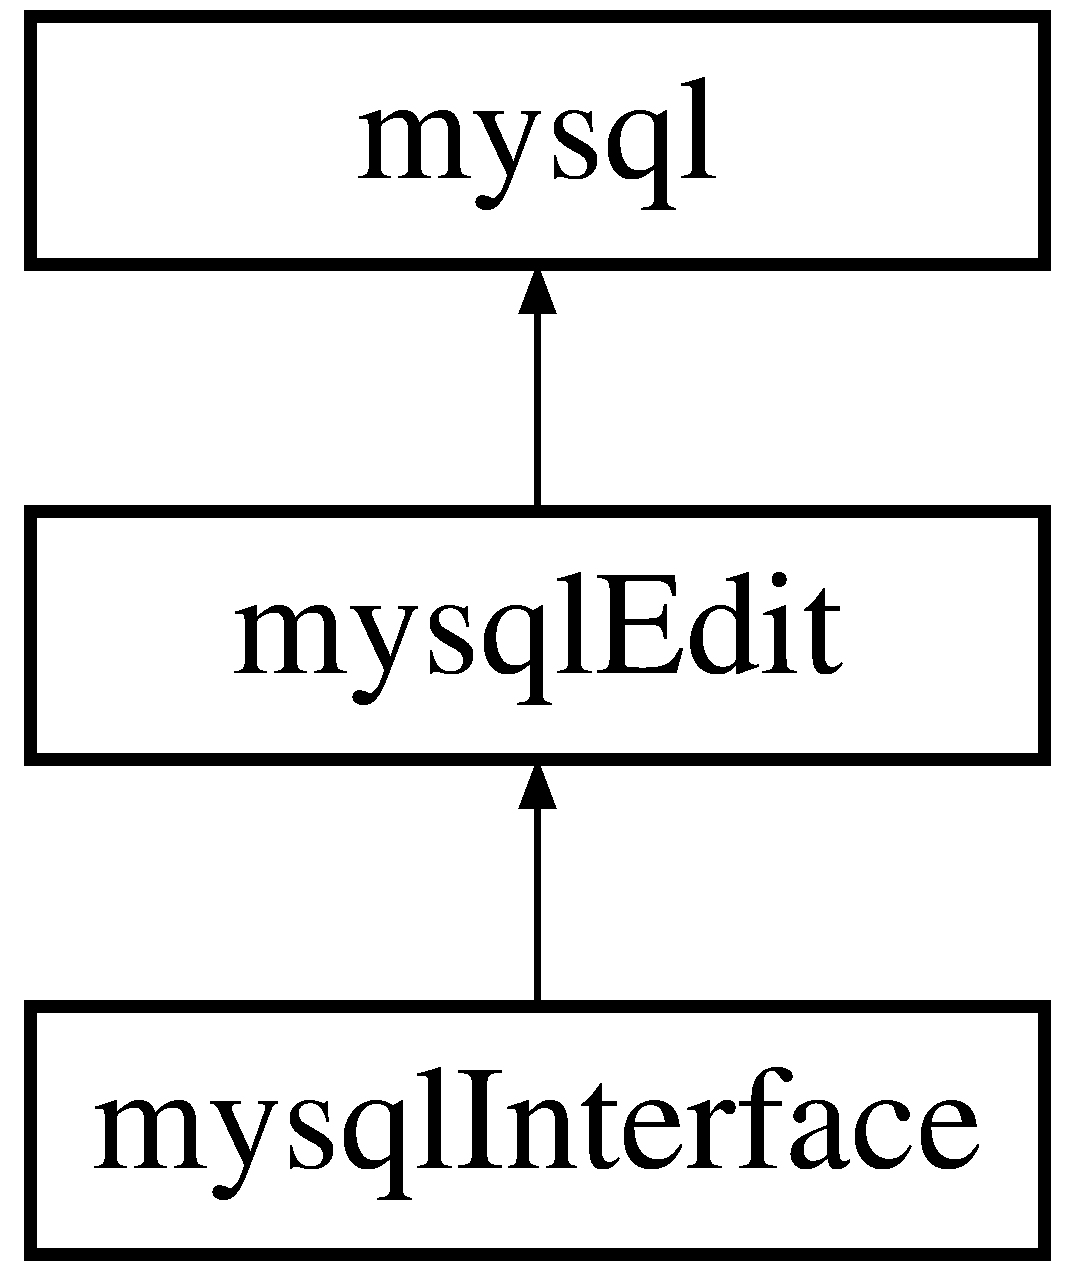
\includegraphics[height=3.000000cm]{classmysql_interface}
\end{center}
\end{figure}
\subsection*{Public Member Functions}
\begin{DoxyCompactItemize}
\item 
\hypertarget{classmysql_interface_ab8f860d15b6c8e90459cd3ee3a9a746b}{{\bfseries db\-Create\-Table} (\$array)}\label{classmysql_interface_ab8f860d15b6c8e90459cd3ee3a9a746b}

\item 
\hypertarget{classmysql_interface_a083e6cc172b111ec9c7eac0c9fae8a7a}{{\bfseries insert} (\$array, \$string\-Rewrite=true)}\label{classmysql_interface_a083e6cc172b111ec9c7eac0c9fae8a7a}

\item 
\hypertarget{classmysql_interface_a99e7e1b61e6e94996a4f9ddb84550a9c}{{\bfseries filter} (\$def)}\label{classmysql_interface_a99e7e1b61e6e94996a4f9ddb84550a9c}

\item 
\hypertarget{classmysql_interface_a3211e273c3ee674b966bab63d966c4b2}{{\bfseries update} (\$array)}\label{classmysql_interface_a3211e273c3ee674b966bab63d966c4b2}

\item 
\hyperlink{classmysql_interface_a1a124f363344d55e5d89910dca1b0ac5}{select} (\$array, \$update=false)
\item 
\hyperlink{classmysql_interface_a8a549a19ec81f3aafb2b231aaa12e138}{config} ()
\item 
\hyperlink{classmysql_interface_a78572828d11dcdf2a498497d9001d557}{connect} ()
\item 
\hyperlink{classmysql_interface_aba1c0c23ab9113d682823ea32a51332e}{validator} ()
\item 
\hyperlink{classmysql_interface_aaed74f7942d3fc56582e99324500e87b}{debug} ()
\item 
\hyperlink{classmysql_interface_a1909f4b7f8129c7790cb75de2ffbe1e4}{execute} ()
\end{DoxyCompactItemize}
\subsection*{Protected Attributes}
\begin{DoxyCompactItemize}
\item 
\hypertarget{classmysql_interface_a00e6dff44e00c36820da5508c6d9aba3}{{\bfseries \$save}}\label{classmysql_interface_a00e6dff44e00c36820da5508c6d9aba3}

\item 
\hypertarget{classmysql_interface_a580989e8e3521433691a0351287f6315}{{\bfseries \$mysqli}}\label{classmysql_interface_a580989e8e3521433691a0351287f6315}

\item 
\hypertarget{classmysql_interface_a956617395b85e98d907df712f6d0d3f7}{{\bfseries \$connect}}\label{classmysql_interface_a956617395b85e98d907df712f6d0d3f7}

\end{DoxyCompactItemize}
\subsection*{Additional Inherited Members}


\subsection{Detailed Description}
test need 

Definition at line 286 of file core\-\_\-sql.\-php.



\subsection{Member Function Documentation}
\hypertarget{classmysql_interface_a8a549a19ec81f3aafb2b231aaa12e138}{\index{mysql\-Interface@{mysql\-Interface}!config@{config}}
\index{config@{config}!mysqlInterface@{mysql\-Interface}}
\subsubsection[{config}]{\setlength{\rightskip}{0pt plus 5cm}config (
\begin{DoxyParamCaption}
{}
\end{DoxyParamCaption}
)}}\label{classmysql_interface_a8a549a19ec81f3aafb2b231aaa12e138}
Create database protected configuration arrray 

Definition at line 625 of file core\-\_\-sql.\-php.

\hypertarget{classmysql_interface_a78572828d11dcdf2a498497d9001d557}{\index{mysql\-Interface@{mysql\-Interface}!connect@{connect}}
\index{connect@{connect}!mysqlInterface@{mysql\-Interface}}
\subsubsection[{connect}]{\setlength{\rightskip}{0pt plus 5cm}connect (
\begin{DoxyParamCaption}
{}
\end{DoxyParamCaption}
)}}\label{classmysql_interface_a78572828d11dcdf2a498497d9001d557}
Create database connection 

Definition at line 650 of file core\-\_\-sql.\-php.

\hypertarget{classmysql_interface_aaed74f7942d3fc56582e99324500e87b}{\index{mysql\-Interface@{mysql\-Interface}!debug@{debug}}
\index{debug@{debug}!mysqlInterface@{mysql\-Interface}}
\subsubsection[{debug}]{\setlength{\rightskip}{0pt plus 5cm}debug (
\begin{DoxyParamCaption}
{}
\end{DoxyParamCaption}
)}}\label{classmysql_interface_aaed74f7942d3fc56582e99324500e87b}
Write query error log \begin{DoxySeeAlso}{See Also}
\hyperlink{classmysql_interface_aba1c0c23ab9113d682823ea32a51332e}{validator()} 
\end{DoxySeeAlso}
\begin{DoxyReturn}{Returns}
string 
\end{DoxyReturn}


Definition at line 692 of file core\-\_\-sql.\-php.

\hypertarget{classmysql_interface_a1909f4b7f8129c7790cb75de2ffbe1e4}{\index{mysql\-Interface@{mysql\-Interface}!execute@{execute}}
\index{execute@{execute}!mysqlInterface@{mysql\-Interface}}
\subsubsection[{execute}]{\setlength{\rightskip}{0pt plus 5cm}execute (
\begin{DoxyParamCaption}
{}
\end{DoxyParamCaption}
)}}\label{classmysql_interface_a1909f4b7f8129c7790cb75de2ffbe1e4}
Execute database multiline query and return result \begin{DoxyReturn}{Returns}
array\mbox{[}group\-\_\-id\mbox{]}\mbox{[}line\-\_\-id\mbox{]}\mbox{[}row\-\_\-name\mbox{]} 
\end{DoxyReturn}


Definition at line 701 of file core\-\_\-sql.\-php.

\hypertarget{classmysql_interface_a1a124f363344d55e5d89910dca1b0ac5}{\index{mysql\-Interface@{mysql\-Interface}!select@{select}}
\index{select@{select}!mysqlInterface@{mysql\-Interface}}
\subsubsection[{select}]{\setlength{\rightskip}{0pt plus 5cm}select (
\begin{DoxyParamCaption}
\item[{}]{\$array, }
\item[{}]{\$update = {\ttfamily false}}
\end{DoxyParamCaption}
)}}\label{classmysql_interface_a1a124f363344d55e5d89910dca1b0ac5}
ignore first N items

ignore last N items

out -\/ addcode

Definition at line 507 of file core\-\_\-sql.\-php.

\hypertarget{classmysql_interface_aba1c0c23ab9113d682823ea32a51332e}{\index{mysql\-Interface@{mysql\-Interface}!validator@{validator}}
\index{validator@{validator}!mysqlInterface@{mysql\-Interface}}
\subsubsection[{validator}]{\setlength{\rightskip}{0pt plus 5cm}validator (
\begin{DoxyParamCaption}
{}
\end{DoxyParamCaption}
)}}\label{classmysql_interface_aba1c0c23ab9113d682823ea32a51332e}
Check S\-Q\-L code for error \begin{DoxyReturn}{Returns}
bool 
\end{DoxyReturn}


Definition at line 675 of file core\-\_\-sql.\-php.



The documentation for this class was generated from the following file\-:\begin{DoxyCompactItemize}
\item 
/home/peter/git/\-Open\-Sencillo/fw\-\_\-core/core\-\_\-sql.\-php\end{DoxyCompactItemize}

\hypertarget{class_p_d_fto_j_p_g}{\section{P\-D\-Fto\-J\-P\-G Class Reference}
\label{class_p_d_fto_j_p_g}\index{P\-D\-Fto\-J\-P\-G@{P\-D\-Fto\-J\-P\-G}}
}
\subsection*{Public Member Functions}
\begin{DoxyCompactItemize}
\item 
\hyperlink{class_p_d_fto_j_p_g_ac4a417ed69f33e594ad12eceb846174c}{convert} (\$name, \$id=null, \$pdf\-Source=null, \$jpg\-Out\-Dir=null, \$quality=null)
\item 
\hyperlink{class_p_d_fto_j_p_g_aae3bfc864c34fb7c89abfbb0cbd5b296}{simulation} (\$name, \$id=null, \$pdf\-Source=null)
\item 
\hyperlink{class_p_d_fto_j_p_g_aa0a676d0c993727b170c6f7382d113d8}{pdf\-Path\-Generator} (\$name, \$id=null, \$pdf\-Source=null)
\item 
\hyperlink{class_p_d_fto_j_p_g_aa4659cafa5751c6ad17aabc467ad7958}{error\-List} ()
\item 
\hyperlink{class_p_d_fto_j_p_g_a33a69510fb3e90f4f6064ca10d47fc84}{in\-Path} (\$path)
\item 
\hyperlink{class_p_d_fto_j_p_g_a95fe4c5f4fb9d95bf52451a457870db9}{out\-Path} (\$path)
\end{DoxyCompactItemize}
\subsection*{Data Fields}
\begin{DoxyCompactItemize}
\item 
\hypertarget{class_p_d_fto_j_p_g_aeba2ab722cedda53dbb7ec1a59f45550}{{\bfseries \$error} =array()}\label{class_p_d_fto_j_p_g_aeba2ab722cedda53dbb7ec1a59f45550}

\item 
\hypertarget{class_p_d_fto_j_p_g_a0a4baf0b22973c07685c3981f0d17fc4}{{\bfseries \$path} =array()}\label{class_p_d_fto_j_p_g_a0a4baf0b22973c07685c3981f0d17fc4}

\end{DoxyCompactItemize}


\subsection{Detailed Description}


Definition at line 11 of file imagick.\-convert.\-pdf2jpg.\-php.



\subsection{Member Function Documentation}
\hypertarget{class_p_d_fto_j_p_g_ac4a417ed69f33e594ad12eceb846174c}{\index{P\-D\-Fto\-J\-P\-G@{P\-D\-Fto\-J\-P\-G}!convert@{convert}}
\index{convert@{convert}!PDFtoJPG@{P\-D\-Fto\-J\-P\-G}}
\subsubsection[{convert}]{\setlength{\rightskip}{0pt plus 5cm}convert (
\begin{DoxyParamCaption}
\item[{}]{\$name, }
\item[{}]{\$id = {\ttfamily null}, }
\item[{}]{\$pdf\-Source = {\ttfamily null}, }
\item[{}]{\$jpg\-Out\-Dir = {\ttfamily null}, }
\item[{}]{\$quality = {\ttfamily null}}
\end{DoxyParamCaption}
)}}\label{class_p_d_fto_j_p_g_ac4a417ed69f33e594ad12eceb846174c}
Convert P\-D\-F to J\-P\-G via P\-H\-P imagick


\begin{DoxyParams}[1]{Parameters}
string & {\em \$name} & (name input file) \\
\hline
number & {\em \$id} & (numeric user id if system using id) \\
\hline
string & {\em \$pdf\-Source} & (pdf source path) \\
\hline
string & {\em \$jpg\-Out\-Dir} & (jpg out root dir path)\\
\hline
\end{DoxyParams}
\begin{DoxyReturn}{Returns}
number 
\end{DoxyReturn}


Definition at line 27 of file imagick.\-convert.\-pdf2jpg.\-php.

\hypertarget{class_p_d_fto_j_p_g_aa4659cafa5751c6ad17aabc467ad7958}{\index{P\-D\-Fto\-J\-P\-G@{P\-D\-Fto\-J\-P\-G}!error\-List@{error\-List}}
\index{error\-List@{error\-List}!PDFtoJPG@{P\-D\-Fto\-J\-P\-G}}
\subsubsection[{error\-List}]{\setlength{\rightskip}{0pt plus 5cm}error\-List (
\begin{DoxyParamCaption}
{}
\end{DoxyParamCaption}
)}}\label{class_p_d_fto_j_p_g_aa4659cafa5751c6ad17aabc467ad7958}
Get last error 

Definition at line 132 of file imagick.\-convert.\-pdf2jpg.\-php.

\hypertarget{class_p_d_fto_j_p_g_a33a69510fb3e90f4f6064ca10d47fc84}{\index{P\-D\-Fto\-J\-P\-G@{P\-D\-Fto\-J\-P\-G}!in\-Path@{in\-Path}}
\index{in\-Path@{in\-Path}!PDFtoJPG@{P\-D\-Fto\-J\-P\-G}}
\subsubsection[{in\-Path}]{\setlength{\rightskip}{0pt plus 5cm}in\-Path (
\begin{DoxyParamCaption}
\item[{}]{\$path}
\end{DoxyParamCaption}
)}}\label{class_p_d_fto_j_p_g_a33a69510fb3e90f4f6064ca10d47fc84}
Path finder for testing 
\begin{DoxyParams}{Parameters}
{\em string} & \\
\hline
\end{DoxyParams}


Definition at line 141 of file imagick.\-convert.\-pdf2jpg.\-php.

\hypertarget{class_p_d_fto_j_p_g_a95fe4c5f4fb9d95bf52451a457870db9}{\index{P\-D\-Fto\-J\-P\-G@{P\-D\-Fto\-J\-P\-G}!out\-Path@{out\-Path}}
\index{out\-Path@{out\-Path}!PDFtoJPG@{P\-D\-Fto\-J\-P\-G}}
\subsubsection[{out\-Path}]{\setlength{\rightskip}{0pt plus 5cm}out\-Path (
\begin{DoxyParamCaption}
\item[{}]{\$path}
\end{DoxyParamCaption}
)}}\label{class_p_d_fto_j_p_g_a95fe4c5f4fb9d95bf52451a457870db9}
Path finder for testing 
\begin{DoxyParams}{Parameters}
{\em string} & \\
\hline
\end{DoxyParams}


Definition at line 151 of file imagick.\-convert.\-pdf2jpg.\-php.

\hypertarget{class_p_d_fto_j_p_g_aa0a676d0c993727b170c6f7382d113d8}{\index{P\-D\-Fto\-J\-P\-G@{P\-D\-Fto\-J\-P\-G}!pdf\-Path\-Generator@{pdf\-Path\-Generator}}
\index{pdf\-Path\-Generator@{pdf\-Path\-Generator}!PDFtoJPG@{P\-D\-Fto\-J\-P\-G}}
\subsubsection[{pdf\-Path\-Generator}]{\setlength{\rightskip}{0pt plus 5cm}pdf\-Path\-Generator (
\begin{DoxyParamCaption}
\item[{}]{\$name, }
\item[{}]{\$id = {\ttfamily null}, }
\item[{}]{\$pdf\-Source = {\ttfamily null}}
\end{DoxyParamCaption}
)}}\label{class_p_d_fto_j_p_g_aa0a676d0c993727b170c6f7382d113d8}
Convert simulation for generate path to source. Without Image\-Magic php extension.


\begin{DoxyParams}[1]{Parameters}
string & {\em \$name} & (name input file) \\
\hline
number & {\em \$id} & (numeric user id if system using id) \\
\hline
string & {\em \$pdf\-Source} & (pdf source path)\\
\hline
\end{DoxyParams}
\begin{DoxyReturn}{Returns}
mixed 
\end{DoxyReturn}


Definition at line 120 of file imagick.\-convert.\-pdf2jpg.\-php.

\hypertarget{class_p_d_fto_j_p_g_aae3bfc864c34fb7c89abfbb0cbd5b296}{\index{P\-D\-Fto\-J\-P\-G@{P\-D\-Fto\-J\-P\-G}!simulation@{simulation}}
\index{simulation@{simulation}!PDFtoJPG@{P\-D\-Fto\-J\-P\-G}}
\subsubsection[{simulation}]{\setlength{\rightskip}{0pt plus 5cm}simulation (
\begin{DoxyParamCaption}
\item[{}]{\$name, }
\item[{}]{\$id = {\ttfamily null}, }
\item[{}]{\$pdf\-Source = {\ttfamily null}}
\end{DoxyParamCaption}
)}}\label{class_p_d_fto_j_p_g_aae3bfc864c34fb7c89abfbb0cbd5b296}
Convert simulation


\begin{DoxyParams}[1]{Parameters}
string & {\em \$name} & (name input file) \\
\hline
number & {\em \$id} & (numeric user id if system using id) \\
\hline
string & {\em \$pdf\-Source} & (pdf source path)\\
\hline
\end{DoxyParams}
\begin{DoxyReturn}{Returns}
mixed 
\end{DoxyReturn}


Definition at line 83 of file imagick.\-convert.\-pdf2jpg.\-php.



The documentation for this class was generated from the following file\-:\begin{DoxyCompactItemize}
\item 
/home/peter/git/\-Open\-Sencillo/fw\-\_\-libraries/imagick.\-convert.\-pdf2jpg.\-php\end{DoxyCompactItemize}

\hypertarget{classsession_manager}{\section{session\-Manager Class Reference}
\label{classsession_manager}\index{session\-Manager@{session\-Manager}}
}
Inheritance diagram for session\-Manager\-:\begin{figure}[H]
\begin{center}
\leavevmode
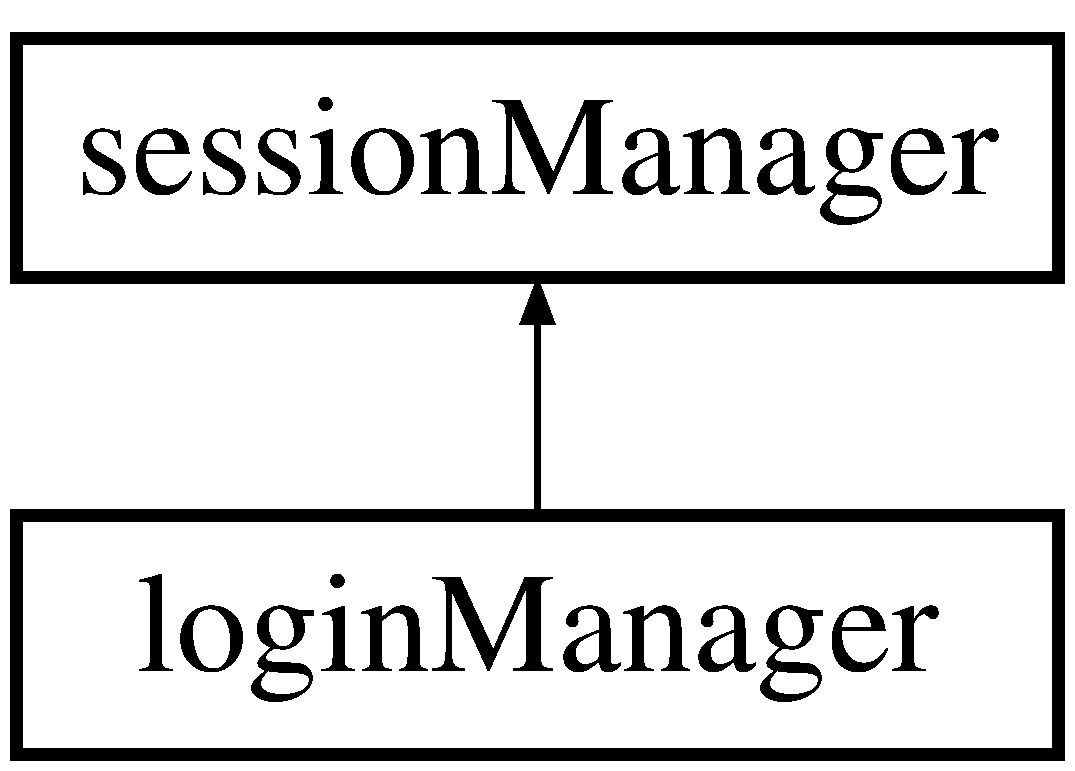
\includegraphics[height=2.000000cm]{classsession_manager}
\end{center}
\end{figure}
\subsection*{Public Member Functions}
\begin{DoxyCompactItemize}
\item 
\hyperlink{classsession_manager_a095c5d389db211932136b53f25f39685}{\-\_\-\-\_\-construct} ()
\item 
\hyperlink{classsession_manager_aa0196c5f4e75779c2067d9e4a03336d1}{sm\-\_\-get} (\$name)
\item 
\hyperlink{classsession_manager_a5aa4f941ff83651a35bb1f30afe415f9}{sm\-\_\-destroy} ()
\end{DoxyCompactItemize}


\subsection{Detailed Description}


Definition at line 27 of file session.\-php.



\subsection{Constructor \& Destructor Documentation}
\hypertarget{classsession_manager_a095c5d389db211932136b53f25f39685}{\index{session\-Manager@{session\-Manager}!\-\_\-\-\_\-construct@{\-\_\-\-\_\-construct}}
\index{\-\_\-\-\_\-construct@{\-\_\-\-\_\-construct}!sessionManager@{session\-Manager}}
\subsubsection[{\-\_\-\-\_\-construct}]{\setlength{\rightskip}{0pt plus 5cm}\-\_\-\-\_\-construct (
\begin{DoxyParamCaption}
{}
\end{DoxyParamCaption}
)}}\label{classsession_manager_a095c5d389db211932136b53f25f39685}
Create new session or reload old session 

Definition at line 35 of file session.\-php.



\subsection{Member Function Documentation}
\hypertarget{classsession_manager_a5aa4f941ff83651a35bb1f30afe415f9}{\index{session\-Manager@{session\-Manager}!sm\-\_\-destroy@{sm\-\_\-destroy}}
\index{sm\-\_\-destroy@{sm\-\_\-destroy}!sessionManager@{session\-Manager}}
\subsubsection[{sm\-\_\-destroy}]{\setlength{\rightskip}{0pt plus 5cm}sm\-\_\-destroy (
\begin{DoxyParamCaption}
{}
\end{DoxyParamCaption}
)}}\label{classsession_manager_a5aa4f941ff83651a35bb1f30afe415f9}
Session destroy 

Definition at line 66 of file session.\-php.

\hypertarget{classsession_manager_aa0196c5f4e75779c2067d9e4a03336d1}{\index{session\-Manager@{session\-Manager}!sm\-\_\-get@{sm\-\_\-get}}
\index{sm\-\_\-get@{sm\-\_\-get}!sessionManager@{session\-Manager}}
\subsubsection[{sm\-\_\-get}]{\setlength{\rightskip}{0pt plus 5cm}sm\-\_\-get (
\begin{DoxyParamCaption}
\item[{}]{\$name}
\end{DoxyParamCaption}
)}}\label{classsession_manager_aa0196c5f4e75779c2067d9e4a03336d1}
Get stored data from session 
\begin{DoxyParams}[1]{Parameters}
string & {\em \$name} & \\
\hline
\end{DoxyParams}
\begin{DoxyReturn}{Returns}
mixed 
\end{DoxyReturn}


Definition at line 45 of file session.\-php.



The documentation for this class was generated from the following file\-:\begin{DoxyCompactItemize}
\item 
/home/peter/git/\-Open\-Sencillo/fw\-\_\-headers/session.\-php\end{DoxyCompactItemize}

\hypertarget{classabeautifulsite_1_1_simple_image}{\section{Simple\-Image Class Reference}
\label{classabeautifulsite_1_1_simple_image}\index{Simple\-Image@{Simple\-Image}}
}
\subsection*{Public Member Functions}
\begin{DoxyCompactItemize}
\item 
\hyperlink{classabeautifulsite_1_1_simple_image_ae69773d7ae7457ff1524174317f6ad62}{\-\_\-\-\_\-construct} (\$filename=null, \$width=null, \$height=null, \$color=null)
\item 
\hyperlink{classabeautifulsite_1_1_simple_image_a421831a265621325e1fdd19aace0c758}{\-\_\-\-\_\-destruct} ()
\item 
\hyperlink{classabeautifulsite_1_1_simple_image_a1e67e72870ddf87f3d16b3010cd7d3f2}{adaptive\-\_\-resize} (\$width, \$height=null)
\item 
\hyperlink{classabeautifulsite_1_1_simple_image_a0ed80eb3d0f683447f8c163aba89cc84}{auto\-\_\-orient} ()
\item 
\hyperlink{classabeautifulsite_1_1_simple_image_aaced3f2b7cc91ab8891d9248139338cf}{best\-\_\-fit} (\$max\-\_\-width, \$max\-\_\-height)
\item 
\hyperlink{classabeautifulsite_1_1_simple_image_a693a4a7bc49924eb8c7ca586c3fbc2ba}{blur} (\$type= 'selective', \$passes=1)
\item 
\hyperlink{classabeautifulsite_1_1_simple_image_af571c7cddbd8021822dc8a6c36bd4059}{brightness} (\$level)
\item 
\hyperlink{classabeautifulsite_1_1_simple_image_a7af23605eb273c1084cbbf092bf69c50}{contrast} (\$level)
\item 
\hyperlink{classabeautifulsite_1_1_simple_image_ab133aa5541f0ae97c49d5729ace52c62}{colorize} (\$color, \$\hyperlink{classabeautifulsite_1_1_simple_image_add5b914f35ec96d98f9e3026693a627d}{opacity})
\item 
\hyperlink{classabeautifulsite_1_1_simple_image_aae0bbd9a1af614db7c62fcfcdb906ecb}{create} (\$width, \$height=null, \$color=null)
\item 
\hyperlink{classabeautifulsite_1_1_simple_image_a4363bcc58d31e100cc126fafad73ef1a}{crop} (\$x1, \$y1, \$x2, \$y2)
\item 
\hyperlink{classabeautifulsite_1_1_simple_image_aac9e0740c42741b5b9f2e61991a34112}{desaturate} ()
\item 
\hyperlink{classabeautifulsite_1_1_simple_image_aed0804dc7416329172ab55bcbf1d41b7}{edges} ()
\item 
\hyperlink{classabeautifulsite_1_1_simple_image_aabc8c1473621bfe3e064dd0a756c935e}{emboss} ()
\item 
\hyperlink{classabeautifulsite_1_1_simple_image_aaa59492eca3655d941d74c92eff212e9}{fill} (\$color= '\#000000')
\item 
\hyperlink{classabeautifulsite_1_1_simple_image_a8336e743a25f5301892696cd7c394f1f}{fit\-\_\-to\-\_\-height} (\$height)
\item 
\hyperlink{classabeautifulsite_1_1_simple_image_ac94ed3e74548edbf50883dc09790ab16}{fit\-\_\-to\-\_\-width} (\$width)
\item 
\hyperlink{classabeautifulsite_1_1_simple_image_afbed21df0630ae4d62c6ba38edd6f9d1}{flip} (\$direction)
\item 
\hyperlink{classabeautifulsite_1_1_simple_image_a0acd49b80218568ea04e7a5886373c54}{get\-\_\-height} ()
\item 
\hyperlink{classabeautifulsite_1_1_simple_image_a6bb3cbd0b8cb4156b2521365fca79529}{get\-\_\-orientation} ()
\item 
\hyperlink{classabeautifulsite_1_1_simple_image_a2514a0242e2b19b8b5fcbd7a79db5527}{get\-\_\-original\-\_\-info} ()
\item 
\hyperlink{classabeautifulsite_1_1_simple_image_abb10ccd258503d273acaf265bf1b1535}{get\-\_\-width} ()
\item 
\hyperlink{classabeautifulsite_1_1_simple_image_a70a743c63f97d5bbfdb2cdab7d186938}{invert} ()
\item 
\hyperlink{classabeautifulsite_1_1_simple_image_a585c262d16bad21a05af8804df8372b2}{load} (\$filename)
\item 
\hyperlink{classabeautifulsite_1_1_simple_image_a21c21cee2c0a9cd9e8965a684f50e8e8}{load\-\_\-base64} (\$base64string)
\item 
\hyperlink{classabeautifulsite_1_1_simple_image_a4f2623f77a0eb2993c39668604b9d028}{mean\-\_\-remove} ()
\item 
\hyperlink{classabeautifulsite_1_1_simple_image_add5b914f35ec96d98f9e3026693a627d}{opacity} (\$opacity)
\item 
\hyperlink{classabeautifulsite_1_1_simple_image_a1d8a0c4ee571db448e556caed12028d1}{output} (\$format=null, \$quality=null)
\item 
\hyperlink{classabeautifulsite_1_1_simple_image_acd08ab8d9a2213db91dc8a4cd533fedc}{output\-\_\-base64} (\$format=null, \$quality=null)
\item 
\hyperlink{classabeautifulsite_1_1_simple_image_ab2dbc20c617a63e98ab1249031a4f65a}{overlay} (\$overlay, \$position= 'center', \$\hyperlink{classabeautifulsite_1_1_simple_image_add5b914f35ec96d98f9e3026693a627d}{opacity}=1, \$x\-\_\-offset=0, \$y\-\_\-offset=0)
\item 
\hyperlink{classabeautifulsite_1_1_simple_image_a682af070180fbd1f3734653757403139}{pixelate} (\$block\-\_\-size=10)
\item 
\hyperlink{classabeautifulsite_1_1_simple_image_aa22cf38c82a9f8234d99293ada1f70fa}{resize} (\$width, \$height)
\item 
\hyperlink{classabeautifulsite_1_1_simple_image_a2c6d126f21bff5223d7d7f9bdb54cf79}{rotate} (\$angle, \$bg\-\_\-color= '\#000000')
\item 
\hyperlink{classabeautifulsite_1_1_simple_image_a23cd0d0e54d1453a48d8d21ff9f65ae6}{save} (\$filename=null, \$quality=null)
\item 
\hyperlink{classabeautifulsite_1_1_simple_image_a4723159606519b101e408854bc65ee35}{sepia} ()
\item 
\hyperlink{classabeautifulsite_1_1_simple_image_afc92209cb2a19193d46a9338b13a3bb9}{sketch} ()
\item 
\hyperlink{classabeautifulsite_1_1_simple_image_a7ebc6366f3da2bf2af1608663fdb7a09}{smooth} (\$level)
\item 
\hyperlink{classabeautifulsite_1_1_simple_image_a7dff268d38b2b142b38c7a495bc439c0}{text} (\$text, \$font\-\_\-file, \$font\-\_\-size=12, \$color= '\#000000', \$position= 'center', \$x\-\_\-offset=0, \$y\-\_\-offset=0)
\item 
\hyperlink{classabeautifulsite_1_1_simple_image_a48003368138dcf4baf3e06f5e5599b8d}{thumbnail} (\$width, \$height=null)
\end{DoxyCompactItemize}
\subsection*{Data Fields}
\begin{DoxyCompactItemize}
\item 
\hypertarget{classabeautifulsite_1_1_simple_image_a0e342ea32cccdc2c932ad23b9796a62a}{{\bfseries \$quality} = 80}\label{classabeautifulsite_1_1_simple_image_a0e342ea32cccdc2c932ad23b9796a62a}

\item 
\hypertarget{classabeautifulsite_1_1_simple_image_a0722441477f957078ee2437054556cbc}{{\bfseries \$filename}}\label{classabeautifulsite_1_1_simple_image_a0722441477f957078ee2437054556cbc}

\item 
\hypertarget{classabeautifulsite_1_1_simple_image_ab0f3ea69c9d9d311d11940fe4784a353}{{\bfseries \$original\-\_\-info}}\label{classabeautifulsite_1_1_simple_image_ab0f3ea69c9d9d311d11940fe4784a353}

\item 
\hypertarget{classabeautifulsite_1_1_simple_image_a5795120b4b324bc4ca83f1e6fdce7d57}{{\bfseries \$width}}\label{classabeautifulsite_1_1_simple_image_a5795120b4b324bc4ca83f1e6fdce7d57}

\item 
\hypertarget{classabeautifulsite_1_1_simple_image_a2c265bba1724371bb03e6901297c30b2}{{\bfseries \$height}}\label{classabeautifulsite_1_1_simple_image_a2c265bba1724371bb03e6901297c30b2}

\item 
\hypertarget{classabeautifulsite_1_1_simple_image_a3abffbc75cede9a7ba56156c8dec06c0}{{\bfseries \$imagestring}}\label{classabeautifulsite_1_1_simple_image_a3abffbc75cede9a7ba56156c8dec06c0}

\end{DoxyCompactItemize}
\subsection*{Protected Member Functions}
\begin{DoxyCompactItemize}
\item 
\hyperlink{classabeautifulsite_1_1_simple_image_ae0e4ad34b7a0b6a4b7e582c4676bd60f}{file\-\_\-ext} (\$filename)
\item 
\hyperlink{classabeautifulsite_1_1_simple_image_a6ed959330a006f41f6c48bcbb9aa2f86}{get\-\_\-meta\-\_\-data} ()
\item 
\hyperlink{classabeautifulsite_1_1_simple_image_a725590e68594a12d631830dfce494571}{imagecopymerge\-\_\-alpha} (\$dst\-\_\-im, \$src\-\_\-im, \$dst\-\_\-x, \$dst\-\_\-y, \$src\-\_\-x, \$src\-\_\-y, \$src\-\_\-w, \$src\-\_\-h, \$pct)
\item 
\hyperlink{classabeautifulsite_1_1_simple_image_a4b91068cc14980876d02cb4d51996c36}{keep\-\_\-within} (\$value, \$min, \$max)
\item 
\hyperlink{classabeautifulsite_1_1_simple_image_aa0cce094a549fbed2a9e7288bd15221f}{normalize\-\_\-color} (\$color)
\end{DoxyCompactItemize}
\subsection*{Protected Attributes}
\begin{DoxyCompactItemize}
\item 
\hypertarget{classabeautifulsite_1_1_simple_image_aac6146b4cdec66c94263ddb55afd5946}{{\bfseries \$image}}\label{classabeautifulsite_1_1_simple_image_aac6146b4cdec66c94263ddb55afd5946}

\end{DoxyCompactItemize}


\subsection{Detailed Description}


Definition at line 21 of file simple.\-image.\-simp.\-php.



\subsection{Constructor \& Destructor Documentation}
\hypertarget{classabeautifulsite_1_1_simple_image_ae69773d7ae7457ff1524174317f6ad62}{\index{abeautifulsite\-::\-Simple\-Image@{abeautifulsite\-::\-Simple\-Image}!\-\_\-\-\_\-construct@{\-\_\-\-\_\-construct}}
\index{\-\_\-\-\_\-construct@{\-\_\-\-\_\-construct}!abeautifulsite::SimpleImage@{abeautifulsite\-::\-Simple\-Image}}
\subsubsection[{\-\_\-\-\_\-construct}]{\setlength{\rightskip}{0pt plus 5cm}\-\_\-\-\_\-construct (
\begin{DoxyParamCaption}
\item[{}]{\$filename = {\ttfamily null}, }
\item[{}]{\$width = {\ttfamily null}, }
\item[{}]{\$height = {\ttfamily null}, }
\item[{}]{\$color = {\ttfamily null}}
\end{DoxyParamCaption}
)}}\label{classabeautifulsite_1_1_simple_image_ae69773d7ae7457ff1524174317f6ad62}
Create instance and load an image, or create an image from scratch


\begin{DoxyParams}[1]{Parameters}
null | string & {\em \$filename} & Path to image file (may be omitted to create image from scratch) \\
\hline
int & {\em \$width} & Image width (is used for creating image from scratch) \\
\hline
int | null & {\em \$height} & If omitted -\/ assumed equal to \$width (is used for creating image from scratch) \\
\hline
null | string & {\em \$color} & Hex color string, array(red, green, blue) or array(red, green, blue, alpha). Where red, green, blue -\/ integers 0-\/255, alpha -\/ integer 0-\/127\par
 (is used for creating image from scratch)\\
\hline
\end{DoxyParams}
\begin{DoxyReturn}{Returns}
\hyperlink{classabeautifulsite_1_1_simple_image}{Simple\-Image} 
\end{DoxyReturn}

\begin{DoxyExceptions}{Exceptions}
{\em Exception} & \\
\hline
\end{DoxyExceptions}


Definition at line 45 of file simple.\-image.\-simp.\-php.

\hypertarget{classabeautifulsite_1_1_simple_image_a421831a265621325e1fdd19aace0c758}{\index{abeautifulsite\-::\-Simple\-Image@{abeautifulsite\-::\-Simple\-Image}!\-\_\-\-\_\-destruct@{\-\_\-\-\_\-destruct}}
\index{\-\_\-\-\_\-destruct@{\-\_\-\-\_\-destruct}!abeautifulsite::SimpleImage@{abeautifulsite\-::\-Simple\-Image}}
\subsubsection[{\-\_\-\-\_\-destruct}]{\setlength{\rightskip}{0pt plus 5cm}\-\_\-\-\_\-destruct (
\begin{DoxyParamCaption}
{}
\end{DoxyParamCaption}
)}}\label{classabeautifulsite_1_1_simple_image_a421831a265621325e1fdd19aace0c758}
Destroy image resource 

Definition at line 58 of file simple.\-image.\-simp.\-php.



\subsection{Member Function Documentation}
\hypertarget{classabeautifulsite_1_1_simple_image_a1e67e72870ddf87f3d16b3010cd7d3f2}{\index{abeautifulsite\-::\-Simple\-Image@{abeautifulsite\-::\-Simple\-Image}!adaptive\-\_\-resize@{adaptive\-\_\-resize}}
\index{adaptive\-\_\-resize@{adaptive\-\_\-resize}!abeautifulsite::SimpleImage@{abeautifulsite\-::\-Simple\-Image}}
\subsubsection[{adaptive\-\_\-resize}]{\setlength{\rightskip}{0pt plus 5cm}adaptive\-\_\-resize (
\begin{DoxyParamCaption}
\item[{}]{\$width, }
\item[{}]{\$height = {\ttfamily null}}
\end{DoxyParamCaption}
)}}\label{classabeautifulsite_1_1_simple_image_a1e67e72870ddf87f3d16b3010cd7d3f2}
Adaptive resize

This function has been deprecated and will be removed in an upcoming release. Please update your code to use the {\ttfamily \hyperlink{classabeautifulsite_1_1_simple_image_a48003368138dcf4baf3e06f5e5599b8d}{thumbnail()}} method instead. The arguments for both methods are exactly the same.


\begin{DoxyParams}[1]{Parameters}
int & {\em \$width} & \\
\hline
int | null & {\em \$height} & If omitted -\/ assumed equal to \$width\\
\hline
\end{DoxyParams}
\begin{DoxyReturn}{Returns}
\hyperlink{classabeautifulsite_1_1_simple_image}{Simple\-Image} 
\end{DoxyReturn}


Definition at line 77 of file simple.\-image.\-simp.\-php.

\hypertarget{classabeautifulsite_1_1_simple_image_a0ed80eb3d0f683447f8c163aba89cc84}{\index{abeautifulsite\-::\-Simple\-Image@{abeautifulsite\-::\-Simple\-Image}!auto\-\_\-orient@{auto\-\_\-orient}}
\index{auto\-\_\-orient@{auto\-\_\-orient}!abeautifulsite::SimpleImage@{abeautifulsite\-::\-Simple\-Image}}
\subsubsection[{auto\-\_\-orient}]{\setlength{\rightskip}{0pt plus 5cm}auto\-\_\-orient (
\begin{DoxyParamCaption}
{}
\end{DoxyParamCaption}
)}}\label{classabeautifulsite_1_1_simple_image_a0ed80eb3d0f683447f8c163aba89cc84}
Rotates and/or flips an image automatically so the orientation will be correct (based on exif 'Orientation')

\begin{DoxyReturn}{Returns}
\hyperlink{classabeautifulsite_1_1_simple_image}{Simple\-Image} 
\end{DoxyReturn}


Definition at line 89 of file simple.\-image.\-simp.\-php.

\hypertarget{classabeautifulsite_1_1_simple_image_aaced3f2b7cc91ab8891d9248139338cf}{\index{abeautifulsite\-::\-Simple\-Image@{abeautifulsite\-::\-Simple\-Image}!best\-\_\-fit@{best\-\_\-fit}}
\index{best\-\_\-fit@{best\-\_\-fit}!abeautifulsite::SimpleImage@{abeautifulsite\-::\-Simple\-Image}}
\subsubsection[{best\-\_\-fit}]{\setlength{\rightskip}{0pt plus 5cm}best\-\_\-fit (
\begin{DoxyParamCaption}
\item[{}]{\$max\-\_\-width, }
\item[{}]{\$max\-\_\-height}
\end{DoxyParamCaption}
)}}\label{classabeautifulsite_1_1_simple_image_aaced3f2b7cc91ab8891d9248139338cf}
Best fit (proportionally resize to fit in specified width/height)

Shrink the image proportionally to fit inside a \$width x \$height box


\begin{DoxyParams}[1]{Parameters}
int & {\em \$max\-\_\-width} & \\
\hline
int & {\em \$max\-\_\-height} & \\
\hline
\end{DoxyParams}
\begin{DoxyReturn}{Returns}
\hyperlink{classabeautifulsite_1_1_simple_image}{Simple\-Image} 
\end{DoxyReturn}


Definition at line 142 of file simple.\-image.\-simp.\-php.

\hypertarget{classabeautifulsite_1_1_simple_image_a693a4a7bc49924eb8c7ca586c3fbc2ba}{\index{abeautifulsite\-::\-Simple\-Image@{abeautifulsite\-::\-Simple\-Image}!blur@{blur}}
\index{blur@{blur}!abeautifulsite::SimpleImage@{abeautifulsite\-::\-Simple\-Image}}
\subsubsection[{blur}]{\setlength{\rightskip}{0pt plus 5cm}blur (
\begin{DoxyParamCaption}
\item[{}]{\$type = {\ttfamily 'selective'}, }
\item[{}]{\$passes = {\ttfamily 1}}
\end{DoxyParamCaption}
)}}\label{classabeautifulsite_1_1_simple_image_a693a4a7bc49924eb8c7ca586c3fbc2ba}
Blur


\begin{DoxyParams}[1]{Parameters}
string & {\em \$type} & selective$\vert$gaussian \\
\hline
int & {\em \$passes} & Number of times to apply the filter\\
\hline
\end{DoxyParams}
\begin{DoxyReturn}{Returns}
\hyperlink{classabeautifulsite_1_1_simple_image}{Simple\-Image} 
\end{DoxyReturn}


Definition at line 180 of file simple.\-image.\-simp.\-php.

\hypertarget{classabeautifulsite_1_1_simple_image_af571c7cddbd8021822dc8a6c36bd4059}{\index{abeautifulsite\-::\-Simple\-Image@{abeautifulsite\-::\-Simple\-Image}!brightness@{brightness}}
\index{brightness@{brightness}!abeautifulsite::SimpleImage@{abeautifulsite\-::\-Simple\-Image}}
\subsubsection[{brightness}]{\setlength{\rightskip}{0pt plus 5cm}brightness (
\begin{DoxyParamCaption}
\item[{}]{\$level}
\end{DoxyParamCaption}
)}}\label{classabeautifulsite_1_1_simple_image_af571c7cddbd8021822dc8a6c36bd4059}
Brightness


\begin{DoxyParams}[1]{Parameters}
int & {\em \$level} & Darkest = -\/255, lightest = 255\\
\hline
\end{DoxyParams}
\begin{DoxyReturn}{Returns}
\hyperlink{classabeautifulsite_1_1_simple_image}{Simple\-Image} 
\end{DoxyReturn}


Definition at line 203 of file simple.\-image.\-simp.\-php.

\hypertarget{classabeautifulsite_1_1_simple_image_ab133aa5541f0ae97c49d5729ace52c62}{\index{abeautifulsite\-::\-Simple\-Image@{abeautifulsite\-::\-Simple\-Image}!colorize@{colorize}}
\index{colorize@{colorize}!abeautifulsite::SimpleImage@{abeautifulsite\-::\-Simple\-Image}}
\subsubsection[{colorize}]{\setlength{\rightskip}{0pt plus 5cm}colorize (
\begin{DoxyParamCaption}
\item[{}]{\$color, }
\item[{}]{\$opacity}
\end{DoxyParamCaption}
)}}\label{classabeautifulsite_1_1_simple_image_ab133aa5541f0ae97c49d5729ace52c62}
Colorize


\begin{DoxyParams}[1]{Parameters}
string & {\em \$color} & Hex color string, array(red, green, blue) or array(red, green, blue, alpha). Where red, green, blue -\/ integers 0-\/255, alpha -\/ integer 0-\/127 \\
\hline
float | int & {\em \$opacity} & 0-\/1\\
\hline
\end{DoxyParams}
\begin{DoxyReturn}{Returns}
\hyperlink{classabeautifulsite_1_1_simple_image}{Simple\-Image} 
\end{DoxyReturn}


Definition at line 232 of file simple.\-image.\-simp.\-php.

\hypertarget{classabeautifulsite_1_1_simple_image_a7af23605eb273c1084cbbf092bf69c50}{\index{abeautifulsite\-::\-Simple\-Image@{abeautifulsite\-::\-Simple\-Image}!contrast@{contrast}}
\index{contrast@{contrast}!abeautifulsite::SimpleImage@{abeautifulsite\-::\-Simple\-Image}}
\subsubsection[{contrast}]{\setlength{\rightskip}{0pt plus 5cm}contrast (
\begin{DoxyParamCaption}
\item[{}]{\$level}
\end{DoxyParamCaption}
)}}\label{classabeautifulsite_1_1_simple_image_a7af23605eb273c1084cbbf092bf69c50}
Contrast


\begin{DoxyParams}[1]{Parameters}
int & {\em \$level} & Min = -\/100, max = 100\\
\hline
\end{DoxyParams}
\begin{DoxyReturn}{Returns}
\hyperlink{classabeautifulsite_1_1_simple_image}{Simple\-Image} 
\end{DoxyReturn}


Definition at line 217 of file simple.\-image.\-simp.\-php.

\hypertarget{classabeautifulsite_1_1_simple_image_aae0bbd9a1af614db7c62fcfcdb906ecb}{\index{abeautifulsite\-::\-Simple\-Image@{abeautifulsite\-::\-Simple\-Image}!create@{create}}
\index{create@{create}!abeautifulsite::SimpleImage@{abeautifulsite\-::\-Simple\-Image}}
\subsubsection[{create}]{\setlength{\rightskip}{0pt plus 5cm}create (
\begin{DoxyParamCaption}
\item[{}]{\$width, }
\item[{}]{\$height = {\ttfamily null}, }
\item[{}]{\$color = {\ttfamily null}}
\end{DoxyParamCaption}
)}}\label{classabeautifulsite_1_1_simple_image_aae0bbd9a1af614db7c62fcfcdb906ecb}
Create an image from scratch


\begin{DoxyParams}[1]{Parameters}
int & {\em \$width} & Image width \\
\hline
int | null & {\em \$height} & If omitted -\/ assumed equal to \$width \\
\hline
null | string & {\em \$color} & Hex color string, array(red, green, blue) or array(red, green, blue, alpha). Where red, green, blue -\/ integers 0-\/255, alpha -\/ integer 0-\/127\\
\hline
\end{DoxyParams}
\begin{DoxyReturn}{Returns}
\hyperlink{classabeautifulsite_1_1_simple_image}{Simple\-Image} 
\end{DoxyReturn}


Definition at line 250 of file simple.\-image.\-simp.\-php.

\hypertarget{classabeautifulsite_1_1_simple_image_a4363bcc58d31e100cc126fafad73ef1a}{\index{abeautifulsite\-::\-Simple\-Image@{abeautifulsite\-::\-Simple\-Image}!crop@{crop}}
\index{crop@{crop}!abeautifulsite::SimpleImage@{abeautifulsite\-::\-Simple\-Image}}
\subsubsection[{crop}]{\setlength{\rightskip}{0pt plus 5cm}crop (
\begin{DoxyParamCaption}
\item[{}]{\$x1, }
\item[{}]{\$y1, }
\item[{}]{\$x2, }
\item[{}]{\$y2}
\end{DoxyParamCaption}
)}}\label{classabeautifulsite_1_1_simple_image_a4363bcc58d31e100cc126fafad73ef1a}
Crop an image


\begin{DoxyParams}[1]{Parameters}
int & {\em \$x1} & Left \\
\hline
int & {\em \$y1} & Top \\
\hline
int & {\em \$x2} & Right \\
\hline
int & {\em \$y2} & Bottom\\
\hline
\end{DoxyParams}
\begin{DoxyReturn}{Returns}
\hyperlink{classabeautifulsite_1_1_simple_image}{Simple\-Image} 
\end{DoxyReturn}


Definition at line 284 of file simple.\-image.\-simp.\-php.

\hypertarget{classabeautifulsite_1_1_simple_image_aac9e0740c42741b5b9f2e61991a34112}{\index{abeautifulsite\-::\-Simple\-Image@{abeautifulsite\-::\-Simple\-Image}!desaturate@{desaturate}}
\index{desaturate@{desaturate}!abeautifulsite::SimpleImage@{abeautifulsite\-::\-Simple\-Image}}
\subsubsection[{desaturate}]{\setlength{\rightskip}{0pt plus 5cm}desaturate (
\begin{DoxyParamCaption}
{}
\end{DoxyParamCaption}
)}}\label{classabeautifulsite_1_1_simple_image_aac9e0740c42741b5b9f2e61991a34112}
Desaturate (grayscale)

\begin{DoxyReturn}{Returns}
\hyperlink{classabeautifulsite_1_1_simple_image}{Simple\-Image} 
\end{DoxyReturn}


Definition at line 317 of file simple.\-image.\-simp.\-php.

\hypertarget{classabeautifulsite_1_1_simple_image_aed0804dc7416329172ab55bcbf1d41b7}{\index{abeautifulsite\-::\-Simple\-Image@{abeautifulsite\-::\-Simple\-Image}!edges@{edges}}
\index{edges@{edges}!abeautifulsite::SimpleImage@{abeautifulsite\-::\-Simple\-Image}}
\subsubsection[{edges}]{\setlength{\rightskip}{0pt plus 5cm}edges (
\begin{DoxyParamCaption}
{}
\end{DoxyParamCaption}
)}}\label{classabeautifulsite_1_1_simple_image_aed0804dc7416329172ab55bcbf1d41b7}
Edge Detect

\begin{DoxyReturn}{Returns}
\hyperlink{classabeautifulsite_1_1_simple_image}{Simple\-Image} 
\end{DoxyReturn}


Definition at line 328 of file simple.\-image.\-simp.\-php.

\hypertarget{classabeautifulsite_1_1_simple_image_aabc8c1473621bfe3e064dd0a756c935e}{\index{abeautifulsite\-::\-Simple\-Image@{abeautifulsite\-::\-Simple\-Image}!emboss@{emboss}}
\index{emboss@{emboss}!abeautifulsite::SimpleImage@{abeautifulsite\-::\-Simple\-Image}}
\subsubsection[{emboss}]{\setlength{\rightskip}{0pt plus 5cm}emboss (
\begin{DoxyParamCaption}
{}
\end{DoxyParamCaption}
)}}\label{classabeautifulsite_1_1_simple_image_aabc8c1473621bfe3e064dd0a756c935e}
Emboss

\begin{DoxyReturn}{Returns}
\hyperlink{classabeautifulsite_1_1_simple_image}{Simple\-Image} 
\end{DoxyReturn}


Definition at line 339 of file simple.\-image.\-simp.\-php.

\hypertarget{classabeautifulsite_1_1_simple_image_ae0e4ad34b7a0b6a4b7e582c4676bd60f}{\index{abeautifulsite\-::\-Simple\-Image@{abeautifulsite\-::\-Simple\-Image}!file\-\_\-ext@{file\-\_\-ext}}
\index{file\-\_\-ext@{file\-\_\-ext}!abeautifulsite::SimpleImage@{abeautifulsite\-::\-Simple\-Image}}
\subsubsection[{file\-\_\-ext}]{\setlength{\rightskip}{0pt plus 5cm}file\-\_\-ext (
\begin{DoxyParamCaption}
\item[{}]{\$filename}
\end{DoxyParamCaption}
)\hspace{0.3cm}{\ttfamily [protected]}}}\label{classabeautifulsite_1_1_simple_image_ae0e4ad34b7a0b6a4b7e582c4676bd60f}
Returns the file extension of the specified file


\begin{DoxyParams}[1]{Parameters}
string & {\em \$filename} & \\
\hline
\end{DoxyParams}
\begin{DoxyReturn}{Returns}
string 
\end{DoxyReturn}


Definition at line 1050 of file simple.\-image.\-simp.\-php.

\hypertarget{classabeautifulsite_1_1_simple_image_aaa59492eca3655d941d74c92eff212e9}{\index{abeautifulsite\-::\-Simple\-Image@{abeautifulsite\-::\-Simple\-Image}!fill@{fill}}
\index{fill@{fill}!abeautifulsite::SimpleImage@{abeautifulsite\-::\-Simple\-Image}}
\subsubsection[{fill}]{\setlength{\rightskip}{0pt plus 5cm}fill (
\begin{DoxyParamCaption}
\item[{}]{\$color = {\ttfamily '\#000000'}}
\end{DoxyParamCaption}
)}}\label{classabeautifulsite_1_1_simple_image_aaa59492eca3655d941d74c92eff212e9}
Fill image with color


\begin{DoxyParams}[1]{Parameters}
string & {\em \$color} & Hex color string, array(red, green, blue) or array(red, green, blue, alpha). Where red, green, blue -\/ integers 0-\/255, alpha -\/ integer 0-\/127\\
\hline
\end{DoxyParams}
\begin{DoxyReturn}{Returns}
\hyperlink{classabeautifulsite_1_1_simple_image}{Simple\-Image} 
\end{DoxyReturn}


Definition at line 353 of file simple.\-image.\-simp.\-php.

\hypertarget{classabeautifulsite_1_1_simple_image_a8336e743a25f5301892696cd7c394f1f}{\index{abeautifulsite\-::\-Simple\-Image@{abeautifulsite\-::\-Simple\-Image}!fit\-\_\-to\-\_\-height@{fit\-\_\-to\-\_\-height}}
\index{fit\-\_\-to\-\_\-height@{fit\-\_\-to\-\_\-height}!abeautifulsite::SimpleImage@{abeautifulsite\-::\-Simple\-Image}}
\subsubsection[{fit\-\_\-to\-\_\-height}]{\setlength{\rightskip}{0pt plus 5cm}fit\-\_\-to\-\_\-height (
\begin{DoxyParamCaption}
\item[{}]{\$height}
\end{DoxyParamCaption}
)}}\label{classabeautifulsite_1_1_simple_image_a8336e743a25f5301892696cd7c394f1f}
Fit to height (proportionally resize to specified height)


\begin{DoxyParams}[1]{Parameters}
int & {\em \$height} & \\
\hline
\end{DoxyParams}
\begin{DoxyReturn}{Returns}
\hyperlink{classabeautifulsite_1_1_simple_image}{Simple\-Image} 
\end{DoxyReturn}


Definition at line 373 of file simple.\-image.\-simp.\-php.

\hypertarget{classabeautifulsite_1_1_simple_image_ac94ed3e74548edbf50883dc09790ab16}{\index{abeautifulsite\-::\-Simple\-Image@{abeautifulsite\-::\-Simple\-Image}!fit\-\_\-to\-\_\-width@{fit\-\_\-to\-\_\-width}}
\index{fit\-\_\-to\-\_\-width@{fit\-\_\-to\-\_\-width}!abeautifulsite::SimpleImage@{abeautifulsite\-::\-Simple\-Image}}
\subsubsection[{fit\-\_\-to\-\_\-width}]{\setlength{\rightskip}{0pt plus 5cm}fit\-\_\-to\-\_\-width (
\begin{DoxyParamCaption}
\item[{}]{\$width}
\end{DoxyParamCaption}
)}}\label{classabeautifulsite_1_1_simple_image_ac94ed3e74548edbf50883dc09790ab16}
Fit to width (proportionally resize to specified width)


\begin{DoxyParams}[1]{Parameters}
int & {\em \$width} & \\
\hline
\end{DoxyParams}
\begin{DoxyReturn}{Returns}
\hyperlink{classabeautifulsite_1_1_simple_image}{Simple\-Image} 
\end{DoxyReturn}


Definition at line 390 of file simple.\-image.\-simp.\-php.

\hypertarget{classabeautifulsite_1_1_simple_image_afbed21df0630ae4d62c6ba38edd6f9d1}{\index{abeautifulsite\-::\-Simple\-Image@{abeautifulsite\-::\-Simple\-Image}!flip@{flip}}
\index{flip@{flip}!abeautifulsite::SimpleImage@{abeautifulsite\-::\-Simple\-Image}}
\subsubsection[{flip}]{\setlength{\rightskip}{0pt plus 5cm}flip (
\begin{DoxyParamCaption}
\item[{}]{\$direction}
\end{DoxyParamCaption}
)}}\label{classabeautifulsite_1_1_simple_image_afbed21df0630ae4d62c6ba38edd6f9d1}
Flip an image horizontally or vertically


\begin{DoxyParams}[1]{Parameters}
string & {\em \$direction} & x$\vert$y\\
\hline
\end{DoxyParams}
\begin{DoxyReturn}{Returns}
\hyperlink{classabeautifulsite_1_1_simple_image}{Simple\-Image} 
\end{DoxyReturn}


Definition at line 407 of file simple.\-image.\-simp.\-php.

\hypertarget{classabeautifulsite_1_1_simple_image_a0acd49b80218568ea04e7a5886373c54}{\index{abeautifulsite\-::\-Simple\-Image@{abeautifulsite\-::\-Simple\-Image}!get\-\_\-height@{get\-\_\-height}}
\index{get\-\_\-height@{get\-\_\-height}!abeautifulsite::SimpleImage@{abeautifulsite\-::\-Simple\-Image}}
\subsubsection[{get\-\_\-height}]{\setlength{\rightskip}{0pt plus 5cm}get\-\_\-height (
\begin{DoxyParamCaption}
{}
\end{DoxyParamCaption}
)}}\label{classabeautifulsite_1_1_simple_image_a0acd49b80218568ea04e7a5886373c54}
Get the current height

\begin{DoxyReturn}{Returns}
int 
\end{DoxyReturn}


Definition at line 438 of file simple.\-image.\-simp.\-php.

\hypertarget{classabeautifulsite_1_1_simple_image_a6ed959330a006f41f6c48bcbb9aa2f86}{\index{abeautifulsite\-::\-Simple\-Image@{abeautifulsite\-::\-Simple\-Image}!get\-\_\-meta\-\_\-data@{get\-\_\-meta\-\_\-data}}
\index{get\-\_\-meta\-\_\-data@{get\-\_\-meta\-\_\-data}!abeautifulsite::SimpleImage@{abeautifulsite\-::\-Simple\-Image}}
\subsubsection[{get\-\_\-meta\-\_\-data}]{\setlength{\rightskip}{0pt plus 5cm}get\-\_\-meta\-\_\-data (
\begin{DoxyParamCaption}
{}
\end{DoxyParamCaption}
)\hspace{0.3cm}{\ttfamily [protected]}}}\label{classabeautifulsite_1_1_simple_image_a6ed959330a006f41f6c48bcbb9aa2f86}
Get meta data of image or base64 string


\begin{DoxyParams}[1]{Parameters}
string | null & {\em \$imagestring} & If omitted treat as a normal image\\
\hline
\end{DoxyParams}
\begin{DoxyReturn}{Returns}
\hyperlink{classabeautifulsite_1_1_simple_image}{Simple\-Image} 
\end{DoxyReturn}

\begin{DoxyExceptions}{Exceptions}
{\em Exception} & \\
\hline
\end{DoxyExceptions}


Definition at line 1069 of file simple.\-image.\-simp.\-php.

\hypertarget{classabeautifulsite_1_1_simple_image_a6bb3cbd0b8cb4156b2521365fca79529}{\index{abeautifulsite\-::\-Simple\-Image@{abeautifulsite\-::\-Simple\-Image}!get\-\_\-orientation@{get\-\_\-orientation}}
\index{get\-\_\-orientation@{get\-\_\-orientation}!abeautifulsite::SimpleImage@{abeautifulsite\-::\-Simple\-Image}}
\subsubsection[{get\-\_\-orientation}]{\setlength{\rightskip}{0pt plus 5cm}get\-\_\-orientation (
\begin{DoxyParamCaption}
{}
\end{DoxyParamCaption}
)}}\label{classabeautifulsite_1_1_simple_image_a6bb3cbd0b8cb4156b2521365fca79529}
Get the current orientation

\begin{DoxyReturn}{Returns}
string portrait$\vert$landscape$\vert$square 
\end{DoxyReturn}


Definition at line 448 of file simple.\-image.\-simp.\-php.

\hypertarget{classabeautifulsite_1_1_simple_image_a2514a0242e2b19b8b5fcbd7a79db5527}{\index{abeautifulsite\-::\-Simple\-Image@{abeautifulsite\-::\-Simple\-Image}!get\-\_\-original\-\_\-info@{get\-\_\-original\-\_\-info}}
\index{get\-\_\-original\-\_\-info@{get\-\_\-original\-\_\-info}!abeautifulsite::SimpleImage@{abeautifulsite\-::\-Simple\-Image}}
\subsubsection[{get\-\_\-original\-\_\-info}]{\setlength{\rightskip}{0pt plus 5cm}get\-\_\-original\-\_\-info (
\begin{DoxyParamCaption}
{}
\end{DoxyParamCaption}
)}}\label{classabeautifulsite_1_1_simple_image_a2514a0242e2b19b8b5fcbd7a79db5527}
Get info about the original image

\begin{DoxyReturn}{Returns}
array 
\begin{DoxyPre} array(
    width        => 320,
    height       => 200,
    orientation  => ['portrait', 'landscape', 'square'],
    exif         => array(...),
    mime         => ['image/jpeg', 'image/gif', 'image/png'],
    format       => ['jpeg', 'gif', 'png']
)\end{DoxyPre}
 
\end{DoxyReturn}


Definition at line 475 of file simple.\-image.\-simp.\-php.

\hypertarget{classabeautifulsite_1_1_simple_image_abb10ccd258503d273acaf265bf1b1535}{\index{abeautifulsite\-::\-Simple\-Image@{abeautifulsite\-::\-Simple\-Image}!get\-\_\-width@{get\-\_\-width}}
\index{get\-\_\-width@{get\-\_\-width}!abeautifulsite::SimpleImage@{abeautifulsite\-::\-Simple\-Image}}
\subsubsection[{get\-\_\-width}]{\setlength{\rightskip}{0pt plus 5cm}get\-\_\-width (
\begin{DoxyParamCaption}
{}
\end{DoxyParamCaption}
)}}\label{classabeautifulsite_1_1_simple_image_abb10ccd258503d273acaf265bf1b1535}
Get the current width

\begin{DoxyReturn}{Returns}
int 
\end{DoxyReturn}


Definition at line 485 of file simple.\-image.\-simp.\-php.

\hypertarget{classabeautifulsite_1_1_simple_image_a725590e68594a12d631830dfce494571}{\index{abeautifulsite\-::\-Simple\-Image@{abeautifulsite\-::\-Simple\-Image}!imagecopymerge\-\_\-alpha@{imagecopymerge\-\_\-alpha}}
\index{imagecopymerge\-\_\-alpha@{imagecopymerge\-\_\-alpha}!abeautifulsite::SimpleImage@{abeautifulsite\-::\-Simple\-Image}}
\subsubsection[{imagecopymerge\-\_\-alpha}]{\setlength{\rightskip}{0pt plus 5cm}imagecopymerge\-\_\-alpha (
\begin{DoxyParamCaption}
\item[{}]{\$dst\-\_\-im, }
\item[{}]{\$src\-\_\-im, }
\item[{}]{\$dst\-\_\-x, }
\item[{}]{\$dst\-\_\-y, }
\item[{}]{\$src\-\_\-x, }
\item[{}]{\$src\-\_\-y, }
\item[{}]{\$src\-\_\-w, }
\item[{}]{\$src\-\_\-h, }
\item[{}]{\$pct}
\end{DoxyParamCaption}
)\hspace{0.3cm}{\ttfamily [protected]}}}\label{classabeautifulsite_1_1_simple_image_a725590e68594a12d631830dfce494571}
Same as P\-H\-P's imagecopymerge() function, except preserves alpha-\/transparency in 24-\/bit P\-N\-Gs


\begin{DoxyParams}{Parameters}
{\em \$dst\-\_\-im} & \\
\hline
{\em \$src\-\_\-im} & \\
\hline
{\em \$dst\-\_\-x} & \\
\hline
{\em \$dst\-\_\-y} & \\
\hline
{\em \$src\-\_\-x} & \\
\hline
{\em \$src\-\_\-y} & \\
\hline
{\em \$src\-\_\-w} & \\
\hline
{\em \$src\-\_\-h} & \\
\hline
{\em \$pct} & \hyperlink{}{http\-://www.\-php.\-net/manual/en/function.\-imagecopymerge.\-php\#88456}\\
\hline
\end{DoxyParams}


Definition at line 1128 of file simple.\-image.\-simp.\-php.

\hypertarget{classabeautifulsite_1_1_simple_image_a70a743c63f97d5bbfdb2cdab7d186938}{\index{abeautifulsite\-::\-Simple\-Image@{abeautifulsite\-::\-Simple\-Image}!invert@{invert}}
\index{invert@{invert}!abeautifulsite::SimpleImage@{abeautifulsite\-::\-Simple\-Image}}
\subsubsection[{invert}]{\setlength{\rightskip}{0pt plus 5cm}invert (
\begin{DoxyParamCaption}
{}
\end{DoxyParamCaption}
)}}\label{classabeautifulsite_1_1_simple_image_a70a743c63f97d5bbfdb2cdab7d186938}
Invert

\begin{DoxyReturn}{Returns}
\hyperlink{classabeautifulsite_1_1_simple_image}{Simple\-Image} 
\end{DoxyReturn}


Definition at line 495 of file simple.\-image.\-simp.\-php.

\hypertarget{classabeautifulsite_1_1_simple_image_a4b91068cc14980876d02cb4d51996c36}{\index{abeautifulsite\-::\-Simple\-Image@{abeautifulsite\-::\-Simple\-Image}!keep\-\_\-within@{keep\-\_\-within}}
\index{keep\-\_\-within@{keep\-\_\-within}!abeautifulsite::SimpleImage@{abeautifulsite\-::\-Simple\-Image}}
\subsubsection[{keep\-\_\-within}]{\setlength{\rightskip}{0pt plus 5cm}keep\-\_\-within (
\begin{DoxyParamCaption}
\item[{}]{\$value, }
\item[{}]{\$min, }
\item[{}]{\$max}
\end{DoxyParamCaption}
)\hspace{0.3cm}{\ttfamily [protected]}}}\label{classabeautifulsite_1_1_simple_image_a4b91068cc14980876d02cb4d51996c36}
Ensures \$value is always within \$min and \$max range.

If lower, \$min is returned. If higher, \$max is returned.


\begin{DoxyParams}[1]{Parameters}
int | float & {\em \$value} & \\
\hline
int | float & {\em \$min} & \\
\hline
int | float & {\em \$max} & \\
\hline
\end{DoxyParams}
\begin{DoxyReturn}{Returns}
int$\vert$float 
\end{DoxyReturn}


Definition at line 1191 of file simple.\-image.\-simp.\-php.

\hypertarget{classabeautifulsite_1_1_simple_image_a585c262d16bad21a05af8804df8372b2}{\index{abeautifulsite\-::\-Simple\-Image@{abeautifulsite\-::\-Simple\-Image}!load@{load}}
\index{load@{load}!abeautifulsite::SimpleImage@{abeautifulsite\-::\-Simple\-Image}}
\subsubsection[{load}]{\setlength{\rightskip}{0pt plus 5cm}load (
\begin{DoxyParamCaption}
\item[{}]{\$filename}
\end{DoxyParamCaption}
)}}\label{classabeautifulsite_1_1_simple_image_a585c262d16bad21a05af8804df8372b2}
Load an image


\begin{DoxyParams}[1]{Parameters}
string & {\em \$filename} & Path to image file\\
\hline
\end{DoxyParams}
\begin{DoxyReturn}{Returns}
\hyperlink{classabeautifulsite_1_1_simple_image}{Simple\-Image} 
\end{DoxyReturn}

\begin{DoxyExceptions}{Exceptions}
{\em Exception} & \\
\hline
\end{DoxyExceptions}


Definition at line 509 of file simple.\-image.\-simp.\-php.

\hypertarget{classabeautifulsite_1_1_simple_image_a21c21cee2c0a9cd9e8965a684f50e8e8}{\index{abeautifulsite\-::\-Simple\-Image@{abeautifulsite\-::\-Simple\-Image}!load\-\_\-base64@{load\-\_\-base64}}
\index{load\-\_\-base64@{load\-\_\-base64}!abeautifulsite::SimpleImage@{abeautifulsite\-::\-Simple\-Image}}
\subsubsection[{load\-\_\-base64}]{\setlength{\rightskip}{0pt plus 5cm}load\-\_\-base64 (
\begin{DoxyParamCaption}
\item[{}]{\$base64string}
\end{DoxyParamCaption}
)}}\label{classabeautifulsite_1_1_simple_image_a21c21cee2c0a9cd9e8965a684f50e8e8}
Load a base64 string as image


\begin{DoxyParams}[1]{Parameters}
string & {\em \$filename} & base64 string\\
\hline
\end{DoxyParams}
\begin{DoxyReturn}{Returns}
\hyperlink{classabeautifulsite_1_1_simple_image}{Simple\-Image} 
\end{DoxyReturn}


Definition at line 527 of file simple.\-image.\-simp.\-php.

\hypertarget{classabeautifulsite_1_1_simple_image_a4f2623f77a0eb2993c39668604b9d028}{\index{abeautifulsite\-::\-Simple\-Image@{abeautifulsite\-::\-Simple\-Image}!mean\-\_\-remove@{mean\-\_\-remove}}
\index{mean\-\_\-remove@{mean\-\_\-remove}!abeautifulsite::SimpleImage@{abeautifulsite\-::\-Simple\-Image}}
\subsubsection[{mean\-\_\-remove}]{\setlength{\rightskip}{0pt plus 5cm}mean\-\_\-remove (
\begin{DoxyParamCaption}
{}
\end{DoxyParamCaption}
)}}\label{classabeautifulsite_1_1_simple_image_a4f2623f77a0eb2993c39668604b9d028}
Mean Remove

\begin{DoxyReturn}{Returns}
\hyperlink{classabeautifulsite_1_1_simple_image}{Simple\-Image} 
\end{DoxyReturn}


Definition at line 543 of file simple.\-image.\-simp.\-php.

\hypertarget{classabeautifulsite_1_1_simple_image_aa0cce094a549fbed2a9e7288bd15221f}{\index{abeautifulsite\-::\-Simple\-Image@{abeautifulsite\-::\-Simple\-Image}!normalize\-\_\-color@{normalize\-\_\-color}}
\index{normalize\-\_\-color@{normalize\-\_\-color}!abeautifulsite::SimpleImage@{abeautifulsite\-::\-Simple\-Image}}
\subsubsection[{normalize\-\_\-color}]{\setlength{\rightskip}{0pt plus 5cm}normalize\-\_\-color (
\begin{DoxyParamCaption}
\item[{}]{\$color}
\end{DoxyParamCaption}
)\hspace{0.3cm}{\ttfamily [protected]}}}\label{classabeautifulsite_1_1_simple_image_aa0cce094a549fbed2a9e7288bd15221f}
Converts a hex color value to its R\-G\-B equivalent


\begin{DoxyParams}[1]{Parameters}
string & {\em \$color} & Hex color string, array(red, green, blue) or array(red, green, blue, alpha). Where red, green, blue -\/ integers 0-\/255, alpha -\/ integer 0-\/127\\
\hline
\end{DoxyParams}
\begin{DoxyReturn}{Returns}
array$\vert$bool 
\end{DoxyReturn}


Definition at line 1214 of file simple.\-image.\-simp.\-php.

\hypertarget{classabeautifulsite_1_1_simple_image_add5b914f35ec96d98f9e3026693a627d}{\index{abeautifulsite\-::\-Simple\-Image@{abeautifulsite\-::\-Simple\-Image}!opacity@{opacity}}
\index{opacity@{opacity}!abeautifulsite::SimpleImage@{abeautifulsite\-::\-Simple\-Image}}
\subsubsection[{opacity}]{\setlength{\rightskip}{0pt plus 5cm}opacity (
\begin{DoxyParamCaption}
\item[{}]{\$opacity}
\end{DoxyParamCaption}
)}}\label{classabeautifulsite_1_1_simple_image_add5b914f35ec96d98f9e3026693a627d}
Changes the opacity level of the image


\begin{DoxyParams}[1]{Parameters}
float | int & {\em \$opacity} & 0-\/1\\
\hline
\end{DoxyParams}

\begin{DoxyExceptions}{Exceptions}
{\em Exception} & \\
\hline
\end{DoxyExceptions}


Definition at line 556 of file simple.\-image.\-simp.\-php.

\hypertarget{classabeautifulsite_1_1_simple_image_a1d8a0c4ee571db448e556caed12028d1}{\index{abeautifulsite\-::\-Simple\-Image@{abeautifulsite\-::\-Simple\-Image}!output@{output}}
\index{output@{output}!abeautifulsite::SimpleImage@{abeautifulsite\-::\-Simple\-Image}}
\subsubsection[{output}]{\setlength{\rightskip}{0pt plus 5cm}output (
\begin{DoxyParamCaption}
\item[{}]{\$format = {\ttfamily null}, }
\item[{}]{\$quality = {\ttfamily null}}
\end{DoxyParamCaption}
)}}\label{classabeautifulsite_1_1_simple_image_a1d8a0c4ee571db448e556caed12028d1}
Outputs image without saving


\begin{DoxyParams}[1]{Parameters}
null | string & {\em \$format} & If omitted or null -\/ format of original file will be used, may be gif$\vert$jpg$\vert$png \\
\hline
int | null & {\em \$quality} & Output image quality in percents 0-\/100\\
\hline
\end{DoxyParams}

\begin{DoxyExceptions}{Exceptions}
{\em Exception} & \\
\hline
\end{DoxyExceptions}


Definition at line 587 of file simple.\-image.\-simp.\-php.

\hypertarget{classabeautifulsite_1_1_simple_image_acd08ab8d9a2213db91dc8a4cd533fedc}{\index{abeautifulsite\-::\-Simple\-Image@{abeautifulsite\-::\-Simple\-Image}!output\-\_\-base64@{output\-\_\-base64}}
\index{output\-\_\-base64@{output\-\_\-base64}!abeautifulsite::SimpleImage@{abeautifulsite\-::\-Simple\-Image}}
\subsubsection[{output\-\_\-base64}]{\setlength{\rightskip}{0pt plus 5cm}output\-\_\-base64 (
\begin{DoxyParamCaption}
\item[{}]{\$format = {\ttfamily null}, }
\item[{}]{\$quality = {\ttfamily null}}
\end{DoxyParamCaption}
)}}\label{classabeautifulsite_1_1_simple_image_acd08ab8d9a2213db91dc8a4cd533fedc}
Outputs image as data base64 to use as img src


\begin{DoxyParams}[1]{Parameters}
null | string & {\em \$format} & If omitted or null -\/ format of original file will be used, may be gif$\vert$jpg$\vert$png \\
\hline
int | null & {\em \$quality} & Output image quality in percents 0-\/100\\
\hline
\end{DoxyParams}
\begin{DoxyReturn}{Returns}
string 
\end{DoxyReturn}

\begin{DoxyExceptions}{Exceptions}
{\em Exception} & \\
\hline
\end{DoxyExceptions}


Definition at line 644 of file simple.\-image.\-simp.\-php.

\hypertarget{classabeautifulsite_1_1_simple_image_ab2dbc20c617a63e98ab1249031a4f65a}{\index{abeautifulsite\-::\-Simple\-Image@{abeautifulsite\-::\-Simple\-Image}!overlay@{overlay}}
\index{overlay@{overlay}!abeautifulsite::SimpleImage@{abeautifulsite\-::\-Simple\-Image}}
\subsubsection[{overlay}]{\setlength{\rightskip}{0pt plus 5cm}overlay (
\begin{DoxyParamCaption}
\item[{}]{\$overlay, }
\item[{}]{\$position = {\ttfamily 'center'}, }
\item[{}]{\$opacity = {\ttfamily 1}, }
\item[{}]{\$x\-\_\-offset = {\ttfamily 0}, }
\item[{}]{\$y\-\_\-offset = {\ttfamily 0}}
\end{DoxyParamCaption}
)}}\label{classabeautifulsite_1_1_simple_image_ab2dbc20c617a63e98ab1249031a4f65a}
Overlay

Overlay an image on top of another, works with 24-\/bit P\-N\-G alpha-\/transparency


\begin{DoxyParams}[1]{Parameters}
string & {\em \$overlay} & An image filename or a \hyperlink{classabeautifulsite_1_1_simple_image}{Simple\-Image} object \\
\hline
string & {\em \$position} & center$\vert$top$\vert$left$\vert$bottom$\vert$right$\vert$top left$\vert$top right$\vert$bottom left$\vert$bottom right \\
\hline
float | int & {\em \$opacity} & Overlay opacity 0-\/1 \\
\hline
int & {\em \$x\-\_\-offset} & Horizontal offset in pixels \\
\hline
int & {\em \$y\-\_\-offset} & Vertical offset in pixels\\
\hline
\end{DoxyParams}
\begin{DoxyReturn}{Returns}
\hyperlink{classabeautifulsite_1_1_simple_image}{Simple\-Image} 
\end{DoxyReturn}


Definition at line 707 of file simple.\-image.\-simp.\-php.

\hypertarget{classabeautifulsite_1_1_simple_image_a682af070180fbd1f3734653757403139}{\index{abeautifulsite\-::\-Simple\-Image@{abeautifulsite\-::\-Simple\-Image}!pixelate@{pixelate}}
\index{pixelate@{pixelate}!abeautifulsite::SimpleImage@{abeautifulsite\-::\-Simple\-Image}}
\subsubsection[{pixelate}]{\setlength{\rightskip}{0pt plus 5cm}pixelate (
\begin{DoxyParamCaption}
\item[{}]{\$block\-\_\-size = {\ttfamily 10}}
\end{DoxyParamCaption}
)}}\label{classabeautifulsite_1_1_simple_image_a682af070180fbd1f3734653757403139}
Pixelate


\begin{DoxyParams}[1]{Parameters}
int & {\em \$block\-\_\-size} & Size in pixels of each resulting block\\
\hline
\end{DoxyParams}
\begin{DoxyReturn}{Returns}
\hyperlink{classabeautifulsite_1_1_simple_image}{Simple\-Image} 
\end{DoxyReturn}


Definition at line 773 of file simple.\-image.\-simp.\-php.

\hypertarget{classabeautifulsite_1_1_simple_image_aa22cf38c82a9f8234d99293ada1f70fa}{\index{abeautifulsite\-::\-Simple\-Image@{abeautifulsite\-::\-Simple\-Image}!resize@{resize}}
\index{resize@{resize}!abeautifulsite::SimpleImage@{abeautifulsite\-::\-Simple\-Image}}
\subsubsection[{resize}]{\setlength{\rightskip}{0pt plus 5cm}resize (
\begin{DoxyParamCaption}
\item[{}]{\$width, }
\item[{}]{\$height}
\end{DoxyParamCaption}
)}}\label{classabeautifulsite_1_1_simple_image_aa22cf38c82a9f8234d99293ada1f70fa}
Resize an image to the specified dimensions


\begin{DoxyParams}[1]{Parameters}
int & {\em \$width} & \\
\hline
int & {\em \$height} & \\
\hline
\end{DoxyParams}
\begin{DoxyReturn}{Returns}
\hyperlink{classabeautifulsite_1_1_simple_image}{Simple\-Image} 
\end{DoxyReturn}


Definition at line 787 of file simple.\-image.\-simp.\-php.

\hypertarget{classabeautifulsite_1_1_simple_image_a2c6d126f21bff5223d7d7f9bdb54cf79}{\index{abeautifulsite\-::\-Simple\-Image@{abeautifulsite\-::\-Simple\-Image}!rotate@{rotate}}
\index{rotate@{rotate}!abeautifulsite::SimpleImage@{abeautifulsite\-::\-Simple\-Image}}
\subsubsection[{rotate}]{\setlength{\rightskip}{0pt plus 5cm}rotate (
\begin{DoxyParamCaption}
\item[{}]{\$angle, }
\item[{}]{\$bg\-\_\-color = {\ttfamily '\#000000'}}
\end{DoxyParamCaption}
)}}\label{classabeautifulsite_1_1_simple_image_a2c6d126f21bff5223d7d7f9bdb54cf79}
Rotate an image


\begin{DoxyParams}[1]{Parameters}
int & {\em \$angle} & 0-\/360 \\
\hline
string & {\em \$bg\-\_\-color} & Hex color string, array(red, green, blue) or array(red, green, blue, alpha). Where red, green, blue -\/ integers 0-\/255, alpha -\/ integer 0-\/127\\
\hline
\end{DoxyParams}
\begin{DoxyReturn}{Returns}
\hyperlink{classabeautifulsite_1_1_simple_image}{Simple\-Image} 
\end{DoxyReturn}


Definition at line 829 of file simple.\-image.\-simp.\-php.

\hypertarget{classabeautifulsite_1_1_simple_image_a23cd0d0e54d1453a48d8d21ff9f65ae6}{\index{abeautifulsite\-::\-Simple\-Image@{abeautifulsite\-::\-Simple\-Image}!save@{save}}
\index{save@{save}!abeautifulsite::SimpleImage@{abeautifulsite\-::\-Simple\-Image}}
\subsubsection[{save}]{\setlength{\rightskip}{0pt plus 5cm}save (
\begin{DoxyParamCaption}
\item[{}]{\$filename = {\ttfamily null}, }
\item[{}]{\$quality = {\ttfamily null}}
\end{DoxyParamCaption}
)}}\label{classabeautifulsite_1_1_simple_image_a23cd0d0e54d1453a48d8d21ff9f65ae6}
Save an image

The resulting format will be determined by the file extension.


\begin{DoxyParams}[1]{Parameters}
null | string & {\em \$filename} & If omitted -\/ original file will be overwritten \\
\hline
null | int & {\em \$quality} & Output image quality in percents 0-\/100\\
\hline
\end{DoxyParams}
\begin{DoxyReturn}{Returns}
\hyperlink{classabeautifulsite_1_1_simple_image}{Simple\-Image} 
\end{DoxyReturn}

\begin{DoxyExceptions}{Exceptions}
{\em Exception} & \\
\hline
\end{DoxyExceptions}


Definition at line 859 of file simple.\-image.\-simp.\-php.

\hypertarget{classabeautifulsite_1_1_simple_image_a4723159606519b101e408854bc65ee35}{\index{abeautifulsite\-::\-Simple\-Image@{abeautifulsite\-::\-Simple\-Image}!sepia@{sepia}}
\index{sepia@{sepia}!abeautifulsite::SimpleImage@{abeautifulsite\-::\-Simple\-Image}}
\subsubsection[{sepia}]{\setlength{\rightskip}{0pt plus 5cm}sepia (
\begin{DoxyParamCaption}
{}
\end{DoxyParamCaption}
)}}\label{classabeautifulsite_1_1_simple_image_a4723159606519b101e408854bc65ee35}
Sepia

\begin{DoxyReturn}{Returns}
\hyperlink{classabeautifulsite_1_1_simple_image}{Simple\-Image} 
\end{DoxyReturn}


Definition at line 897 of file simple.\-image.\-simp.\-php.

\hypertarget{classabeautifulsite_1_1_simple_image_afc92209cb2a19193d46a9338b13a3bb9}{\index{abeautifulsite\-::\-Simple\-Image@{abeautifulsite\-::\-Simple\-Image}!sketch@{sketch}}
\index{sketch@{sketch}!abeautifulsite::SimpleImage@{abeautifulsite\-::\-Simple\-Image}}
\subsubsection[{sketch}]{\setlength{\rightskip}{0pt plus 5cm}sketch (
\begin{DoxyParamCaption}
{}
\end{DoxyParamCaption}
)}}\label{classabeautifulsite_1_1_simple_image_afc92209cb2a19193d46a9338b13a3bb9}
Sketch

\begin{DoxyReturn}{Returns}
\hyperlink{classabeautifulsite_1_1_simple_image}{Simple\-Image} 
\end{DoxyReturn}


Definition at line 909 of file simple.\-image.\-simp.\-php.

\hypertarget{classabeautifulsite_1_1_simple_image_a7ebc6366f3da2bf2af1608663fdb7a09}{\index{abeautifulsite\-::\-Simple\-Image@{abeautifulsite\-::\-Simple\-Image}!smooth@{smooth}}
\index{smooth@{smooth}!abeautifulsite::SimpleImage@{abeautifulsite\-::\-Simple\-Image}}
\subsubsection[{smooth}]{\setlength{\rightskip}{0pt plus 5cm}smooth (
\begin{DoxyParamCaption}
\item[{}]{\$level}
\end{DoxyParamCaption}
)}}\label{classabeautifulsite_1_1_simple_image_a7ebc6366f3da2bf2af1608663fdb7a09}
Smooth


\begin{DoxyParams}[1]{Parameters}
int & {\em \$level} & Min = -\/10, max = 10\\
\hline
\end{DoxyParams}
\begin{DoxyReturn}{Returns}
\hyperlink{classabeautifulsite_1_1_simple_image}{Simple\-Image} 
\end{DoxyReturn}


Definition at line 922 of file simple.\-image.\-simp.\-php.

\hypertarget{classabeautifulsite_1_1_simple_image_a7dff268d38b2b142b38c7a495bc439c0}{\index{abeautifulsite\-::\-Simple\-Image@{abeautifulsite\-::\-Simple\-Image}!text@{text}}
\index{text@{text}!abeautifulsite::SimpleImage@{abeautifulsite\-::\-Simple\-Image}}
\subsubsection[{text}]{\setlength{\rightskip}{0pt plus 5cm}text (
\begin{DoxyParamCaption}
\item[{}]{\$text, }
\item[{}]{\$font\-\_\-file, }
\item[{}]{\$font\-\_\-size = {\ttfamily 12}, }
\item[{}]{\$color = {\ttfamily '\#000000'}, }
\item[{}]{\$position = {\ttfamily 'center'}, }
\item[{}]{\$x\-\_\-offset = {\ttfamily 0}, }
\item[{}]{\$y\-\_\-offset = {\ttfamily 0}}
\end{DoxyParamCaption}
)}}\label{classabeautifulsite_1_1_simple_image_a7dff268d38b2b142b38c7a495bc439c0}
Add text to an image


\begin{DoxyParams}[1]{Parameters}
string & {\em \$text} & \\
\hline
string & {\em \$font\-\_\-file} & \\
\hline
float | int & {\em \$font\-\_\-size} & \\
\hline
string & {\em \$color} & \\
\hline
string & {\em \$position} & \\
\hline
int & {\em \$x\-\_\-offset} & \\
\hline
int & {\em \$y\-\_\-offset} & \\
\hline
\end{DoxyParams}
\begin{DoxyReturn}{Returns}
\hyperlink{classabeautifulsite_1_1_simple_image}{Simple\-Image} 
\end{DoxyReturn}

\begin{DoxyExceptions}{Exceptions}
{\em Exception} & \\
\hline
\end{DoxyExceptions}


Definition at line 942 of file simple.\-image.\-simp.\-php.

\hypertarget{classabeautifulsite_1_1_simple_image_a48003368138dcf4baf3e06f5e5599b8d}{\index{abeautifulsite\-::\-Simple\-Image@{abeautifulsite\-::\-Simple\-Image}!thumbnail@{thumbnail}}
\index{thumbnail@{thumbnail}!abeautifulsite::SimpleImage@{abeautifulsite\-::\-Simple\-Image}}
\subsubsection[{thumbnail}]{\setlength{\rightskip}{0pt plus 5cm}thumbnail (
\begin{DoxyParamCaption}
\item[{}]{\$width, }
\item[{}]{\$height = {\ttfamily null}}
\end{DoxyParamCaption}
)}}\label{classabeautifulsite_1_1_simple_image_a48003368138dcf4baf3e06f5e5599b8d}
Thumbnail

This function attempts to get the image to as close to the provided dimensions as possible, and then crops the remaining overflow (from the center) to get the image to be the size specified. Useful for generating thumbnails.


\begin{DoxyParams}[1]{Parameters}
int & {\em \$width} & \\
\hline
int | null & {\em \$height} & If omitted -\/ assumed equal to \$width\\
\hline
\end{DoxyParams}
\begin{DoxyReturn}{Returns}
\hyperlink{classabeautifulsite_1_1_simple_image}{Simple\-Image} 
\end{DoxyReturn}


Definition at line 1019 of file simple.\-image.\-simp.\-php.



The documentation for this class was generated from the following file\-:\begin{DoxyCompactItemize}
\item 
/home/peter/git/\-Open\-Sencillo/fw\-\_\-libraries/simple.\-image.\-simp.\-php\end{DoxyCompactItemize}

\hypertarget{classstructgen}{\section{structgen Class Reference}
\label{classstructgen}\index{structgen@{structgen}}
}
Inheritance diagram for structgen\-:\begin{figure}[H]
\begin{center}
\leavevmode
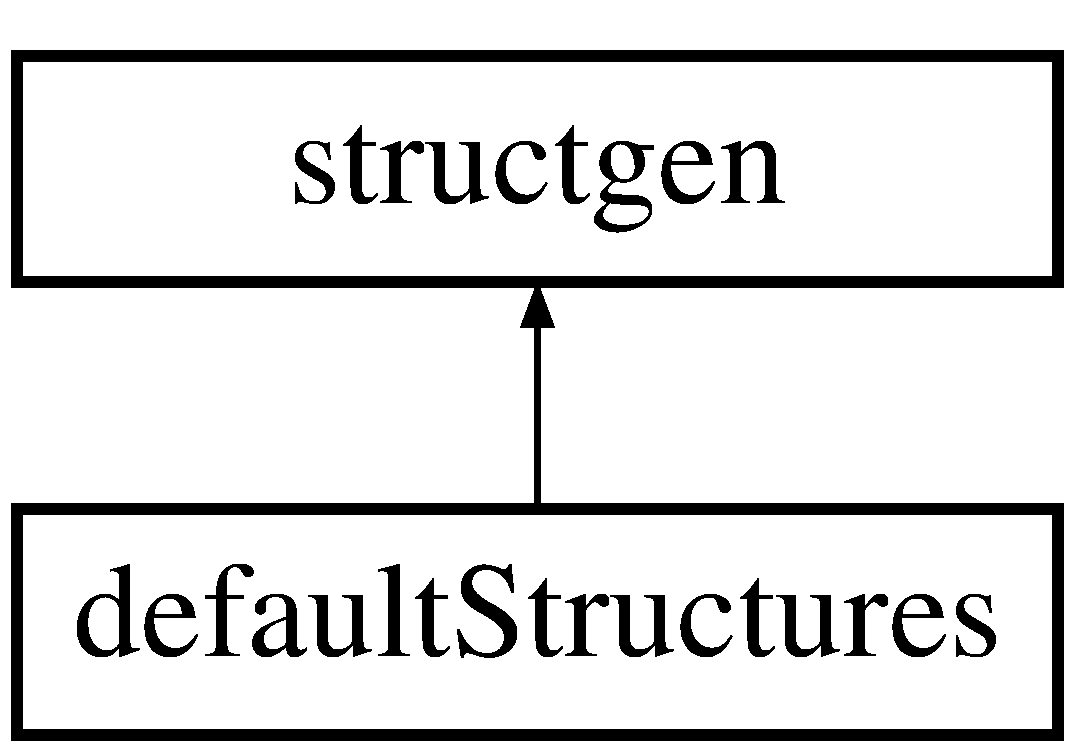
\includegraphics[height=2.000000cm]{classstructgen}
\end{center}
\end{figure}
\subsection*{Public Member Functions}
\begin{DoxyCompactItemize}
\item 
\hypertarget{classstructgen_a36878ba6be584b5b676f7bd98af20ee9}{{\bfseries \-\_\-\-\_\-construct} (\$name, \$mysql\-Object)}\label{classstructgen_a36878ba6be584b5b676f7bd98af20ee9}

\item 
\hyperlink{classstructgen_a92f20c16db5c95fbd705777feacf8125}{create\-Structure} (\$name='\hyperlink{classstructgen}{structgen}')
\item 
\hyperlink{classstructgen_ade4889cf904248b04ad83fbe2f2e74f9}{uni\-Store} (\$name='uni\-Structgen')
\item 
\hyperlink{classstructgen_a9ad9f4819f4914c8f0af701c5d5832e4}{switch\-Structure} (\$name)
\item 
\hyperlink{classstructgen_a68faa951ece5c70b42a9782bcfa3590a}{add} (\$item, \$base=0, \$subnav=null, \$perm=1000, \$link=null, \$priority=null)
\item 
\hyperlink{classstructgen_abe862044c4d94459740b5b6563a4f870}{list\-Structure} ()
\item 
\hyperlink{classstructgen_ad1e438322f50cf6f9cf6025c76ded250}{list\-Base} (\$base)
\end{DoxyCompactItemize}
\subsection*{Protected Attributes}
\begin{DoxyCompactItemize}
\item 
\hypertarget{classstructgen_a6efc15b5a2314dd4b5aaa556a375c6d6}{{\bfseries \$data} =array()}\label{classstructgen_a6efc15b5a2314dd4b5aaa556a375c6d6}

\item 
\hypertarget{classstructgen_a047170d6020a882807665812a27e2525}{{\bfseries \$sql}}\label{classstructgen_a047170d6020a882807665812a27e2525}

\item 
\hypertarget{classstructgen_af28a2bf1bdf5c6f3ffeb459f2bba572b}{{\bfseries \$base\-Ctr}}\label{classstructgen_af28a2bf1bdf5c6f3ffeb459f2bba572b}

\item 
\hypertarget{classstructgen_a629dff33e6ad4aecc6c382d488cdcb08}{{\bfseries \$sub\-Ctr}}\label{classstructgen_a629dff33e6ad4aecc6c382d488cdcb08}

\item 
\hypertarget{classstructgen_ab2fc40d43824ea3e1ce5d86dee0d763b}{{\bfseries \$name}}\label{classstructgen_ab2fc40d43824ea3e1ce5d86dee0d763b}

\end{DoxyCompactItemize}


\subsection{Detailed Description}


Definition at line 11 of file structure.\-generator.\-structgen.\-php.



\subsection{Member Function Documentation}
\hypertarget{classstructgen_a68faa951ece5c70b42a9782bcfa3590a}{\index{structgen@{structgen}!add@{add}}
\index{add@{add}!structgen@{structgen}}
\subsubsection[{add}]{\setlength{\rightskip}{0pt plus 5cm}add (
\begin{DoxyParamCaption}
\item[{}]{\$item, }
\item[{}]{\$base = {\ttfamily 0}, }
\item[{}]{\$subnav = {\ttfamily null}, }
\item[{}]{\$perm = {\ttfamily 1000}, }
\item[{}]{\$link = {\ttfamily null}, }
\item[{}]{\$priority = {\ttfamily null}}
\end{DoxyParamCaption}
)}}\label{classstructgen_a68faa951ece5c70b42a9782bcfa3590a}
Add item / record to structure 
\begin{DoxyParams}{Parameters}
{\em \$item} & string name of item \\
\hline
{\em \$base} & int id of parent (root base is 0) \\
\hline
{\em \$subnav} & int id of new item \\
\hline
{\em \$perm} & int permission for view \\
\hline
{\em \$link} & string full U\-R\-L \\
\hline
{\em \$priority} & int priority level \\
\hline
\end{DoxyParams}


Definition at line 123 of file structure.\-generator.\-structgen.\-php.

\hypertarget{classstructgen_a92f20c16db5c95fbd705777feacf8125}{\index{structgen@{structgen}!create\-Structure@{create\-Structure}}
\index{create\-Structure@{create\-Structure}!structgen@{structgen}}
\subsubsection[{create\-Structure}]{\setlength{\rightskip}{0pt plus 5cm}create\-Structure (
\begin{DoxyParamCaption}
\item[{}]{\$name = {\ttfamily '{\bf structgen}'}}
\end{DoxyParamCaption}
)}}\label{classstructgen_a92f20c16db5c95fbd705777feacf8125}
Create structure 
\begin{DoxyParams}{Parameters}
{\em \$name} & string \\
\hline
\end{DoxyParams}


Definition at line 28 of file structure.\-generator.\-structgen.\-php.

\hypertarget{classstructgen_ad1e438322f50cf6f9cf6025c76ded250}{\index{structgen@{structgen}!list\-Base@{list\-Base}}
\index{list\-Base@{list\-Base}!structgen@{structgen}}
\subsubsection[{list\-Base}]{\setlength{\rightskip}{0pt plus 5cm}list\-Base (
\begin{DoxyParamCaption}
\item[{}]{\$base}
\end{DoxyParamCaption}
)}}\label{classstructgen_ad1e438322f50cf6f9cf6025c76ded250}
List all structure information for one base (for one level) 
\begin{DoxyParams}{Parameters}
{\em \$base} & int \\
\hline
\end{DoxyParams}
\begin{DoxyReturn}{Returns}
array 
\end{DoxyReturn}


Definition at line 183 of file structure.\-generator.\-structgen.\-php.

\hypertarget{classstructgen_abe862044c4d94459740b5b6563a4f870}{\index{structgen@{structgen}!list\-Structure@{list\-Structure}}
\index{list\-Structure@{list\-Structure}!structgen@{structgen}}
\subsubsection[{list\-Structure}]{\setlength{\rightskip}{0pt plus 5cm}list\-Structure (
\begin{DoxyParamCaption}
{}
\end{DoxyParamCaption}
)}}\label{classstructgen_abe862044c4d94459740b5b6563a4f870}
List structure 
\begin{DoxyParams}{Parameters}
{\em \$rootbase} & int \\
\hline
{\em \$maxbase} & int \\
\hline
\end{DoxyParams}


Definition at line 159 of file structure.\-generator.\-structgen.\-php.

\hypertarget{classstructgen_a9ad9f4819f4914c8f0af701c5d5832e4}{\index{structgen@{structgen}!switch\-Structure@{switch\-Structure}}
\index{switch\-Structure@{switch\-Structure}!structgen@{structgen}}
\subsubsection[{switch\-Structure}]{\setlength{\rightskip}{0pt plus 5cm}switch\-Structure (
\begin{DoxyParamCaption}
\item[{}]{\$name}
\end{DoxyParamCaption}
)}}\label{classstructgen_a9ad9f4819f4914c8f0af701c5d5832e4}
Switch to other structure by name 
\begin{DoxyParams}{Parameters}
{\em \$name} & string \\
\hline
\end{DoxyParams}


Definition at line 109 of file structure.\-generator.\-structgen.\-php.

\hypertarget{classstructgen_ade4889cf904248b04ad83fbe2f2e74f9}{\index{structgen@{structgen}!uni\-Store@{uni\-Store}}
\index{uni\-Store@{uni\-Store}!structgen@{structgen}}
\subsubsection[{uni\-Store}]{\setlength{\rightskip}{0pt plus 5cm}uni\-Store (
\begin{DoxyParamCaption}
\item[{}]{\$name = {\ttfamily 'uniStructgen'}}
\end{DoxyParamCaption}
)}}\label{classstructgen_ade4889cf904248b04ad83fbe2f2e74f9}
Create unistore list structure 
\begin{DoxyParams}{Parameters}
{\em \$name} & string \\
\hline
\end{DoxyParams}


Definition at line 64 of file structure.\-generator.\-structgen.\-php.



The documentation for this class was generated from the following file\-:\begin{DoxyCompactItemize}
\item 
/home/peter/git/\-Open\-Sencillo/fw\-\_\-libraries/structure.\-generator.\-structgen.\-php\end{DoxyCompactItemize}

\hypertarget{classtranslate}{\section{translate Class Reference}
\label{classtranslate}\index{translate@{translate}}
}
Inheritance diagram for translate\-:\begin{figure}[H]
\begin{center}
\leavevmode
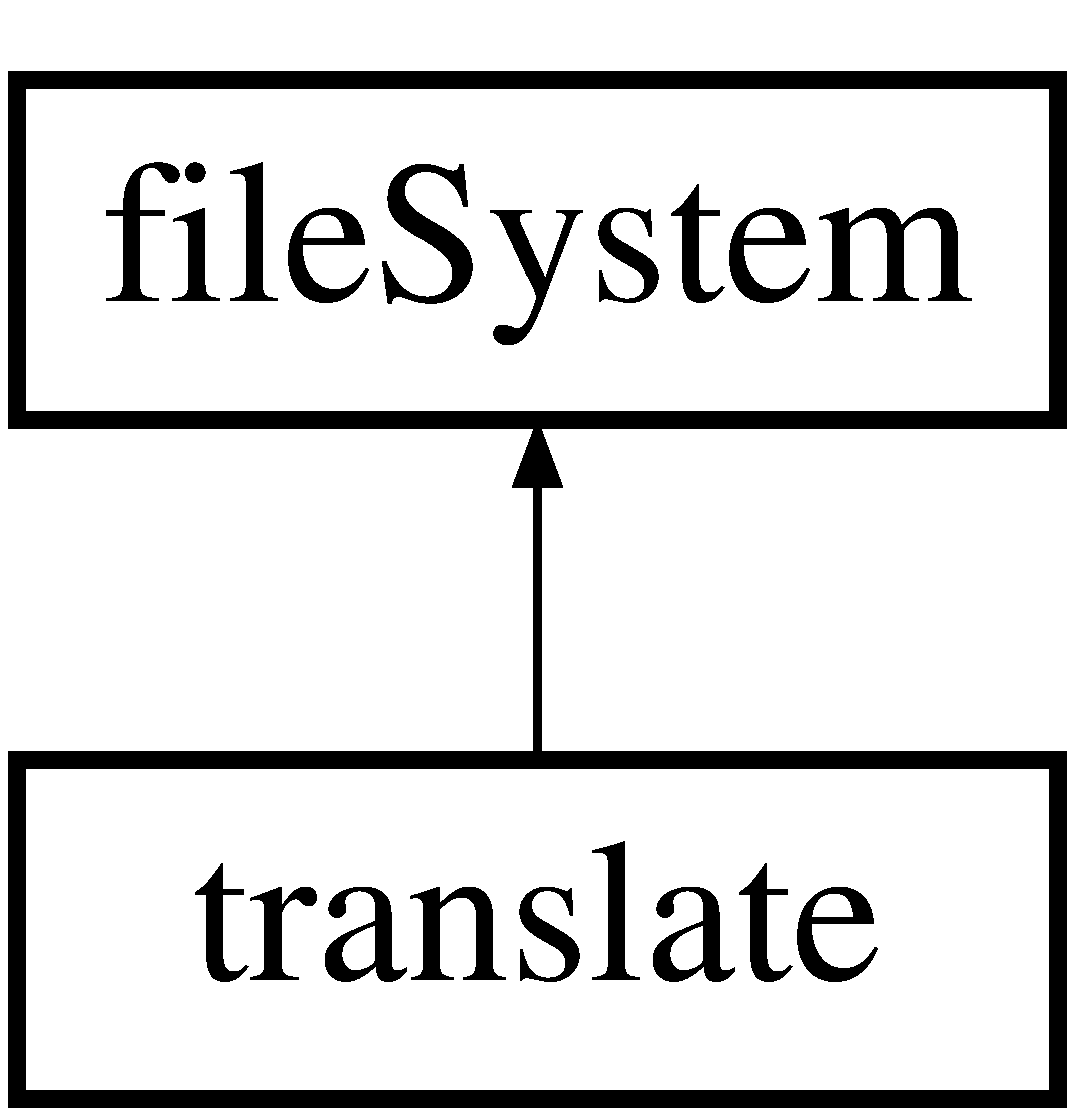
\includegraphics[height=2.000000cm]{classtranslate}
\end{center}
\end{figure}
\subsection*{Public Member Functions}
\begin{DoxyCompactItemize}
\item 
\hypertarget{classtranslate_afa2489379aace6afacf1391038f04fed}{{\bfseries \-\_\-\-\_\-construct} (\$name, \$lang)}\label{classtranslate_afa2489379aace6afacf1391038f04fed}

\item 
\hyperlink{classtranslate_a413ddf994d1d740bb68c2fecfa47e68e}{translate} (\$t\-Key)
\item 
\hypertarget{classtranslate_a2df21f2e384deb0f4f0f42c0ecd069ba}{{\bfseries add\-Translate} (\$t\-Key, \$t\-Data)}\label{classtranslate_a2df21f2e384deb0f4f0f42c0ecd069ba}

\end{DoxyCompactItemize}
\subsection*{Protected Attributes}
\begin{DoxyCompactItemize}
\item 
\hypertarget{classtranslate_a9a663ee008f29e190f7a56c35ae011db}{{\bfseries \$t\-Source}}\label{classtranslate_a9a663ee008f29e190f7a56c35ae011db}

\item 
\hypertarget{classtranslate_a7714b111b644017933931ec69a154102}{{\bfseries \$lang}}\label{classtranslate_a7714b111b644017933931ec69a154102}

\end{DoxyCompactItemize}
\subsection*{Additional Inherited Members}


\subsection{Detailed Description}


Definition at line 12 of file translate.\-tool.\-framework.\-php.



\subsection{Member Function Documentation}
\hypertarget{classtranslate_a413ddf994d1d740bb68c2fecfa47e68e}{\index{translate@{translate}!translate@{translate}}
\index{translate@{translate}!translate@{translate}}
\subsubsection[{translate}]{\setlength{\rightskip}{0pt plus 5cm}{\bf translate} (
\begin{DoxyParamCaption}
\item[{}]{\$t\-Key}
\end{DoxyParamCaption}
)\hspace{0.3cm}{\ttfamily [final]}}}\label{classtranslate_a413ddf994d1d740bb68c2fecfa47e68e}
Find translate by key 
\begin{DoxyParams}[1]{Parameters}
string & {\em \$t\-Key} & \\
\hline
\end{DoxyParams}
\begin{DoxyReturn}{Returns}
bool 
\end{DoxyReturn}


Definition at line 33 of file translate.\-tool.\-framework.\-php.



The documentation for this class was generated from the following file\-:\begin{DoxyCompactItemize}
\item 
/home/peter/git/\-Open\-Sencillo/fw\-\_\-libraries/translate.\-tool.\-framework.\-php\end{DoxyCompactItemize}

\hypertarget{classunit_test}{\section{unit\-Test Class Reference}
\label{classunit_test}\index{unit\-Test@{unit\-Test}}
}
Inheritance diagram for unit\-Test\-:\begin{figure}[H]
\begin{center}
\leavevmode
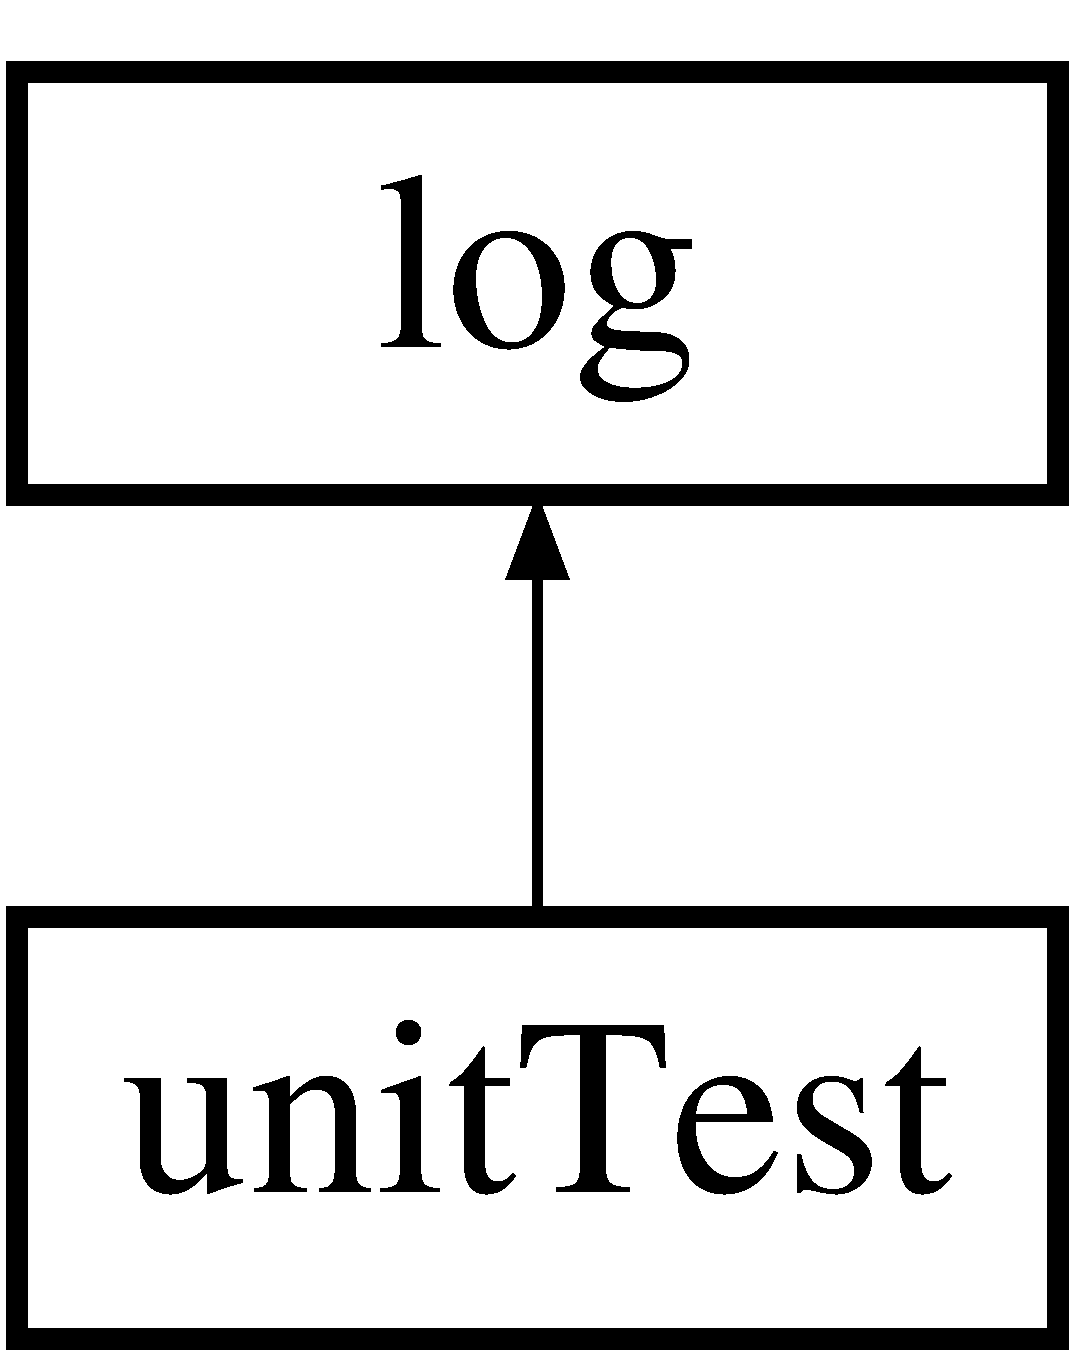
\includegraphics[height=2.000000cm]{classunit_test}
\end{center}
\end{figure}
\subsection*{Public Member Functions}
\begin{DoxyCompactItemize}
\item 
\hyperlink{classunit_test_a87d56f544f853dec06cbd953c3ede752}{set\-Environment} (\$public=true)
\item 
\hypertarget{classunit_test_a2f7869c20ba14e4ccc0b4a70747626e7}{{\bfseries print\-\_\-test} (\$function=null, \$validator=null, \$die=false)}\label{classunit_test_a2f7869c20ba14e4ccc0b4a70747626e7}

\item 
\hypertarget{classunit_test_ae333c4e62083e087bce97578113b2b17}{{\bfseries init} (\$function=null, \$validator=null)}\label{classunit_test_ae333c4e62083e087bce97578113b2b17}

\item 
\hyperlink{classunit_test_a558679772c5cec30a0bb089041a0f430}{print\-\_\-ut} (\$export, \$die=true)
\end{DoxyCompactItemize}
\subsection*{Protected Attributes}
\begin{DoxyCompactItemize}
\item 
\hypertarget{classunit_test_aa99ce9ae015e958eef5782267276fbb4}{{\bfseries \$env} ='public'}\label{classunit_test_aa99ce9ae015e958eef5782267276fbb4}

\end{DoxyCompactItemize}


\subsection{Detailed Description}


Definition at line 132 of file test.\-tool.\-framework.\-php.



\subsection{Member Function Documentation}
\hypertarget{classunit_test_a558679772c5cec30a0bb089041a0f430}{\index{unit\-Test@{unit\-Test}!print\-\_\-ut@{print\-\_\-ut}}
\index{print\-\_\-ut@{print\-\_\-ut}!unitTest@{unit\-Test}}
\subsubsection[{print\-\_\-ut}]{\setlength{\rightskip}{0pt plus 5cm}print\-\_\-ut (
\begin{DoxyParamCaption}
\item[{}]{\$export, }
\item[{}]{\$die = {\ttfamily true}}
\end{DoxyParamCaption}
)}}\label{classunit_test_a558679772c5cec30a0bb089041a0f430}
Create var\-\_\-dump 
\begin{DoxyParams}{Parameters}
{\em mixed} & \\
\hline
\end{DoxyParams}


Definition at line 358 of file test.\-tool.\-framework.\-php.

\hypertarget{classunit_test_a87d56f544f853dec06cbd953c3ede752}{\index{unit\-Test@{unit\-Test}!set\-Environment@{set\-Environment}}
\index{set\-Environment@{set\-Environment}!unitTest@{unit\-Test}}
\subsubsection[{set\-Environment}]{\setlength{\rightskip}{0pt plus 5cm}set\-Environment (
\begin{DoxyParamCaption}
\item[{}]{\$public = {\ttfamily true}}
\end{DoxyParamCaption}
)}}\label{classunit_test_a87d56f544f853dec06cbd953c3ede752}
Setting for switch environment to public or developers


\begin{DoxyParams}{Parameters}
{\em bool$\vert$string} & \\
\hline
\end{DoxyParams}
\begin{DoxyReturn}{Returns}
mixed 
\end{DoxyReturn}


Definition at line 143 of file test.\-tool.\-framework.\-php.



The documentation for this class was generated from the following file\-:\begin{DoxyCompactItemize}
\item 
/home/peter/git/\-Open\-Sencillo/fw\-\_\-libraries/test.\-tool.\-framework.\-php\end{DoxyCompactItemize}

\hypertarget{classupload}{\section{upload Class Reference}
\label{classupload}\index{upload@{upload}}
}
\subsection*{Public Member Functions}
\begin{DoxyCompactItemize}
\item 
\hypertarget{classupload_a03853ceaa393e487835b287de58aba5a}{{\bfseries \-\_\-\-\_\-construct} (\$\hyperlink{classupload_a252353d1d7a5daf38f93859bc7dccccf}{path})}\label{classupload_a03853ceaa393e487835b287de58aba5a}

\item 
\hyperlink{classupload_a186afde49d0e262c66f8f5bdefe42cb4}{mime\-Config} (\$mime=null)
\item 
\hyperlink{classupload_a252353d1d7a5daf38f93859bc7dccccf}{path} (\$path)
\item 
\hyperlink{classupload_a8496ccdff0c6ca5869aa5cf6d0adf7fc}{max\-Size} (\$size)
\item 
\hyperlink{classupload_a5703de110a95a505c2ffd20a1627da89}{advanced\-Mode} (\$mode=null)
\item 
\hyperlink{classupload_ab22a9068029ed1bb11aa9e0cd62bc434}{ajax\-Send\-Json} (\$respond=null)
\item 
\hyperlink{classupload_a4b516aaa5fa38da4fed24ab6001627e2}{name} ()
\item 
\hyperlink{classupload_a160ae63d11b56d3190b172facb43a343}{upload} ()
\end{DoxyCompactItemize}
\subsection*{Protected Member Functions}
\begin{DoxyCompactItemize}
\item 
\hyperlink{classupload_aa9622d0f468253f04aa122505a089a86}{mime\-Test} (\$mime)
\end{DoxyCompactItemize}
\subsection*{Protected Attributes}
\begin{DoxyCompactItemize}
\item 
\hypertarget{classupload_a958cf7aca45cea5359ba0fa80ee2f2c1}{{\bfseries \$mime}}\label{classupload_a958cf7aca45cea5359ba0fa80ee2f2c1}

\item 
\hypertarget{classupload_a0226b5fa357adcccf3ab459aaf3f8631}{{\bfseries \$upload\-Directory}}\label{classupload_a0226b5fa357adcccf3ab459aaf3f8631}

\item 
\hypertarget{classupload_af594986e4618a8d6a5d7566617f583c6}{{\bfseries \$size}}\label{classupload_af594986e4618a8d6a5d7566617f583c6}

\item 
\hypertarget{classupload_a430a2c99398e101d3e3ed06a18480b87}{{\bfseries \$upload\-Info}}\label{classupload_a430a2c99398e101d3e3ed06a18480b87}

\item 
\hypertarget{classupload_a3aaf40baac36e278c7d7c9139df1750c}{{\bfseries \$mode}}\label{classupload_a3aaf40baac36e278c7d7c9139df1750c}

\item 
\hypertarget{classupload_a58391ea75f2d29d5d708d7050b641c33}{{\bfseries \$status}}\label{classupload_a58391ea75f2d29d5d708d7050b641c33}

\end{DoxyCompactItemize}


\subsection{Detailed Description}


Definition at line 11 of file files.\-upload.\-fup.\-php.



\subsection{Member Function Documentation}
\hypertarget{classupload_a5703de110a95a505c2ffd20a1627da89}{\index{upload@{upload}!advanced\-Mode@{advanced\-Mode}}
\index{advanced\-Mode@{advanced\-Mode}!upload@{upload}}
\subsubsection[{advanced\-Mode}]{\setlength{\rightskip}{0pt plus 5cm}advanced\-Mode (
\begin{DoxyParamCaption}
\item[{}]{\$mode = {\ttfamily null}}
\end{DoxyParamCaption}
)}}\label{classupload_a5703de110a95a505c2ffd20a1627da89}
Advanced upload mode T\-R\-U\-E/\-F\-A\-L\-S\-E, deafult F\-A\-L\-S\-E


\begin{DoxyParams}[1]{Parameters}
bool & {\em \$mode} & \\
\hline
\end{DoxyParams}


Definition at line 93 of file files.\-upload.\-fup.\-php.

\hypertarget{classupload_ab22a9068029ed1bb11aa9e0cd62bc434}{\index{upload@{upload}!ajax\-Send\-Json@{ajax\-Send\-Json}}
\index{ajax\-Send\-Json@{ajax\-Send\-Json}!upload@{upload}}
\subsubsection[{ajax\-Send\-Json}]{\setlength{\rightskip}{0pt plus 5cm}ajax\-Send\-Json (
\begin{DoxyParamCaption}
\item[{}]{\$respond = {\ttfamily null}}
\end{DoxyParamCaption}
)\hspace{0.3cm}{\ttfamily [final]}}}\label{classupload_ab22a9068029ed1bb11aa9e0cd62bc434}
Json status encoder for A\-J\-A\-X comunication 

Definition at line 109 of file files.\-upload.\-fup.\-php.

\hypertarget{classupload_a8496ccdff0c6ca5869aa5cf6d0adf7fc}{\index{upload@{upload}!max\-Size@{max\-Size}}
\index{max\-Size@{max\-Size}!upload@{upload}}
\subsubsection[{max\-Size}]{\setlength{\rightskip}{0pt plus 5cm}max\-Size (
\begin{DoxyParamCaption}
\item[{}]{\$size}
\end{DoxyParamCaption}
)}}\label{classupload_a8496ccdff0c6ca5869aa5cf6d0adf7fc}
Maximum allowed file size


\begin{DoxyParams}[1]{Parameters}
int & {\em \$size} & \\
\hline
\end{DoxyParams}


Definition at line 83 of file files.\-upload.\-fup.\-php.

\hypertarget{classupload_a186afde49d0e262c66f8f5bdefe42cb4}{\index{upload@{upload}!mime\-Config@{mime\-Config}}
\index{mime\-Config@{mime\-Config}!upload@{upload}}
\subsubsection[{mime\-Config}]{\setlength{\rightskip}{0pt plus 5cm}mime\-Config (
\begin{DoxyParamCaption}
\item[{}]{\$mime = {\ttfamily null}}
\end{DoxyParamCaption}
)}}\label{classupload_a186afde49d0e262c66f8f5bdefe42cb4}
Config method for legal mime types


\begin{DoxyParams}[1]{Parameters}
string & {\em \$mime} & \\
\hline
\end{DoxyParams}
default, if \$mime is null

Definition at line 45 of file files.\-upload.\-fup.\-php.

\hypertarget{classupload_aa9622d0f468253f04aa122505a089a86}{\index{upload@{upload}!mime\-Test@{mime\-Test}}
\index{mime\-Test@{mime\-Test}!upload@{upload}}
\subsubsection[{mime\-Test}]{\setlength{\rightskip}{0pt plus 5cm}mime\-Test (
\begin{DoxyParamCaption}
\item[{}]{\$mime}
\end{DoxyParamCaption}
)\hspace{0.3cm}{\ttfamily [protected]}}}\label{classupload_aa9622d0f468253f04aa122505a089a86}
Internal protected function for detection legal mime type


\begin{DoxyParams}[1]{Parameters}
mixed & {\em \$mime} & \\
\hline
\end{DoxyParams}


Definition at line 32 of file files.\-upload.\-fup.\-php.

\hypertarget{classupload_a4b516aaa5fa38da4fed24ab6001627e2}{\index{upload@{upload}!name@{name}}
\index{name@{name}!upload@{upload}}
\subsubsection[{name}]{\setlength{\rightskip}{0pt plus 5cm}name (
\begin{DoxyParamCaption}
{}
\end{DoxyParamCaption}
)}}\label{classupload_a4b516aaa5fa38da4fed24ab6001627e2}
Get new file name 

Definition at line 124 of file files.\-upload.\-fup.\-php.

\hypertarget{classupload_a252353d1d7a5daf38f93859bc7dccccf}{\index{upload@{upload}!path@{path}}
\index{path@{path}!upload@{upload}}
\subsubsection[{path}]{\setlength{\rightskip}{0pt plus 5cm}path (
\begin{DoxyParamCaption}
\item[{}]{\$path}
\end{DoxyParamCaption}
)}}\label{classupload_a252353d1d7a5daf38f93859bc7dccccf}
specify upload directory ends with / (slash)


\begin{DoxyParams}[1]{Parameters}
string & {\em \$path} & \\
\hline
\end{DoxyParams}


Definition at line 73 of file files.\-upload.\-fup.\-php.

\hypertarget{classupload_a160ae63d11b56d3190b172facb43a343}{\index{upload@{upload}!upload@{upload}}
\index{upload@{upload}!upload@{upload}}
\subsubsection[{upload}]{\setlength{\rightskip}{0pt plus 5cm}{\bf upload} (
\begin{DoxyParamCaption}
{}
\end{DoxyParamCaption}
)}}\label{classupload_a160ae63d11b56d3190b172facb43a343}
Upload method

200 -\/ O\-K 404 -\/ Not found / Unknown error / No file 413 -\/ Request is to large (maximum size is low) 415-\/0 -\/ Unsupported Media Type (acquired in upload method) 415-\/1 -\/ Unsupported Media Type (acquired in mime\-Config method) 417 -\/ Expectation Failed (failed moving file from temporary location) 444 -\/ No Response / Internal A\-J\-A\-X fail 

Definition at line 140 of file files.\-upload.\-fup.\-php.



The documentation for this class was generated from the following file\-:\begin{DoxyCompactItemize}
\item 
/home/peter/git/\-Open\-Sencillo/fw\-\_\-libraries/files.\-upload.\-fup.\-php\end{DoxyCompactItemize}

\hypertarget{classurl}{\section{url Class Reference}
\label{classurl}\index{url@{url}}
}
\subsection*{Public Member Functions}
\begin{DoxyCompactItemize}
\item 
\hyperlink{classurl_ac3ad0a893ce447a4b92b7bea59371f02}{url} (\$array=false)
\item 
\hyperlink{classurl_ab302f269413f4e58217d5801cd52ca39}{add\-Url} (\$\hyperlink{classurl}{url}, \$template)
\item 
\hyperlink{classurl_a3022830a582288c8216b5cbfaed1dec7}{remove\-Url} (\$\hyperlink{classurl}{url})
\item 
\hypertarget{classurl_a259aafa22bfa702c4309ab5bbf975f78}{{\bfseries get\-Page} (\$page)}\label{classurl_a259aafa22bfa702c4309ab5bbf975f78}

\item 
\hyperlink{classurl_ad78ae85a173fbd81e6668608a1c49106}{breadcrumb} (\$page, \$page\-Names)
\end{DoxyCompactItemize}
\subsection*{Protected Attributes}
\begin{DoxyCompactItemize}
\item 
\hypertarget{classurl_a6efc15b5a2314dd4b5aaa556a375c6d6}{{\bfseries \$data}}\label{classurl_a6efc15b5a2314dd4b5aaa556a375c6d6}

\end{DoxyCompactItemize}


\subsection{Detailed Description}


Definition at line 12 of file url.\-management.\-urlman.\-php.



\subsection{Member Function Documentation}
\hypertarget{classurl_ab302f269413f4e58217d5801cd52ca39}{\index{url@{url}!add\-Url@{add\-Url}}
\index{add\-Url@{add\-Url}!url@{url}}
\subsubsection[{add\-Url}]{\setlength{\rightskip}{0pt plus 5cm}add\-Url (
\begin{DoxyParamCaption}
\item[{}]{\$url, }
\item[{}]{\$template}
\end{DoxyParamCaption}
)}}\label{classurl_ab302f269413f4e58217d5801cd52ca39}
Add url 
\begin{DoxyParams}{Parameters}
{\em string} & relative page url \\
\hline
{\em string} & file template url \\
\hline
\end{DoxyParams}


Definition at line 36 of file url.\-management.\-urlman.\-php.

\hypertarget{classurl_ad78ae85a173fbd81e6668608a1c49106}{\index{url@{url}!breadcrumb@{breadcrumb}}
\index{breadcrumb@{breadcrumb}!url@{url}}
\subsubsection[{breadcrumb}]{\setlength{\rightskip}{0pt plus 5cm}breadcrumb (
\begin{DoxyParamCaption}
\item[{}]{\$page, }
\item[{}]{\$page\-Names}
\end{DoxyParamCaption}
)}}\label{classurl_ad78ae85a173fbd81e6668608a1c49106}
Breadcrumb select 
\begin{DoxyParams}{Parameters}
{\em string} & from P\-A\-G\-E \\
\hline
{\em array('ab/cd/ef'=$>$'\-Ef} & page')\\
\hline
\end{DoxyParams}
\$this-\/$>$breadcrumb(P\-A\-G\-E,array('first'=$>$'My first page','first/second'=$>$'My second page','first/second/third'=$>$'My third page'));

\begin{DoxyReturn}{Returns}
array(0=$>$'Page name 0',1=$>$'Page name 1' ...) 
\end{DoxyReturn}


Definition at line 69 of file url.\-management.\-urlman.\-php.

\hypertarget{classurl_a3022830a582288c8216b5cbfaed1dec7}{\index{url@{url}!remove\-Url@{remove\-Url}}
\index{remove\-Url@{remove\-Url}!url@{url}}
\subsubsection[{remove\-Url}]{\setlength{\rightskip}{0pt plus 5cm}remove\-Url (
\begin{DoxyParamCaption}
\item[{}]{\$url}
\end{DoxyParamCaption}
)}}\label{classurl_a3022830a582288c8216b5cbfaed1dec7}
Remove url 
\begin{DoxyParams}{Parameters}
{\em string} & \\
\hline
\end{DoxyParams}


Definition at line 45 of file url.\-management.\-urlman.\-php.

\hypertarget{classurl_ac3ad0a893ce447a4b92b7bea59371f02}{\index{url@{url}!url@{url}}
\index{url@{url}!url@{url}}
\subsubsection[{url}]{\setlength{\rightskip}{0pt plus 5cm}{\bf url} (
\begin{DoxyParamCaption}
\item[{}]{\$array = {\ttfamily false}}
\end{DoxyParamCaption}
)}}\label{classurl_ac3ad0a893ce447a4b92b7bea59371f02}
Get url/urls 
\begin{DoxyParams}{Parameters}
{\em bool} & \\
\hline
\end{DoxyParams}
\begin{DoxyReturn}{Returns}
mixed 
\end{DoxyReturn}


Definition at line 26 of file url.\-management.\-urlman.\-php.



The documentation for this class was generated from the following file\-:\begin{DoxyCompactItemize}
\item 
/home/peter/git/\-Open\-Sencillo/fw\-\_\-libraries/url.\-management.\-urlman.\-php\end{DoxyCompactItemize}

\hypertarget{class_user_agent_parser}{\section{User\-Agent\-Parser Class Reference}
\label{class_user_agent_parser}\index{User\-Agent\-Parser@{User\-Agent\-Parser}}
}
\subsection*{Static Public Member Functions}
\begin{DoxyCompactItemize}
\item 
static \hyperlink{class_user_agent_parser_ac435f3d1806cea069a6ca890ab1883c4}{get\-Operating\-System} (\$user\-Agent)
\item 
static \hyperlink{class_user_agent_parser_a54038e0276f884046a26514fd9c262b0}{get\-Browser} (\$user\-Agent)
\item 
\hypertarget{class_user_agent_parser_a62a7a74fe088a35b3f233bf67df2012b}{static {\bfseries get\-Browser\-Name\-From\-Id} (\$browser\-Id)}\label{class_user_agent_parser_a62a7a74fe088a35b3f233bf67df2012b}

\item 
\hypertarget{class_user_agent_parser_a5223fe564aa5f8872c1ad03e2c868b44}{static {\bfseries get\-Browser\-Short\-Name\-From\-Id} (\$browser\-Id)}\label{class_user_agent_parser_a5223fe564aa5f8872c1ad03e2c868b44}

\item 
\hypertarget{class_user_agent_parser_ada5bf3c372bdeafe45c06a5bca1a7cb3}{static {\bfseries get\-Browser\-Family\-From\-Id} (\$browser\-Id)}\label{class_user_agent_parser_ada5bf3c372bdeafe45c06a5bca1a7cb3}

\item 
\hypertarget{class_user_agent_parser_a654d56eac9925308282304e98b6b981e}{static {\bfseries get\-Operating\-System\-Name\-From\-Id} (\$os\-Id)}\label{class_user_agent_parser_a654d56eac9925308282304e98b6b981e}

\item 
\hypertarget{class_user_agent_parser_a0def641c9d57aa4cb3b89672cde82884}{static {\bfseries get\-Operating\-System\-Short\-Name\-From\-Id} (\$os\-Id)}\label{class_user_agent_parser_a0def641c9d57aa4cb3b89672cde82884}

\item 
\hypertarget{class_user_agent_parser_a4a677f5103ebf2631c940c06384adfe4}{static {\bfseries get\-Operating\-System\-Id\-From\-Name} (\$os\-Name)}\label{class_user_agent_parser_a4a677f5103ebf2631c940c06384adfe4}

\item 
\hypertarget{class_user_agent_parser_a7e5b3840ca6c0e2081ac3f41eece3c4e}{static {\bfseries get\-Operating\-System\-Family\-From\-Id} (\$os\-Id)}\label{class_user_agent_parser_a7e5b3840ca6c0e2081ac3f41eece3c4e}

\end{DoxyCompactItemize}
\subsection*{Static Protected Member Functions}
\begin{DoxyCompactItemize}
\item 
\hypertarget{class_user_agent_parser_add41e0ac3852ff63f876e5b04fedc069}{static {\bfseries cleanup\-User\-Agent} (\$user\-Agent)}\label{class_user_agent_parser_add41e0ac3852ff63f876e5b04fedc069}

\item 
\hypertarget{class_user_agent_parser_a9f0be6ae273d3669e11c29910a0be338}{static {\bfseries init} ()}\label{class_user_agent_parser_a9f0be6ae273d3669e11c29910a0be338}

\end{DoxyCompactItemize}
\subsection*{Static Protected Attributes}
\begin{DoxyCompactItemize}
\item 
\hypertarget{class_user_agent_parser_a81edf933083b5ac5b380385f59074a7d}{static {\bfseries \$browsers}}\label{class_user_agent_parser_a81edf933083b5ac5b380385f59074a7d}

\item 
static {\bfseries \$browser\-Type}
\item 
static {\bfseries \$safari\-Versions}
\item 
static {\bfseries \$omni\-Web\-Versions}
\item 
\hypertarget{class_user_agent_parser_a6c81c14f25de6a8b8206335eea724eb1}{static {\bfseries \$operating\-Systems}}\label{class_user_agent_parser_a6c81c14f25de6a8b8206335eea724eb1}

\item 
static {\bfseries \$os\-Type}
\item 
\hypertarget{class_user_agent_parser_a1d8d7fab9e2c2974919888f5b886295e}{static {\bfseries \$browser\-Id\-To\-Name}}\label{class_user_agent_parser_a1d8d7fab9e2c2974919888f5b886295e}

\item 
\hypertarget{class_user_agent_parser_a7958078b2a0013798f14838fa1fd40c1}{static {\bfseries \$browser\-Id\-To\-Short\-Name}}\label{class_user_agent_parser_a7958078b2a0013798f14838fa1fd40c1}

\item 
\hypertarget{class_user_agent_parser_ab68e07510370828435a3e86c320c7bdc}{static {\bfseries \$operating\-Systems\-Id\-To\-Name}}\label{class_user_agent_parser_ab68e07510370828435a3e86c320c7bdc}

\item 
\hypertarget{class_user_agent_parser_ada1762b34d38d7498838252118cca041}{static {\bfseries \$operating\-Systems\-Id\-To\-Short\-Name}}\label{class_user_agent_parser_ada1762b34d38d7498838252118cca041}

\end{DoxyCompactItemize}


\subsection{Detailed Description}


Definition at line 60 of file user\-Agent.\-parser.\-usagpa.\-php.



\subsection{Member Function Documentation}
\hypertarget{class_user_agent_parser_a54038e0276f884046a26514fd9c262b0}{\index{User\-Agent\-Parser@{User\-Agent\-Parser}!get\-Browser@{get\-Browser}}
\index{get\-Browser@{get\-Browser}!UserAgentParser@{User\-Agent\-Parser}}
\subsubsection[{get\-Browser}]{\setlength{\rightskip}{0pt plus 5cm}static get\-Browser (
\begin{DoxyParamCaption}
\item[{}]{\$user\-Agent}
\end{DoxyParamCaption}
)\hspace{0.3cm}{\ttfamily [static]}}}\label{class_user_agent_parser_a54038e0276f884046a26514fd9c262b0}
Returns the browser information array, given a user agent string.


\begin{DoxyParams}[1]{Parameters}
string & {\em \$user\-Agent} & \\
\hline
\end{DoxyParams}
\begin{DoxyReturn}{Returns}
array false if the browser is \char`\"{}unknown\char`\"{}, or array( 'id' =$>$ '', // 2 letters I\-D, eg. F\-F 'name' =$>$ '', // 2 letters I\-D, eg. F\-F 'short\-\_\-name' =$>$ '', // 2 letters I\-D, eg. F\-F 'major\-\_\-number' =$>$ '', // 2 in firefox 2.\-0.\-12 'minor\-\_\-number' =$>$ '', // 0 in firefox 2.\-0.\-12 'version' =$>$ '', // major\-\_\-number.\-minor\-\_\-number ); 
\end{DoxyReturn}
\begin{DoxySeeAlso}{See Also}
self\-::\$browsers for the list of O\-S 
\end{DoxySeeAlso}


Definition at line 361 of file user\-Agent.\-parser.\-usagpa.\-php.

\hypertarget{class_user_agent_parser_ac435f3d1806cea069a6ca890ab1883c4}{\index{User\-Agent\-Parser@{User\-Agent\-Parser}!get\-Operating\-System@{get\-Operating\-System}}
\index{get\-Operating\-System@{get\-Operating\-System}!UserAgentParser@{User\-Agent\-Parser}}
\subsubsection[{get\-Operating\-System}]{\setlength{\rightskip}{0pt plus 5cm}static get\-Operating\-System (
\begin{DoxyParamCaption}
\item[{}]{\$user\-Agent}
\end{DoxyParamCaption}
)\hspace{0.3cm}{\ttfamily [static]}}}\label{class_user_agent_parser_ac435f3d1806cea069a6ca890ab1883c4}
Returns an array of the O\-S for the submitted user agent 'id' =$>$ '', 'name' =$>$ '', 'short\-\_\-name' =$>$ '',


\begin{DoxyParams}[1]{Parameters}
string & {\em \$user\-Agent} & \\
\hline
\end{DoxyParams}
\begin{DoxyReturn}{Returns}
string false if O\-S couldn't be identified, or 3 letters I\-D (eg. W\-X\-P) 
\end{DoxyReturn}
\begin{DoxySeeAlso}{See Also}
User\-Agent\-Parser/\-Operating\-Systems.\-php for the list of O\-S (also available in self\-::\$operating\-Systems) 
\end{DoxySeeAlso}


Definition at line 320 of file user\-Agent.\-parser.\-usagpa.\-php.



\subsection{Field Documentation}
\hypertarget{class_user_agent_parser_ad0821f30ee48c49356b114884ad1c552}{\index{User\-Agent\-Parser@{User\-Agent\-Parser}!\$browser\-Type@{\$browser\-Type}}
\index{\$browser\-Type@{\$browser\-Type}!UserAgentParser@{User\-Agent\-Parser}}
\subsubsection[{\$browser\-Type}]{\setlength{\rightskip}{0pt plus 5cm}\$browser\-Type\hspace{0.3cm}{\ttfamily [static]}, {\ttfamily [protected]}}}\label{class_user_agent_parser_ad0821f30ee48c49356b114884ad1c552}
{\bfseries Initial value\-:}
\begin{DoxyCode}
= array(
        \textcolor{stringliteral}{'ie'}        => array(\textcolor{stringliteral}{'IE'}),
        \textcolor{stringliteral}{'gecko'}     => array(\textcolor{stringliteral}{'NS'}, \textcolor{stringliteral}{'PX'}, \textcolor{stringliteral}{'FF'}, \textcolor{stringliteral}{'FB'}, \textcolor{stringliteral}{'CA'}, \textcolor{stringliteral}{'GA'}, \textcolor{stringliteral}{'KM'}, \textcolor{stringliteral}{'MO'}, \textcolor{stringliteral}{'SM'}, \textcolor{stringliteral}{'CO'}, \textcolor{stringliteral}{'FE'}, \textcolor{stringliteral}{'KP'}, \textcolor{stringliteral}{'KZ'}, \textcolor{stringliteral}{
      'TB'}),
        \textcolor{stringliteral}{'khtml'}     => array(\textcolor{stringliteral}{'KO'}),
        \textcolor{stringliteral}{'webkit'}    => array(\textcolor{stringliteral}{'SF'}, \textcolor{stringliteral}{'CH'}, \textcolor{stringliteral}{'OW'}, \textcolor{stringliteral}{'AR'}, \textcolor{stringliteral}{'EP'}, \textcolor{stringliteral}{'FL'}, \textcolor{stringliteral}{'WO'}, \textcolor{stringliteral}{'AB'}, \textcolor{stringliteral}{'IR'}, \textcolor{stringliteral}{'CS'}, \textcolor{stringliteral}{'FD'}, \textcolor{stringliteral}{'HA'}, \textcolor{stringliteral}{'MI'}, \textcolor{stringliteral}{
      'GE'}, \textcolor{stringliteral}{'DF'}, \textcolor{stringliteral}{'BB'}, \textcolor{stringliteral}{'BP'}, \textcolor{stringliteral}{'TI'}, \textcolor{stringliteral}{'CF'}, \textcolor{stringliteral}{'RK'}, \textcolor{stringliteral}{'B2'}, \textcolor{stringliteral}{'NF'}),
        \textcolor{stringliteral}{'opera'}     => array(\textcolor{stringliteral}{'OP'}),
    )
\end{DoxyCode}


Definition at line 153 of file user\-Agent.\-parser.\-usagpa.\-php.

\hypertarget{class_user_agent_parser_a0f50a04746313e5adeaaa8fe0edcb115}{\index{User\-Agent\-Parser@{User\-Agent\-Parser}!\$omni\-Web\-Versions@{\$omni\-Web\-Versions}}
\index{\$omni\-Web\-Versions@{\$omni\-Web\-Versions}!UserAgentParser@{User\-Agent\-Parser}}
\subsubsection[{\$omni\-Web\-Versions}]{\setlength{\rightskip}{0pt plus 5cm}\$omni\-Web\-Versions\hspace{0.3cm}{\ttfamily [static]}, {\ttfamily [protected]}}}\label{class_user_agent_parser_a0f50a04746313e5adeaaa8fe0edcb115}
{\bfseries Initial value\-:}
\begin{DoxyCode}
= array(
        \textcolor{stringliteral}{'622.15'}    => array(\textcolor{charliteral}{'5'}, \textcolor{stringliteral}{'11'}),
        \textcolor{stringliteral}{'622.10'}    => array(\textcolor{charliteral}{'5'}, \textcolor{stringliteral}{'10'}),
        \textcolor{stringliteral}{'622.8'}     => array(\textcolor{charliteral}{'5'}, \textcolor{charliteral}{'9'}),
        \textcolor{stringliteral}{'622.3'}     => array(\textcolor{charliteral}{'5'}, \textcolor{charliteral}{'8'}),
        \textcolor{stringliteral}{'621'}       => array(\textcolor{charliteral}{'5'}, \textcolor{charliteral}{'7'}),
        \textcolor{stringliteral}{'613'}       => array(\textcolor{charliteral}{'5'}, \textcolor{charliteral}{'6'}),
        \textcolor{stringliteral}{'607'}       => array(\textcolor{charliteral}{'5'}, \textcolor{charliteral}{'5'}),
        \textcolor{stringliteral}{'563.34'}    => array(\textcolor{charliteral}{'5'}, \textcolor{charliteral}{'1'}),
        \textcolor{stringliteral}{'558.36'}    => array(\textcolor{charliteral}{'5'}, \textcolor{charliteral}{'0'}),
        \textcolor{stringliteral}{'496'}       => array(\textcolor{charliteral}{'4'}, \textcolor{charliteral}{'5'}),
    )
\end{DoxyCode}


Definition at line 179 of file user\-Agent.\-parser.\-usagpa.\-php.

\hypertarget{class_user_agent_parser_a35cddafe55870d08e38ce841e7902a4b}{\index{User\-Agent\-Parser@{User\-Agent\-Parser}!\$os\-Type@{\$os\-Type}}
\index{\$os\-Type@{\$os\-Type}!UserAgentParser@{User\-Agent\-Parser}}
\subsubsection[{\$os\-Type}]{\setlength{\rightskip}{0pt plus 5cm}\$os\-Type\hspace{0.3cm}{\ttfamily [static]}, {\ttfamily [protected]}}}\label{class_user_agent_parser_a35cddafe55870d08e38ce841e7902a4b}
{\bfseries Initial value\-:}
\begin{DoxyCode}
= array(
        \textcolor{stringliteral}{'Windows'}               => array(\textcolor{stringliteral}{'WI8'}, \textcolor{stringliteral}{'WI7'}, \textcolor{stringliteral}{'WVI'}, \textcolor{stringliteral}{'WS3'}, \textcolor{stringliteral}{'WXP'}, \textcolor{stringliteral}{'W2K'}, \textcolor{stringliteral}{'WNT'}, \textcolor{stringliteral}{'WME'}, \textcolor{stringliteral}{'W98'}, \textcolor{stringliteral}{'
      W95'}),
        \textcolor{stringliteral}{'Linux'}                 => array(\textcolor{stringliteral}{'LIN'}),
        \textcolor{stringliteral}{'Mac'}                   => array(\textcolor{stringliteral}{'MAC'}),
        \textcolor{stringliteral}{'iOS'}                   => array(\textcolor{stringliteral}{'IPD'}, \textcolor{stringliteral}{'IPA'}, \textcolor{stringliteral}{'IPH'}),
        \textcolor{stringliteral}{'Android'}               => array(\textcolor{stringliteral}{'AND'}),
        \textcolor{stringliteral}{'Windows Mobile'}        => array(\textcolor{stringliteral}{'WPH'}, \textcolor{stringliteral}{'WMO'}, \textcolor{stringliteral}{'WCE'}),
        \textcolor{stringliteral}{'Gaming Console'}        => array(\textcolor{stringliteral}{'WII'}, \textcolor{stringliteral}{'WIU'}, \textcolor{stringliteral}{'PS3'}, \textcolor{stringliteral}{'XBX'}),
        \textcolor{stringliteral}{'Mobile Gaming Console'} => array(\textcolor{stringliteral}{'PSP'}, \textcolor{stringliteral}{'PSV'}, \textcolor{stringliteral}{'NDS'}, \textcolor{stringliteral}{'DSI'}, \textcolor{stringliteral}{'3DS'}),
        \textcolor{stringliteral}{'Unix'}                  => array(\textcolor{stringliteral}{'SOS'}, \textcolor{stringliteral}{'AIX'}, \textcolor{stringliteral}{'HP-UX'}, \textcolor{stringliteral}{'BSD'}, \textcolor{stringliteral}{'NBS'}, \textcolor{stringliteral}{'OBS'}, \textcolor{stringliteral}{'DFB'}, \textcolor{stringliteral}{'SYL'}, \textcolor{stringliteral}{'IRI'}, \textcolor{stringliteral}{'
      T64'}),
        \textcolor{stringliteral}{'Other Mobile'}          => array(\textcolor{stringliteral}{'MAE'}, \textcolor{stringliteral}{'WOS'}, \textcolor{stringliteral}{'POS'}, \textcolor{stringliteral}{'BLB'}, \textcolor{stringliteral}{'QNX'}, \textcolor{stringliteral}{'SYM'}, \textcolor{stringliteral}{'SBA'}),
        \textcolor{stringliteral}{'Other'}                 => array(\textcolor{stringliteral}{'VMS'}, \textcolor{stringliteral}{'OS2'}, \textcolor{stringliteral}{'BEOS'}, \textcolor{stringliteral}{'AMI'})
    )
\end{DoxyCode}


Definition at line 292 of file user\-Agent.\-parser.\-usagpa.\-php.

\hypertarget{class_user_agent_parser_a3493595b0af2ff79e44fe73847a67688}{\index{User\-Agent\-Parser@{User\-Agent\-Parser}!\$safari\-Versions@{\$safari\-Versions}}
\index{\$safari\-Versions@{\$safari\-Versions}!UserAgentParser@{User\-Agent\-Parser}}
\subsubsection[{\$safari\-Versions}]{\setlength{\rightskip}{0pt plus 5cm}\$safari\-Versions\hspace{0.3cm}{\ttfamily [static]}, {\ttfamily [protected]}}}\label{class_user_agent_parser_a3493595b0af2ff79e44fe73847a67688}
{\bfseries Initial value\-:}
\begin{DoxyCode}
= array(
        \textcolor{stringliteral}{'536.25'}    => array(\textcolor{charliteral}{'6'}, \textcolor{charliteral}{'0'}),
        \textcolor{stringliteral}{'534.48'}    => array(\textcolor{charliteral}{'5'}, \textcolor{charliteral}{'1'}),
        \textcolor{stringliteral}{'533.16'}    => array(\textcolor{charliteral}{'5'}, \textcolor{charliteral}{'0'}),
        \textcolor{stringliteral}{'533.4'}     => array(\textcolor{charliteral}{'4'}, \textcolor{charliteral}{'1'}),
        \textcolor{stringliteral}{'526.11.2'}  => array(\textcolor{charliteral}{'4'}, \textcolor{charliteral}{'0'}),
        \textcolor{stringliteral}{'525.26'}    => array(\textcolor{charliteral}{'3'}, \textcolor{charliteral}{'2'}),
        \textcolor{stringliteral}{'525.13'}    => array(\textcolor{charliteral}{'3'}, \textcolor{charliteral}{'1'}),
        \textcolor{stringliteral}{'522.11'}    => array(\textcolor{charliteral}{'3'}, \textcolor{charliteral}{'0'}),
        \textcolor{stringliteral}{'412'}       => array(\textcolor{charliteral}{'2'}, \textcolor{charliteral}{'0'}),
        \textcolor{stringliteral}{'312'}       => array(\textcolor{charliteral}{'1'}, \textcolor{charliteral}{'3'}),
        \textcolor{stringliteral}{'125'}       => array(\textcolor{charliteral}{'1'}, \textcolor{charliteral}{'2'}),
        \textcolor{stringliteral}{'100'}       => array(\textcolor{charliteral}{'1'}, \textcolor{charliteral}{'1'}),
        \textcolor{stringliteral}{'85'}        => array(\textcolor{charliteral}{'1'}, \textcolor{charliteral}{'0'}),
        \textcolor{stringliteral}{'73'}        => array(\textcolor{charliteral}{'0'}, \textcolor{charliteral}{'9'}),
        \textcolor{stringliteral}{'48'}        => array(\textcolor{charliteral}{'0'}, \textcolor{charliteral}{'8'}),
    )
\end{DoxyCode}


Definition at line 161 of file user\-Agent.\-parser.\-usagpa.\-php.



The documentation for this class was generated from the following file\-:\begin{DoxyCompactItemize}
\item 
/home/peter/git/\-Open\-Sencillo/fw\-\_\-libraries/user\-Agent.\-parser.\-usagpa.\-php\end{DoxyCompactItemize}

\chapter{Example Documentation}
\hypertarget{array-example}{\section{array}
}
Insert data 
\begin{DoxyParams}{Parameters}
{\em array} & ( 'table'=$>$array( 'col'=$>$'data', 'col'=$>$'data', ) )\\
\hline
\end{DoxyParams}

\begin{DoxyCodeInclude}
\end{DoxyCodeInclude}
 
\hypertarget{boot-example}{\section{boot}
}
=new \hyperlink{classboot_up}{boot\-Up()}; //free code


\begin{DoxyCodeInclude}
\end{DoxyCodeInclude}
 
\hypertarget{echo-example}{\section{echo}
}
Generates an unlimited structured menu from D\-B create\-Menu(0, 0, \char`\"{}0-\/10\char`\"{});


\begin{DoxyParams}{Parameters}
{\em int} & example 0 \\
\hline
{\em int} & example 0\\
\hline
\end{DoxyParams}
\begin{DoxyReturn}{Returns}
string
\end{DoxyReturn}

\begin{DoxyCodeInclude}
\end{DoxyCodeInclude}
 
\hypertarget{_example-example}{\section{Example}
}
\begin{DoxyAuthor}{Author}
Copyright 2009, 2010 Matthieu Aubry \& Piwik team All rights reserved.
\end{DoxyAuthor}
\hyperlink{}{\href{http://www.opensource.org/licenses/bsd-license.php}{\tt http\-://www.\-opensource.\-org/licenses/bsd-\/license.\-php} B\-S\-D License Redistribution and use in source and binary forms, with or without modification, are permitted provided that the following conditions are met\-: Redistributions of source code must retain the above copyright notice, this list of conditions and the following disclaimer. Redistributions in binary form must reproduce the above copyright notice, this list of conditions and the following disclaimer in the documentation and/or other materials provided with the distribution. Neither the name of Matthieu Aubry nor the names of its contributors may be used to endorse or promote products derived from this software without specific prior written permission. T\-H\-I\-S S\-O\-F\-T\-W\-A\-R\-E I\-S P\-R\-O\-V\-I\-D\-E\-D B\-Y T\-H\-E C\-O\-P\-Y\-R\-I\-G\-H\-T H\-O\-L\-D\-E\-R\-S A\-N\-D C\-O\-N\-T\-R\-I\-B\-U\-T\-O\-R\-S \char`\"{}\-A\-S I\-S\char`\"{} A\-N\-D A\-N\-Y E\-X\-P\-R\-E\-S\-S O\-R I\-M\-P\-L\-I\-E\-D W\-A\-R\-R\-A\-N\-T\-I\-E\-S, I\-N\-C\-L\-U\-D\-I\-N\-G, B\-U\-T N\-O\-T L\-I\-M\-I\-T\-E\-D T\-O, T\-H\-E I\-M\-P\-L\-I\-E\-D W\-A\-R\-R\-A\-N\-T\-I\-E\-S O\-F M\-E\-R\-C\-H\-A\-N\-T\-A\-B\-I\-L\-I\-T\-Y A\-N\-D F\-I\-T\-N\-E\-S\-S F\-O\-R A P\-A\-R\-T\-I\-C\-U\-L\-A\-R P\-U\-R\-P\-O\-S\-E A\-R\-E D\-I\-S\-C\-L\-A\-I\-M\-E\-D. I\-N N\-O E\-V\-E\-N\-T S\-H\-A\-L\-L T\-H\-E C\-O\-P\-Y\-R\-I\-G\-H\-T O\-W\-N\-E\-R O\-R C\-O\-N\-T\-R\-I\-B\-U\-T\-O\-R\-S B\-E L\-I\-A\-B\-L\-E F\-O\-R A\-N\-Y D\-I\-R\-E\-C\-T, I\-N\-D\-I\-R\-E\-C\-T, I\-N\-C\-I\-D\-E\-N\-T\-A\-L, S\-P\-E\-C\-I\-A\-L, E\-X\-E\-M\-P\-L\-A\-R\-Y, O\-R C\-O\-N\-S\-E\-Q\-U\-E\-N\-T\-I\-A\-L D\-A\-M\-A\-G\-E\-S (I\-N\-C\-L\-U\-D\-I\-N\-G, B\-U\-T N\-O\-T L\-I\-M\-I\-T\-E\-D T\-O, P\-R\-O\-C\-U\-R\-E\-M\-E\-N\-T O\-F S\-U\-B\-S\-T\-I\-T\-U\-T\-E G\-O\-O\-D\-S O\-R S\-E\-R\-V\-I\-C\-E\-S; L\-O\-S\-S O\-F U\-S\-E, D\-A\-T\-A, O\-R P\-R\-O\-F\-I\-T\-S; O\-R B\-U\-S\-I\-N\-E\-S\-S I\-N\-T\-E\-R\-R\-U\-P\-T\-I\-O\-N) H\-O\-W\-E\-V\-E\-R C\-A\-U\-S\-E\-D A\-N\-D O\-N A\-N\-Y T\-H\-E\-O\-R\-Y O\-F L\-I\-A\-B\-I\-L\-I\-T\-Y, W\-H\-E\-T\-H\-E\-R I\-N C\-O\-N\-T\-R\-A\-C\-T, S\-T\-R\-I\-C\-T L\-I\-A\-B\-I\-L\-I\-T\-Y, O\-R T\-O\-R\-T (I\-N\-C\-L\-U\-D\-I\-N\-G N\-E\-G\-L\-I\-G\-E\-N\-C\-E O\-R O\-T\-H\-E\-R\-W\-I\-S\-E) A\-R\-I\-S\-I\-N\-G I\-N A\-N\-Y W\-A\-Y O\-U\-T O\-F T\-H\-E U\-S\-E O\-F T\-H\-I\-S S\-O\-F\-T\-W\-A\-R\-E, E\-V\-E\-N I\-F A\-D\-V\-I\-S\-E\-D O\-F T\-H\-E P\-O\-S\-S\-I\-B\-I\-L\-I\-T\-Y O\-F S\-U\-C\-H D\-A\-M\-A\-G\-E.  usage Browser info\-: var\-\_\-dump(User\-Agent\-Parser\-::get\-Browser(\$\-\_\-\-S\-E\-R\-V\-E\-R\mbox{[}'H\-T\-T\-P\-\_\-\-U\-S\-E\-R\-\_\-\-A\-G\-E\-N\-T'\mbox{]})); Outputs\-: array 'id' =$>$ 'F\-F' 'name' =$>$ 'Firefox' 'short\-\_\-name' =$>$ 'Firefox' 'version' =$>$ '3.\-0' 'major\-\_\-number' =$>$ '3' 'minor\-\_\-number' =$>$ '0' Operating System info\-: var\-\_\-dump(User\-Agent\-Parser\-::get\-Operating\-System(\$\-\_\-\-S\-E\-R\-V\-E\-R\mbox{[}'H\-T\-T\-P\-\_\-\-U\-S\-E\-R\-\_\-\-A\-G\-E\-N\-T'\mbox{]})); Outputs\-: array 'id' =$>$ 'W\-X\-P' 'name' =$>$ 'Windows X\-P' 'short\-\_\-name' =$>$ 'Win X\-P'  Example }
\hypertarget{header_seo_1_1lang-example}{\section{header\-Seo\-::lang}
}
Add lang attribute to html 
\begin{DoxyParams}{Parameters}
{\em string} & ('S\-K');\\
\hline
\end{DoxyParams}

\begin{DoxyCodeInclude}
\end{DoxyCodeInclude}
 
\hypertarget{header_seo_1_1script-example}{\section{header\-Seo\-::script}
}
Add custom link to javascript 
\begin{DoxyParams}[1]{Parameters}
string & {\em \$code} & link ('//ajax.googleapis.\-com/ajax/libs/jquery/2.1.\-3/jquery.min.\-js');\\
\hline
\end{DoxyParams}

\begin{DoxyCodeInclude}
\end{DoxyCodeInclude}
 
\hypertarget{key-example}{\section{key}
}
Translating web page via json U\-T\-F-\/8 array \-:\{\char`\"{}en\char`\"{}\-:\char`\"{}key\char`\"{},\char`\"{}sk\char`\"{}\-:\char`\"{}kluc\char`\"{}\}\}


\begin{DoxyCodeInclude}
\end{DoxyCodeInclude}
 
\hypertarget{main-example}{\section{main}
}
commands\-: string=$>$null, int=$>$null, float=$>$null, bool=$>$null, email=$>$null, ip=$>$null, url=$>$null, regexp=$>$null, array=$>$null, object=$>$null, == =$>$value, != =$>$value, $<$ =$>$value, $>$ =$>$value, $<$= =$>$value, $>$= =$>$value


\begin{DoxyParams}{Parameters}
{\em mixed} & \\
\hline
{\em mixed} & \\
\hline
\end{DoxyParams}
\begin{DoxyReturn}{Returns}
mixed
\end{DoxyReturn}

\begin{DoxyCodeInclude}
\end{DoxyCodeInclude}
 
\hypertarget{_s_q_l-example}{\section{S\-Q\-L}
}
Create table array construction\-: array( 'table'=$>$array( 'col1'=$>$array( 'type'=$>$'int', 'primary\-\_\-key'=$>$true, 'foreign\-\_\-key'=$>$'foreign\-\_\-table(foreign\-\_\-col)', 'foreign\-\_\-key'=$>$array('foreign table'=$>$'foreign col'), 'unique'=$>$true, 'auto\-\_\-increment'=$>$true, 'null'=$>$true ), 'col2'=$>$array( 'type'=$>$'int', 'primary\-\_\-key'=$>$true, 'foreign\-\_\-key'=$>$'foreign\-\_\-table(foreign\-\_\-col)', 'foreign\-\_\-key'=$>$array('foreign table'=$>$'foreign col'), 'unique'=$>$true, 'auto\-\_\-increment'=$>$true, 'null'=$>$true ), 'col3'=$>$array( 'type'=$>$'int', 'primary\-\_\-key'=$>$true, 'foreign\-\_\-key'=$>$'foreign\-\_\-table(foreign\-\_\-col)', 'foreign\-\_\-key'=$>$array('foreign table'=$>$'foreign col'), 'unique'=$>$true, 'auto\-\_\-increment'=$>$true, 'null'=$>$true ) ) )


\begin{DoxyCodeInclude}
\end{DoxyCodeInclude}
 
\hypertarget{this--example}{\section{this-\/}
}
Run basic authentification script 
\begin{DoxyParams}{Parameters}
{\em \$domains} & array $>$authorized(array(\char`\"{}www.\-example.\-com\char`\"{},\char`\"{}example.\-com\char`\"{},\char`\"{}test.\-example.\-com\char`\"{}))\\
\hline
\end{DoxyParams}

\begin{DoxyCodeInclude}
\end{DoxyCodeInclude}
 
\hypertarget{_usable-example}{\section{Usable}
}
Create input

parameter type\-: sstring \$type (H\-T\-M\-L5 types)


\begin{DoxyCodeInclude}
\end{DoxyCodeInclude}
 
%--- End generated contents ---

% Index
\newpage
\phantomsection
\addcontentsline{toc}{chapter}{Index}
\printindex

\end{document}
